\documentclass[12pt]{article}
\usepackage{blindtext}
\usepackage{multicol}
\usepackage{xfrac}
\usepackage{lipsum}
\usepackage{bm} %allows \bm{} in math mode to create bold symbols
\usepackage{gensymb} %allows use of symbols like \degree
\usepackage{comment}
\usepackage{amsmath}
\usepackage{amssymb}
\usepackage{textgreek}
\usepackage{pdfpages}
\usepackage{array}
\usepackage{graphicx}
\usepackage{subcaption}
\usepackage{siunitx}
\usepackage{lipsum}
\usepackage{booktabs}
%\usepackage{acronym}
\usepackage[utf8]{inputenc}
\usepackage[acronym,automake]{glossaries}
\setlength{\heavyrulewidth}{1.5pt}
\setlength{\abovetopsep}{4pt}
\usepackage{multirow}
\usepackage{cite}
\usepackage{hyperref}
%
%\usepackage[caption=false]{subfig}
\usepackage{setspace}
\usepackage[font=small,labelfont=bf]{caption}
\usepackage[margin=1in]{geometry}
\usepackage{xcolor}
\definecolor{orange}{rgb}{1,0.5,0}
%\usepackage[mtpscr,mtpccal,mtpfrak]{mtpro2}


\usepackage{blindtext}
\doublespacing

\hypersetup{
    colorlinks=true,
    linkcolor=blue,
    filecolor=magenta,      
    urlcolor=cyan,
}


%\shorttitle{RXJ1334.3+5030}

% Command so Chris can add comments.
\newcommand{\CT}[1]{\textcolor{Orange}{{[\bf CT: #1]}}}


\makeglossaries

% To make life easier I will adopt a convetion for the acronyms for the glossary by using the first 3 letters of the first word and the initial for the rest with all initials capitalized

\newacronym{ac}{AC}{Accidental Coincidences}

\newglossaryentry{AccC}
{
        name=accidental coincidence,
        description={When an S1 is matched with an S2 of a different origin to form an event due to misconstruction of the interaction.}
}

%\newacronym{bipo}{BiPo}{$^{214}$Bi $^{214}$Po}

\newacronym{bmu}{BMU}{Best Matching Unit}

\newglossaryentry{BesMU}
{
        name=accidental coincidence,
        description={When an S1 is matched with an S2 of a different origin to form an event due to misconstruction of the interaction.}
}

\newacronym{ces}{CES}{Combined Energy Spectrum}

\newacronym{ceνns}{CEνNS}{coherent elastic neutrino-nucleus scattering}

\newacronym{cmb}{CMB}{Cosmic Microwave Background}

\newacronym{cp}{CP}{Charge-parity}

\newacronym{cs1}{cS1}{Corrected Scintillation Signal}

\newglossaryentry{CorS1}
{
        name=corrected scintillation signal,
        description={S1 signal after the corresponding corrections have been applied}
}

\newacronym{cs2}{cS2}{Corrected Ionization Signal}

\newglossaryentry{CorS2}
{
        name=corrected ionization signal,
        description={S2 signal after the corresponding corrections have been applied}
}

\newacronym{daq}{DAQ}{Data Acquisition System}

\newacronym{dm}{DM}{Dark Matter}

\newacronym{er}{ER}{Electronic Recoil}

\newglossaryentry{EleR}
{
        name=electronic recoil,
        description={S1 signal after the corresponding corrections have been applied}
}


\newacronym{gxe}{GXe}{Gaseous Xenon}

\newacronym{lce}{LCE}{Light-Collection Efficiency}

\newacronym{lngs}{LNGS}{Laboratorio Nacionale de Gran Sasso (Gran Sasso National Laboratory)}

\newacronym{lxe}{LXe}{Liquid Xenon}

\newacronym{ml}{ML}{Machine Learning}

\newacronym{nb}{NB}{Natural Breaks}

\newacronym{nn}{NN}{Neural Network}

\newacronym{nr}{NR}{Nuclear Recoil}

\newacronym{osg}{OSG}{Open Science Grid}

\newacronym{pe}{PE}{Photo electron}

\newacronym{pmt}{PMT}{Photo-Multiplier Tube}

\newacronym{ptfe}{PTFE}{polytetrafluoroethylene (Teflon)}

\newacronym{psd}{PSD}{Pulse Shape Discrimination}

\newacronym{tpc}{TPC}{Time-Projection Chamber}

\newacronym{rcc}{RCC}{Research Computing Center}

\newacronym{rse}{RSE}{Rucio Storage Element}

\newacronym{s1}{S1}{Scintillation Signal}

\newacronym{s2}{S2}{Ionization Signal}

\newacronym{se}{SE}{Single Electron}

\newacronym{som}{SOM}{Self-Organizing Map}

\newacronym{csom}{CSOM}{Conscience Self-Organizing Map}

\newacronym{sr}{SR}{Science Run}

\newacronym[see={svmach}]{svm}{SVM}{Support Vector Machine}

\newglossaryentry{svmach}
{
        name=support vector machine,
        description={Is a mark up language specially suited for 
scientific documents}
}

\newacronym{vq}{VQ}{Vector Quantization}

\newacronym{wimp}{WIMP}{Weakly-Interactive Massive Particle}

\newglossaryentry{GasX}{
  name={Gaseous Xenon},
  description={A noble gas used as the detection medium in xenon-based dark matter experiments}
}

\newglossaryentry{LigCE}{
  name={Light-Collection Efficiency},
  description={The fraction of scintillation photons successfully detected by the photomultiplier tubes}
}

\newglossaryentry{MacL}{
  name={Machine Learning},
  description={A subset of artificial intelligence that enables systems to learn and improve from experience without being explicitly programmed}
}

\newglossaryentry{NeuN}{
  name={Neural Network},
  description={A computational model inspired by biological neural networks that can learn complex patterns in data}
}

\newglossaryentry{NucR}{
  name={Nuclear Recoil},
  description={The recoil of an atomic nucleus following a collision, particularly relevant for WIMP dark matter interactions}
}

\newglossaryentry{OpeSG}{
  name={Open Science Grid},
  description={A distributed computing infrastructure providing computational resources for scientific research}
}

\newglossaryentry{PhoE}{
  name={Photoelectron},
  description={An electron emitted from a material after absorbing a photon of light}
}

\newglossaryentry{PhoMT}{
  name={Photo-Multiplier Tube},
  description={A highly sensitive light detector that amplifies the signal from individual photons}
}

\newglossaryentry{poltef}{
  name={Polytetrafluoroethylene (Teflon)},
  description={A synthetic fluoropolymer used as a reflective coating in xenon detectors}
}

\newglossaryentry{SciS}{
  name={Scintillation Signal},
  description={The light signal produced by ionized xenon atoms de-exciting to their ground state}
}

\newglossaryentry{IonS}{
  name={Ionization Signal},
  description={The electric signal produced by drifting ionization electrons in the xenon detector}
}

\newglossaryentry{SinE}{
  name={Single Electron},
  description={The response from a single photoelectron, used as a fundamental unit for detector calibration}
}

\newglossaryentry{SelOM}{
  name={Self-Organizing Map},
  description={An unsupervised machine learning algorithm that creates a low-dimensional representation of high-dimensional input data}
}

\newglossaryentry{ConSOM}{
  name={Conscience Self-Organizing Map},
  description={A variant of the Self-Organizing Map that includes a conscience mechanism to improve training efficiency and convergence}
}

\begin{document}




    \begin{titlepage}
    \centering
    
    \vspace*{\fill}
    
    \vspace*{0.5cm}
    
    \huge\bfseries
    PhD Thesis\\
    
    \vspace*{0.5cm}

    \Large Luis Sanchez \\
    
    \vspace*{\fill}
    
    \end{titlepage}

\section*{Acknowledgements}

I would like to take a bit of time here and thanks all the people that have made this moment possible.

Quiero agradecerle a mi familia por apollarme y creer en mi durante este tiempo. A mi mama, Luisa Medina por siempre estar pendiente de me. Siempre buscandome aunque a vecese sea dificil contacterme conmigo. Gracias por no rendirte y seguir tratando. A mi papa, Carlos Sanchez, gracias por los sacrificios que hisiste para que nosotros tuvieramos mas oportunidades y hacer esa fundacion para yo poder llegar a donde estoy hoy.
A mi hermana Ana Solano, 
A mi hermana Yafreisy Scarle,
A mi hermano Carlos Sanchez,
A mi sobrinos y sobrinas Miracle, Valdi, Amaya, Eva y Noah

To Chris Tunnell
To Erszebet Merenyi

Id like to thank my friends from my cohort: 
Diego Fallas
Dale Lowder
Mason, Sohail, Visal Jonathan

Edith Sophia Bahamon Farfan, thank you for being such an amazing friend, I count myself lucky for being able to meet you and even more so us developing this friendship. Thanks for helping me through so many of my hardships and being on my side.
Patricio Zor
Mairana Garcia
Minoti
Yamikani Phiri

%maybe cut here individual names
Sonia
Miriam Gammers,
Julianne

Yamikani Phiri
Josue and Nilima
Rozena
Nkruma
Kerri

To all my friends at rice: Max, Esteban, Xiaoke

To my friends in the physics department: Max, Monica, Jonathan, Dashon, Collin
% End of cutting out names

To all my friends at Valhalla



In memory of Tanner.


Id like to thank my coworkers,
Ivy Li,
Dr. Dorian Amarale,
Dr. Juehang Qin,
Dr, Shixiao Liang,
To the undergrads that works on our group.

Id like to thank my collaborators in the XENON and XAMS experiments. None of this work would have been possible without your help
Lanquing,
Daniel Wez,
Sebastian Vetter,
Dacheng,
Johannes
And all other collaborators.

To my wonderful girlfriend Jennifer Mead



\textcolor{white}{Id like to thank Rose, thank you for being in my life. I wish you all the happiness in the world and more, i know you deserve it and dont ever doubt that. Forever and always.}

\newpage

\tableofcontents

\newpage

%\printglossary[type=\acronymtype]
\printacronyms

\newpage

\glsaddall
\printglossary

\newpage

\begin{abstract}
In progress.
\end{abstract}

%\setcounter{chapter}{18}
\section*{S: Summary of Dark Matter}
\addcontentsline{toc}{section}{S: Summary of Dark Matter}
%\section{Evidence for Dark Matter}

\subsection*{History of \gls{dm}}

%The concept of dark matter (DM) came long before we had observational evidence or even a proper theoretical model for its existence. According to Bertone \textit{et al.} \cite{Bertone:2016nfn} some of the earliest mentions of DM appear in studies of the Milky Way. Astronomers argued that if DM existed in the Milky Way, it could not be very abundant. The motions of stars appeared consistent with the luminous matter observed, primarily the stellar population \cite{opik2022, 1932BAN}. These early studies show that the concept of unseen matter was considered, but initially dismissed because stellar dynamics matched visible matter.

This chapter provides essential physics background for machine learning researchers unfamiliar with dark matter detection.
The first compelling evidence for dark matter came from Fritz Zwicky’s study of the redshifts of galaxies in clusters. In 1933, studying the Coma cluster, he noticed a wide scatter in the velocities of eight galaxies. Using the virial theorem, which in this context can be expressed as $2<T> = -<U>$ where $T$ is the kinetic energy and $U$ is the potential energy, he estimated that the cluster’s velocity dispersion should be about 80\,km/s. However, the observed value was closer to 1,000\,km/s \cite{zwicky_1933}. These results provided the first strong hint of unseen mass in clusters, resulting in a stronger gravitational potential than expected. %However, this is sometimes mistakenly cited as the very first mention of dark matter \cite{Bertone:2016nfn}. 
While Zwicky’s findings were striking, they were not widely accepted at the time, and alternative explanations were considered in the decades that followed.


Many astronomers proposed alternative explanations for the large discrepancies between the observed and expected velocity dispersions in galaxy clusters. Some argued that the galaxies studied were not true members of the cluster \cite{1940ApJ}. Others suggested that unseen components, such as free hydrogen or ionized gases, contributed additional mass not visible in optical light \cite{1961AJ_gasDM, 1967ApJ_iongasDM}. These explanations reflect the community's reluctance to invoke an entirely new form of matter, favoring other alternatives instead.


Galaxy clusters, however, were not the only indication that something was amiss with our understanding of cosmology at the time. The ``flat" rotation curves of some galaxies also seem to suggest the existence of dark matter. In 1939, Horace Babcock observed the circular velocity of stars around galaxies at 20\,kpc and found velocities much higher than could be explained by the visible mass distribution at the time \cite{1939LicOB}.  This implied that there was a substantial ``extra" mass that could not be observed. These results were further supported in 1959, when scientists calculated the combined mass of Andromeda and the Milky Way, which resulted in a value six times larger than the accepted value at the time for their reduced mass \cite{1959ApJ_intergalMatter}. Despite these early findings, the case for dark matter from galactic rotation curves did not gain widespread acceptance until the 1970s, when Rubin and Ford produced higher-quality observations confirming these anomalies \cite{1970ApJ_M31Rot}.

Rubin and Ford released higher-quality observations that confirmed earlier reports of discrepancies between measured velocities and those predicted from luminous matter. In the same year, research was released that showed that other galaxies presented a similar phenomenon where the rotation curves remained high and failed to decline at large radii, contrary to predictions \cite{1970ApJ_spiral}. Later studies compared the rotation curves of M31 (Andromeda), M81, and M101 with that of the Milky Way (Fig. \ref{fig:rot_curve}). These studies showed that both M31 and M101 exhibit a flattening of their rotation curves \cite{1973_rot_diff_galaxy}. This was a crucial shift: dark matter was no longer just an anomaly in clusters but appeared to be a pervasive component of galaxies themselves, shaping their dynamics on a large scale.

\begin{figure}
    \centering
    \includegraphics[width=0.8\linewidth]{figs/intro_figs/robertsrots1973.pdf}
    \caption{Rotation curves of the galaxies M31, M101, and M81. The rotation curve of the Milky Way was also included as a dashed line \cite{1973_rot_diff_galaxy}}.
    \label{fig:rot_curve}
\end{figure}

These findings challenged the prevailing view that luminous matter dominated galaxies and clusters. The accumulating evidence for dark matter revolutionized our understanding of galaxy formation and cosmic structure. While the early indications of dark matter were compelling, to fully appreciate two of the strongest lines of evidence for dark matter, gravitational lensing and the \gls{cmb}, we must first recall some basics of General Relativity. 


\subsection*{General Relativity and Dark Matter}

In the late 19th and early 20th centuries, there was a conflict between two of our most successful theories of physics. Newtonian physics stated that forces acted instantaneously, and Maxwell’s theory of electromagnetism established a finite speed limit for the propagation of interactions. This apparent conflict between instantaneous action at a distance in Newtonian gravity and the finite speed of interactions in electromagnetism created a tension that called for a new framework. 

To bridge these conflicts, Einstein developed the theories of special and general relativity. A central difference between Newtonian mechanics and relativity lies in their treatment of gravity. In Newtonian physics, gravity is defined as 

$$ F = \frac{Gm_1m_2}{r^2} ,$$

\noindent % CT I added this
which implies that gravitational interactions require two objects with mass. Since light was understood to be massless, Newtonian gravity predicted no deflection of light. 
 
Einstein, however, recast gravity not as a force but as the curvature of space-time produced by mass and energy. In this view, even massless particles like photons should follow curved paths in a gravitational field. Therefore, finding such a phenomenon would provide strong evidence for General Relativity. In 1919, Arthur Eddington and colleagues observed a solar eclipse and confirmed that starlight passing near the Sun was deflected by the predicted amount. This landmark result established General Relativity as the correct description of gravity.

%Special relativity was already accepted at the time of this argument, so some scientists would try to ``rescue" Newton's prediction and give light an effective mass based on its energy $m= {E}/{c^2}$.

A key consequence of Einstein’s prediction of light deflection is gravitational lensing, the bending of light by massive objects. This allows us to measure mass distributions independent of light emission. Because lensing depends only on the total mass (regardless of whether it emits light), it provides a direct probe of otherwise invisible matter. Gravitational lensing was later used to find regions with little visible (baryonic) matter but significant gravitational lensing signatures, providing evidence for dark matter. 


\subsection*{Evidence for Dark Matter}

In 1937, Zwicky published a refined analysis of the Coma cluster. He applied the virial theorem to the Coma cluster, estimating that it contained about 1,000 galaxies, which implied a velocity dispersion of 700\,km/s. He obtained a mass-per-galaxy of $4.5 \times 10^{10}$\,$M_\odot$ and an average absolute luminosity of $8.5 \times 10^7$\,$L_\odot$, leading to a mass-to-light ratio of $\approx$500. Although his estimate relied on an incorrect value of the Hubble constant and required later correction, the revised results still yielded a very large mass-to-light ratio, implying the presence of unseen mass. This represented the first quantitative demonstration that visible light does not trace all the mass in a system. However, for several decades the result was treated cautiously, as alternative explanations were still debated. Only in the 1970s, with new X-ray observations and improved galaxy surveys, did the evidence for hidden mass become much more compelling.

In the 1970s, scientists observed X-ray emissions from the center of galaxy clusters. These X-ray emission were not correlated with galaxy density but was concentrated near the cluster centers. Astronomers concluded it originated from a hot, diffuse intracluster medium (ICM) rather than the galaxies themselves.  This led to the conclusion that galaxy clusters have a hot intergalactic medium that was generating these X-rays through thermal processes from observations of the Coma clusters \cite{soft_x_ray, strong_x_ray_coma} as well as other galaxy clusters \cite{osti_4002596}. This discovery was crucial because it revealed that a large fraction of cluster mass resides in the hot intracluster medium, which later became key to interpreting one of the most striking demonstrations of dark matter: the Bullet Cluster.

In 2006, the landmark article ``A Direct Empirical Proof of the Existence of Dark Matter" was published. In it, astronomers analyzed the Bullet Cluster, showing, for the first time, a spatial separation between baryonic matter (from X-ray observations of the plasma) and the gravitational potential (from lensing).
The Bullet Cluster resulted from the collision of two galaxy clusters. These galaxy clusters are primarily composed of a collection of galaxies ($\approx 1-2\%$ of their mass), the ICM in the form of plasma ($\approx 5-15\%$ of their mass), and dark matter, which makes up the remainder \cite{Clowe:2006eq}. When two galaxy clusters collide, these components interact differently with their counterpart in the other galaxy clusters. During a collision, galaxies pass through largely unaffected because they are sparse and rarely interact, while the intracluster plasma behaves like a fluid, colliding and generating X-rays.

\begin{figure}
    \centering
    \includegraphics[width=0.9\linewidth]{figs/intro_figs/bullet.png}
    \caption{The Bullet Cluster showing the intergalactic medium X-ray emission in color, from blue to white and the gravitational contours shown in green. A white line of 200\,kpc is included for scale. Image source \cite{Clowe:2006eq}.}
    \label{fig:bullet_cluster}
\end{figure}

If we worked with the null hypothesis of no dark matter, then we would expect the gravitational contours to be centered around the hot ICM, since this contains most of the baryonic mass. However, when we look at the Bullet Cluster in Fig. \ref{fig:bullet_cluster} we see that the contours do not align.
The gravitational contours shown in green are distinctly separated from the intergalactic medium. This demonstrates that luminous baryonic matter cannot account for most of the system’s mass, providing strong evidence that dark matter exists and dominates the cluster. These observations also ruled out some competing explanations, such as modified gravity models that scale with baryonic matter, since the gravitational lensing signal is spatially separated from the baryonic plasma. This makes the Bullet Cluster one of the clearest empirical demonstrations of dark matter, complementing earlier evidence from galaxy clusters and rotation curves.

\subsection*{Thesis Summary}

In this work, we will first discuss the theory of \gls{dm} and one of its most promising candidates, the \gls{wimp}. We will look at detector technology designed to detect these particles, focusing on the XENONnT experiment, its hardware, and software processing. We need this in order to understand the kinds of signals we wish to detect and how we can improve our chances of detecting \gls{dm} by improving the signal classification.

To do this, we will briefly discuss machine learning, in particular, we will look at self-organizing maps, a kind of unsupervised neural network. We trained this network with detector data and managed to improve both the signal classification and data characterization by focusing on the clusters extracted from the resulting weight cube. We will also discuss the corresponding check we did to confirm these improvements and propose that this method be used in future experiments.

We also examine XAMS, a small-scale dark matter experiment designed to test the \gls{tpc} technology on which experiments such as XENONnT are based. This section shows the power of our method to characterize detector signals and flag abnormal data for analysis.



\newpage

\section{The Hunt for Dark Matter}

The astronomical evidence for \acrfull{dm}, from galaxy rotation curves to the \acrfull{cmb}, establishes the need for terrestrial detection experiments. This chapter traces how decades of cosmological observations have shaped our understanding of \acrshort{dm} properties, directly informing the detection strategies employed in XENONnT where precise signal classification becomes crucial for identifying potential \acrshort{dm} interactions.

\subsection{The Cosmic Microwave Background}

The \acrshort{cmb} is the leftover radiation released during recombination \cite{Wilson_CMB_obs}. It encodes information that helps us probe and test different cosmological models. To explain these observations we see in the \gls{cmb}, we need a form of matter that does not interact with light. We call this \acrshort{dm}. The CMB also encodes the total matter-energy content of the universe and the fractional densities of each of these components, $\Omega_m =0.05$ for baryonic matter and $\Omega_{DM} =0.27$ for \acrshort{dm} \cite{Planck2020, Dodelson2003}. This shows that \acrshort{dm} is at least 5 times as abundant as baryonic matter.

\begin{figure}[ht!]
    \centering
    \includegraphics[width=0.5\linewidth]{figs/intro_figs/CMB_comparison.png}
    \caption{CMB temperature fluctuation simulation at 1$\degree$ angular observation. This simulation was generated with CMB simulator \cite{North2023} and shows what the \gls{cmb} would look like if we set dark matter to zero. Top right corner of the image shows the observed CMB fluctuations.}
    \label{fig:CMB_comparison}
\end{figure}

Before recombination, the baryon-photon plasma that permeated the universe underwent acoustic oscillations resulting mainly from the competing forces of gravitational potential and radiation pressure \cite{Kolb1990}. Since \acrshort{dm} is collisionless and does not interact with light, it served to strengthen some of these gravitational wells without oscillating due to the radiation pressure. 

During recombination (z=1,100), the average temperature of the universe dropped below 3,000K \cite{Weinberg1972}. At these temperatures, protons and electrons could combine to form neutral hydrogen atoms. This meant that the mean free path of photons became larger than the Hubble Radius, creating the surface of last scattering observed as the \gls{cmb}. After cooling, modern calculations yield an average CMB temperature at 2.725\,$K$ \cite{Fixsen_2009} with anisotropies at the level of $\pm 400\,\micro K$ \cite{Planck:2013lks}. These fluctuations, though small, reveal the composition of the early universe.

\begin{figure}[ht!]
    \centering
    \includegraphics[width=0.9\linewidth]{figs/intro_figs/cmb_power_spectrum.jpg}
    \caption{Power spectrum of the temperature fluctuations of the \gls{cmb} as a function of angular size and multipole moment $l$. The first three peaks are used to understand the relative abundance of baryonic and DM in the Universe.}
    \label{fig:CMB_power_spectrum}
\end{figure}

By analyzing the fluctuations in the \gls{cmb} and computing its power spectrum (Fig. \ref{fig:CMB_power_spectrum}) we can determine the matter-energy content distribution of the universe based on the observed peaks \cite{Sunyaev1970, Peebles1970}. The relative heights of the first three peaks constrain the density of baryons and \acrshort{dm} independently. This provides model-independent evidence for non-baryonic \acrshort{dm}.

\begin{comment}

%Galaxy rotation curves and the Bullet Cluster provided some of the early hints for the existence of DM. However, the most compelling evidence for DM comes from the cosmic microwave background (CMB). By analyzing the baryonic acoustic oscillations resulting from the \gls{cmb}, we can test cosmological theories with unprecedented precision. The anisotropies in temperature fluctuations found here are used to deduce the state of the early universe and what components had to be present to result in the observations we see today.

To understand the most compelling evidence for dark matter, the \acrfull{cmb}, we first need to understand the Big Bang model. In 1924, Alexander Friedmann found solutions to Einstein’s equations of general relativity that did not require the universe to be static. For all solutions, if we trace the expansion backward in time, the universe converges to a singular state of extremely high density and temperature \cite{Friedmann1924, Friedmann1999},  the Big Bang.
In 1929, Edwin Hubble provided the first clear observational evidence for the expansion of the universe. By measuring the redshifts of galaxies, he showed that their recession velocity increased linearly with distance \cite{hubble_nebula_dist}. This relationship, now known as Hubble’s law, implies that the universe is expanding from an initial dense state. Such behavior was consistent with the expanding-universe solutions of Friedmann’s equations, giving credibility and laying the foundation for the Big Bang model.

% 10 MeV -> approx max binding energy per nucleon translates to roughtly 10^11 K
% 13eV -> 10^5 K binding energy of electron to a hydrogen atom
% CMB released at 3*10^4 K

In the first few hundred thousand years after the Big Bang, the universe was still extremely hot and dense, with an average temperature above 3000$\degree K$ and an average density at least 10 orders of magnitude higher than it is today \cite{Weinberg1972}. In this state, the constant collision of high-energy particles can produce any particle that is kinematically available in these conditions, including exotic particles like DM. Here, atoms could not yet form because the high energies kept electrons and protons from binding, and photons continuously scattered off these free particles. The main competing forces were gravity, pulling matter together, and photon pressure, pushing it apart. In addition to radiation and baryonic matter, a third component, dark matter, contributed significantly. Unlike baryons, dark matter was never coupled with radiation due to its lack of an electric charge; as such, it did not scatter with photons. Instead, it only contributed to the gravitational potential, deepening potential wells and allowing density fluctuations to grow \cite{Kolb1990}. 


The competition between photon pressure, driving matter outward, and gravity, pulling it inward, generated oscillations in the baryon–photon plasma. When the universe cooled enough for atoms to form, photons decoupled from matter in a process called recombination. The photons released then are observed today as the \gls{cmb} \cite{Wilson_CMB_obs} Fig. \ref{fig:CMB_plank_2013}. These oscillations left a distinctive imprint in the \gls{cmb}, seen today as temperature fluctuations which reveal the universe’s early composition.

\begin{figure}[ht!]
    \centering
    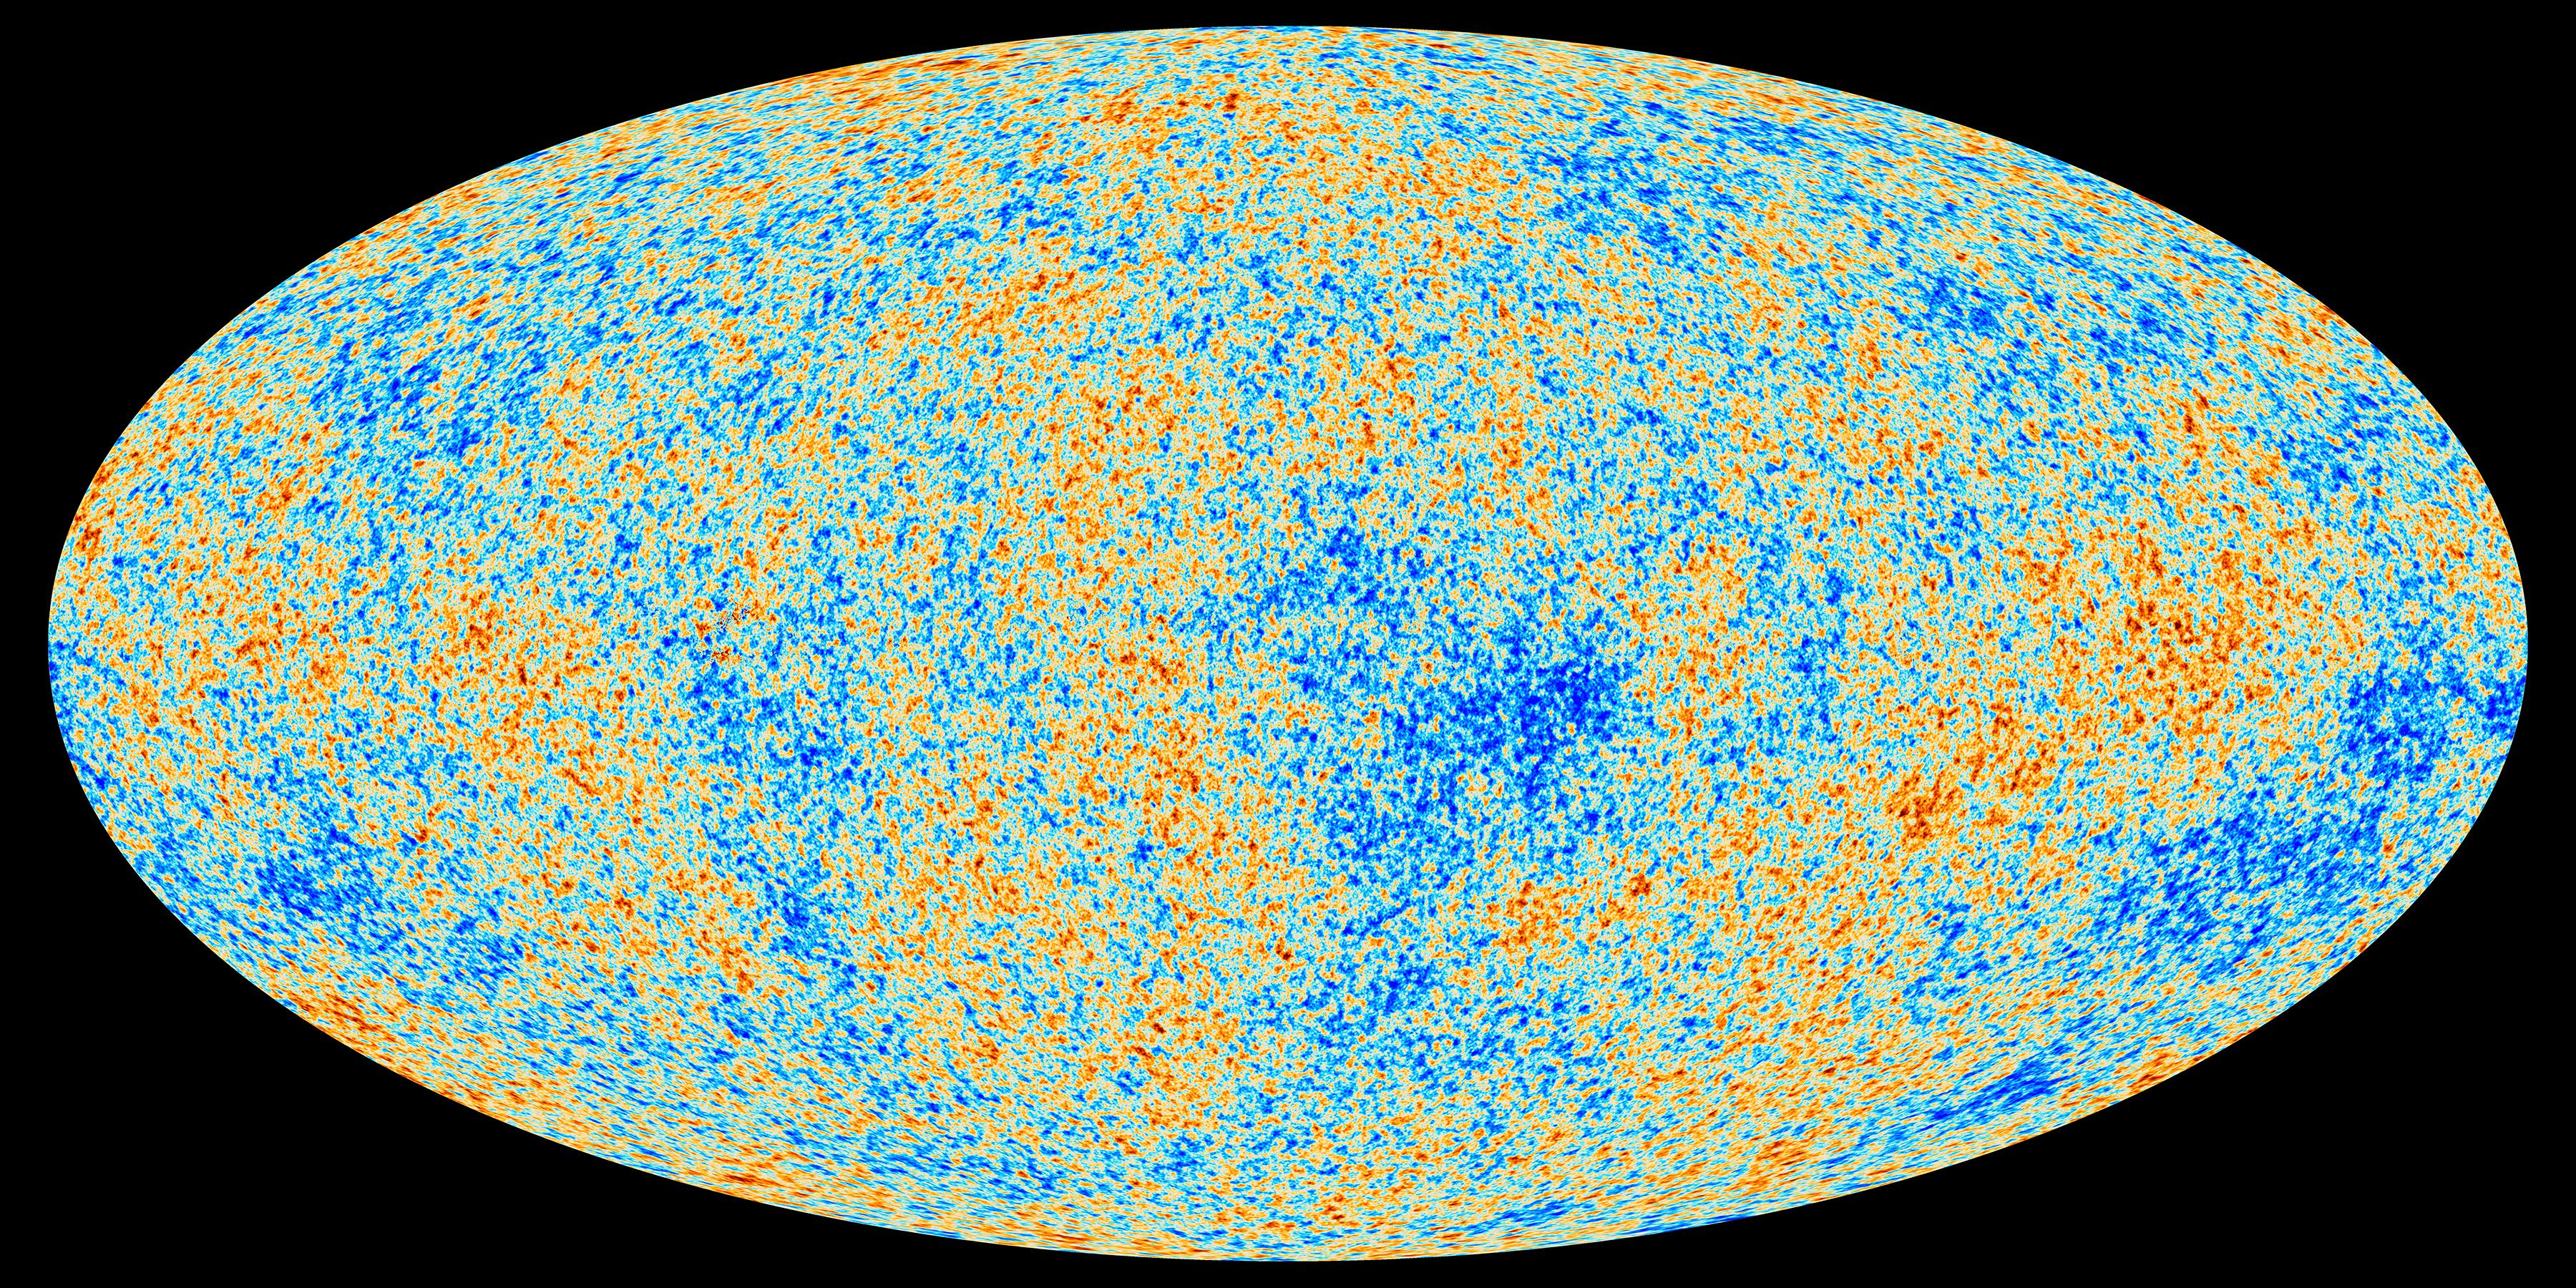
\includegraphics[width=0.9\linewidth]{figs/intro_figs/CMB_plank.png}
    \caption{Map showing the temperature fluctuations of the \gls{cmb} after all corrections are applied. The blue shows temperatures below the mean and the red shows temperatures above the mean. Image credit \cite{Planck:2013lks}}
    \label{fig:CMB_plank_2013}
\end{figure}

The Big Bang model predicts that relic radiation from the hot, dense early universe should still be observable today as a nearly uniform background. This prediction was confirmed in 1965, when Penzias and Wilson detected an unexpected, nearly isotropic background signal corresponding to a blackbody temperature of about 3.5\,$\degree K$ \cite{Wilson_CMB_obs}. More modern calculations have placed the average CMB temperature at 2.725\,$\degree K$ \cite{Fixsen_2009} with anisotropies at the level of $\pm 400\,\micro K$ \cite{Planck:2013lks}. These fluctuations, though small, provide one of our most powerful windows into the universe’s composition and early structure.

After applying necessary corrections to the \gls{cmb}, such as removing foreground emissions from the Milky Way, accounting for seasonal variations due to Earth’s orbital motion, and subtracting the Doppler, induced dipole anisotropy, we obtain the cleaned CMB map shown in Fig. \ref{fig:CMB_plank_2013}. Once these effects are removed, the remaining temperature fluctuations, though small, represent primordial anisotropies. These anisotropies provide detailed insight into the structure of the early universe and its physical composition. In particular, their characteristic scales encode the baryon–photon oscillations of the pre-recombination plasma.



The discovery of the \gls{cmb} provided an invaluable dataset, offering a glimpse into the early structure of the universe. Regions with higher matter density exhibited stronger oscillations, with the fundamental mode completing fewer than two full cycles before recombination. These oscillations imprinted themselves as peaks in the \gls{cmb} power spectrum, shown in Fig. \ref{fig:CMB_power_spectrum}. Each peak corresponds to a harmonic of the baryon–photon oscillations: odd peaks indicate compressions, while even peaks represent rarefactions. By analyzing the relative heights of these peaks, we can infer the amounts and types of matter and energy in the universe.



The peaks in this plot represent the strength (variance) of temperature fluctuations at different angular scales. Maximum variance occurs when the oscillations of the baryon–photon plasma are at either maximum compression (hotter regions) or maximum rarefaction (cooler regions). Odd-numbered peaks correspond to compressions, while even peaks correspond to rarefactions. The relative heights of the first and second peaks provide a measure of the baryon density: because baryons have inertia, the even peaks are suppressed compared to the odd ones. Dark matter, by contrast, does not couple to photons; it deepens gravitational potential wells without being affected by radiation pressure. In a universe with only baryons and photons, higher-order oscillations would be strongly damped, and the third peak would be suppressed relative to the second. Instead, observations show that the third peak is comparable in size, providing one of the clearest signatures of dark matter’s presence and abundance.

\end{comment}

\subsection{Cosmological Scale Evidence for Dark Matter}

\acrshort{dm} further helps explain the large-scale structure of the universe today. Without it, baryonic matter would not have had enough time to cool down via radiation to form the galaxies and galaxy clusters we see today. N-body simulations show that the distribution of galaxies and galaxy clusters we see today, including the cosmic web, could only be possible with \acrshort{dm} \cite{Benson_2010}. Under this theory, the small \acrshort{dm} halos that formed before recombination are expanded by inflation and some merge together over time. This leads to the formation of larger halos and more complex structures, leading to the universe we observe today \cite{cui2024knowhalomassfunction}. Further observations and calculations following the \gls{cmb} fluctuations to the present and analyzing the corresponding large-scale structure give further credibility to this claim \cite{sanchez_2011, PhysRevD.71.103515, Percival_2007}.


\subsection{Dark Matter Production}

To have the \acrshort{dm} we see in the universe, \acrshort{dm} must have a production mechanism, some way in which the high-energy early universe could produce \acrshort{dm}. Following Feynman's rules, if \acrshort{dm} has a creation mechanism, then it must also have an annihilation mechanism as Feynman diagrams are invertible \cite{PhysRev.76.769, Srednicki2007}. Under these conditions, over time \acrshort{dm} must have reached a thermal equilibrium in which it was being created and destroyed in equal amounts. As the universe expands and cools we can no longer generate new \acrshort{dm} particles. Later still in the evolution of the universe, \acrshort{dm} becomes sparse enough that annihilation interactions also do not happen. We refer to this process as ``freezeout" \cite{PhysRevLett.39.165}. After freezeout, the comoving number density for \acrshort{dm} is fixed and we calculate it as:

\begin{equation}
    \Omega_{\chi}h^2 = \frac{3 \times10^{-27}\frac{\text{cm}^3}{s}}{\langle\sigma v\rangle}.
    \label{dm_density}
\end{equation}

Now, for \acrfull{wimp}, dimensional analysis gives us $\langle\sigma v\rangle \approx \alpha^2/m^2_{\chi}$. If we plug in a value of 100\,GeV, which is in the weak scale, this gives us $\langle\sigma v\rangle = 3\times10^{-26}cm^3/s$ \cite{Steigman_2012}. Remarkably, when we now compute Eq. \ref{dm_density}, this gives a value of 0.1, which matches the observations with a value of 0.12. This is known as the \gls{wimp} miracle. 

This furthermore gives us a good insight into how to detect \acrshort{dm}. If we want to detect \acrshort{dm} via scattering with baryonic matter, we want to maximize the amount of energy imparted by the \acrshort{dm} particle onto our baryonic matter. For this we want full elastic scattering, so we want to use a target mass that is approximately 100\,GeV \cite{V_Chepel_2013}. Xenon happens to fit this bill with its most abundant isotope having a mass of $\approx 123$\,GeV.



\subsection{Current Knowledge of Dark Matter}

With the observational evidence for \gls{dm} established, the next step is to ask: what could it be? To guide this search, it is useful to first outline the key properties of \gls{dm}. From the evidence discussed in previous sections, we can infer the following properties of \acrshort{dm}:

\begin{itemize}
    \item \textbf{\acrshort{dm} is effectively electromagnetically neutral.} This comes from the \gls{cmb} power spectrum, since if \acrshort{dm} were strongly coupled to photons, this would be reflected in the fluctuations of the \gls{cmb} \cite{McDermott_2011}. 
    \item \textbf{\acrshort{dm} is effectively non-self interacting.} Observations of the Bullet Cluster show that if \acrshort{dm} were strongly self-interacting, its distribution would diverge from that of galaxies. Instead, it follows the galaxies, which behave like a collisionless gas \cite{Buote_2002, Harvey:2015hha}. 

    \item \textbf{\acrshort{dm} cannot be `hot'.} It does not move at relativistic speeds, since this would contradict the observed structure formation of the universe.
    
    \item \textbf{\acrshort{dm} has a minimum mass scale, depending on whether it is fermionic or bosonic.} The lower limits for fermionic \acrshort{dm} can be derived using Pauli's exclusion principle combined with the cosmological observations of galaxies and galaxy clusters, resulting in a lower limit of 70\,eV \cite{PhysRevLett.42.407, Randall:2016bqw}. In order to not conflict with the observations of the \gls{cmb}, bosonic \acrshort{dm} has a lower limit of $10^{-22}$\,eV \cite{Schive_2016, Nadler_2019}.
    
    \item \textbf{\acrshort{dm} is stable.} With a life-time comparable to or greater than the age of the universe, since it plays a key role in late-time structure formation. Estimates on the half-life of \gls{dm} have given it a lower value of 160\,Gyr \cite{Audren_2014}. In particular, the galaxy clusters we observe are not compatible with a large DM decay.
    
\end{itemize}

These constraints are stringent: combined, they exclude all known Standard Model particles. Any charged particle is ruled out, eliminating all quarks, charged leptons, and the W bosons. Neutrinos are fermions and have an upper bound mass estimate of 0.45\,eV \cite{KATRIN:2021uub}, much lower than the fermionic \gls{dm} 70\,eV limit. Gluons and photons are excluded because they are massless. Finally, the stability requirement rules out the Higgs and Z boson. %Not only this but due to the results of recent dark matter experiments, most of the fundamental forces have been ruled out of the WIMP paradigm as possible modes of interaction between WIMPs and baryonic matter \cite{Escudero:2016gzx}.

Alternative theories, such as modified gravity, have been proposed. However, none can simultaneously explain galaxy rotation curves, the Bullet Cluster, and the detailed features of the \gls{cmb}, which together probe \acrshort{dm} on galactic, cluster, and cosmological scales. These independent lines of evidence strongly favor a new particle component beyond the Standard Model. Among the many proposed candidates, one of the most theoretically well-motivated is the \gls{wimp}.



\subsection{Dark Matter Candidates}


\Glspl{wimp} are considered “massive” particles because their expected mass range lies between 20\,GeV and 100\,TeV \cite{Leane:2018kjk}, significantly heavier than most Standard Model particles. Direct detection experiments have already excluded large regions of the parameter space for \glspl{wimp} interacting via the weak nuclear force or the Higgs mechanism \cite{Escudero_2016}. Furthermore, from these experiments we have also ruled out \gls{dm}-nucleon cross section until regions close to the neutrino fog, the current \gls{dm}-nucleon cross section limits can be seen in Fig. \ref{fig:DM-nucleon_cs}. Nevertheless, this does not rule out \glspl{wimp} entirely; there remains the possibility that their interactions are mediated by a yet undiscovered fundamental force beyond the Standard Model.

\begin{figure}
    \centering
    \includegraphics[width=0.8\linewidth]{figs/intro_figs/DM-nucleon_cross_section.png}
    \caption{\acrshort{dm}-nucleon cross section as a function of \acrshort{dm} mass. Here we see the current limits from a variety of experiments. LZ has placed the most stringent limits for masses between 10 and 1,000\,GeV \cite{ref1, ref2, ref3, ref4, ref5, ref6, ref7, ref8, ref9, ref10, ref11, ref12, ref13, ref14, ref15, ref16, ref17}. Figure was generated using the \acrshort{dm} limit plotter made by Tarek Saab, University of Florida and Enectali Figueroa, Northwestern University.}
    \label{fig:DM-nucleon_cs}
\end{figure}

% Add cication ot the models
% Talk about pros and cons of each model

Several other \acrshort{dm} candidates have been proposed. Axions \cite{PhysRevLett.40.223, axion_paper}, for example, are a theoretical particle proposed as a solution to the unexpected absence of \acrfull{cp}-violation derived from quantum chromo-dynamics \cite{cp_problem_sym}. Axions are a good candidate for \acrshort{dm} due to their strong theoretical background; they could also be produced in the early universe just like \glspl{wimp}. Furthermore, their production mechanism makes them likely to be ``cold" today \cite{Sikivie_2008} and naturally give the correct abundance for \acrshort{dm} without fine-tuning \cite{DiLuzio:2020wdo}.

Primordial black holes are also a compelling candidate for \acrshort{dm}. Unlike black holes formed from dead stars, these black holes would be produced in overdense regions in the early universe \cite{blackhole_early_uni, PhysRevD.50.7173}. These black holes can span 40 orders of magnitude in mass ranges so there is a lot of flexibility in the possible masses \cite{PhysRevD.94.083504, bh_mass_constraint_1975}. Furthermore, black holes would not be affected by the radiation pressure in the early universe, matching the characteristics we know of \acrshort{dm} from CMB observations.

While these candidates are also very promising as \acrshort{dm}, we will not expand on them any further in this text. The XENONnT experiment is optimized to probe Weakly Interacting Massive Particles (\glspl{wimp}), making them the primary focus of this thesis. Here we will explain the xenon experiment, both in terms of hardware and software. Then, we will discuss unsupervised neural networks and how they are used to improve the signal classification in the XENONnT experiment. Finally, we will take a brief look at XAMS, a small \acrfull{tpc} experiment used to test the \gls{tpc} technology and see the impact of unsupervised classification on this data.


\newpage

\section{XENONnT Detector}

% Brief intro to the XENONnT detector

XENONnT's sophisticated detector design generates complex, multidimensional signals that demand equally
sophisticated classification methods. This chapter details the detector systems and physics processes that
produce the \acrfull{s1} and \acrfull{s2} signals, establishing the technical context for understanding why traditional
classification methods proved insufficient and motivating our development of \acrfull{som}-based approaches.

The XENONnT experiment is located at the \acrfull{lngs} in Italy, beneath the Gran Sasso mountain. This underground location provides shielding from cosmic rays~\cite{PDG2024CosmicRays}, atmospheric muons, and radioactive isotopes present at the surface, such as $^{85}$Kr, which is released during the reprocessing of spent nuclear fuel whose global atmospheric abundance is estimated to be 5,500 PBq at the end of 2009 \cite{AHLSWEDE201334}. This deep underground location reduces background radiation in the detector, simplifies background modeling, and improves sensitivity to rare events such as WIMP-nucleon scattering. The low-background environment at \gls{lngs} has already enabled the first observation of double electron capture in the previous-generation XENON1T experiment~\cite{doubleEcapture}.

XENONnT is the most recent and sensitive detector in the XENON series of liquid xenon-based experiments, designed to search for dark matter interactions with baryonic matter. The experimental setup consists of three nested subsystems: a dual-phase liquid xenon \gls{tpc} at its core, surrounded by a gadolinium-loaded water Cherenkov neutron veto, which is itself enclosed by an external water Cherenkov muon veto (Fig. \ref{xenonnt_diagram_all_detectors}). The primary science goal is the detection of \glspl{wimp}, which are hypothesized to elastically scatter off xenon nuclei in the \gls{tpc}, producing measurable scintillation and ionization signals~\cite{PhysRevLett.131.041003}. However, this is only one of several key science channels explored by XENONnT. Recently, the experiment reported the first observation of $^8$B solar neutrinos with a xenon target, in parallel with the PandaX-4T collaboration~\cite{XENON:2024ijk, PhysRevLett.133.191001}. This chapter provides an overview of the experimental apparatus, the underlying detector physics, and the data processing pipeline.

\begin{figure}[htbp]
    \centering
    \includegraphics[origin=c, width=16cm]{figs/xenonnt_bkg/Xenonnt_diagram_mod.png}
    \caption{Figure showing the nested detectors of the XENONnT experiment. The outer layer is the muon veto, the neutron veto sits inside with the cryostat and the \gls{tpc} at the core.}
    \label{xenonnt_diagram_all_detectors}
\end{figure}


\subsection*{Muon veto}

The muon veto is a cylindrical water tank measuring $\SI{9.6}{m}$ in diameter and $\SI{10.2}{m}$ in height, filled with approximately 700\,tonnes of demineralized water.
It contains 84 \acrfull{pmt}s, each 8\,inches in diameter, arranged into five vertically spaced rings along the tank's perimeter. When muons traverse the water, they emit Cherenkov radiation, which is detected by the \glspl{pmt}. These signals allow us to tag muons and veto events occurring in temporal coincidence with their passage~\cite{XENON:2024wpa}.
There are three primary reasons for vetoing data in the vicinity of a muon signal. First, muons can induce secondary interactions that mimic \gls{wimp}-like signatures, thereby increasing the background and reducing the ability to distinguish signal from noise. Second, vetoing muon-related data improves the signal-to-noise ratio by removing events associated with high-energy cascades, often accompanied by intense Cherenkov emission~\cite{JVJelley_1955}. Lastly, background models are constructed under the assumption that muon-induced events and their secondary interactions are excluded, improving the robustness and accuracy of background predictions.  

\subsection*{Neutron veto}

The neutron veto plays a direct role in reducing background events that can mimic dark matter interactions. It contains 33\,m$^3$ of water doped with gadolinium sulfate with 120 8-inch PMTs. When thermalized neutrons are captured, they emit $\gamma$-rays that Compton scatter electrons, accelerating them to relativistic speeds. These electrons then emit Cherenkov radiation, which is detected by the \glspl{pmt}. Gadolinium was added to enhance neutron detection efficiency, as it has the highest thermal neutron capture cross section among all stable elements. Upon capturing a neutron, gadolinium emits a cascade of $\gamma$-rays totaling 7.9–$\SI{8.5}{MeV}$, which produce Cherenkov radiation via Compton scattering~\cite{Wenz2023thesis}. The neutron veto is also useful in calibrating our detector for \acrfull{nr}. We use an AmBe source for neutron calibration, where, 
$$^{241}Am \rightarrow ^{237}Np + \alpha, ^9Be + \alpha \rightarrow ^{12}C^* \text{(or }^{12}C) + n$$

The de-excitation of $^{12}\text{C}$ produces a $\SI{4.4}{MeV}$ $\gamma$-ray~\cite{ITO2023168701}. When the  $\gamma$-ray is emmited, it interacts with the surrounding medium, which generates $\gamma$-rays detectable by the \glspl{pmt}. We use these $\gamma$-rays to tag these neutrons resulting from the excited carbon for our \gls{nr} calibration. The time coincidence between signals in the neutron veto and \gls{tpc} enables tagging of neutron-induced nuclear recoils. This significantly reduces background from neutron events, which closely mimic \gls{wimp}-like signatures.

At the core of the veto systems lies the dual-phase liquid xenon \gls{tpc}. This is the primary detector volume for dark matter searches and will serve as the central focus of this work.

\subsection{Dual-phase Liquid Xenon TPC}


The TPC contains a \acrfull{lxe} target with a small gas gap of \acrfull{gxe} forming a dual-phase configuration. Throughout this work, the term ‘TPC’ will refer specifically to this detector volume. The detector contains 5.9\,tonnes of \gls{lxe} within a cylindrical volume 1.34\,m in diameter. It is housed in a double-walled, vacuum-insulated cryostat that maintains the xenon at a temperature of $-98\,^\circ$C.
Light is detected by two arrays of 3-inch Hamamatsu R11410-21 PMTs: 241 PMTs at the bottom and 253 at the top, for a total of 494. This configuration maximizes \acrfull{lce} given the geometry of the \gls{tpc}. Maximizing the \gls{lce} is a crucial part of our experiment as it ensures accurate energy reconstruction of the interactions within the \gls{tpc}. To enhance photon collection, the \gls{tpc} walls are lined with \acrfull{ptfe} panels due to their high reflectivity for xenon scintillation light at $\SI{175}{nm}$~\cite{FUJII2015293}, with estimates as high as 97$\%$ in some studies~\cite{Neves:2016tcw}. The exact reflectivity in XENONnT, however, remains uncertain.

Electrodes are used to generate electric fields within the \gls{tpc}, which are necessary to extract electrons released during particle interactions in the liquid xenon. This enables us to measure the energy deposited into the ionization process. The electric field is shaped and maintained by five parallel grid electrodes and two concentric cages of field-shaping rings. The parallel grid electrodes are configured as follows (from bottom to top):
\begin{itemize}
    \item A screening mesh located $\SI{5.3}{mm}$ above the bottom PMT array.
    \item A cathode located $\SI{60}{mm}$ above the first screening mesh.
    \item A gate electrode $\SI{5.02}{mm}$ below the liquid level/$\SI{1.486}{m}$ above the cathode.
    \item The anode $\SI{8}{mm}$ above the gate.
    \item A second screening electrode $\SI{40.7}{mm}$ below the top PMT array.
\end{itemize}
To mitigate electrode sagging due to electric field stress and gravity, two perpendicular support wires were added to the gate and four to the anode. A uniform drift field of approximately $\SI{20}{V/cm}$ is established between the cathode and gate, directing ionization electrons upward toward the liquid-gas interface. There, an extraction field between 2.9–$\SI{3.7}{kV/cm}$, applied between the gate and anode, pulls electrons into the gas phase~\cite{XENON:2024wpa}. The field shaping electrodes maintain a uniform electric field within the TPC, which maximizes the active volume.

\Glspl{pmt} are the photon-sensitive components of the detector, responsible for converting scintillation light into measurable electrical signals. 
%Discribe how PMTs work -> data read out to DAQ -> data processing
When photons reach the photoemissive cathode, they produce \acrfull{pe}. The \glspl{pe} are accelerated toward a series of dynodes by an internal electric field. At each dynode, they release secondary electrons, resulting in signal amplification. The amplified electron cascade is collected at the anode, producing a voltage pulse proportional to the energy deposited in the interaction~\cite{hamamatsuPMT}. The analog signals are digitized at $\SI{10}{ns}$ intervals and passed to the \acrfull{daq}, where they undergo initial processing and are stored on dedicated servers.



\begin{figure}[htbp]
    \centering
    \includegraphics[origin=c, width=16cm]{figs/xenonnt_bkg/PMT-schematics.png}    \caption{Depiction of how PMTs work. We see that the emitted photons react with the photoemissive cathode to produce photoelectrons, which are amplified by the dynodes and read out by the anode. The change in voltage is correlated with the number of incident photons \cite{pmt_fig}. }
    \label{pmt_schematics}
\end{figure}


\subsection{Why Xenon?}

A natural question in the context of dark matter detection is: why choose xenon as the target medium? There are many reasons to choose xenon for our detector, which are the following:
\begin{itemize}
    \item \textbf{Noble Gas}: chemically inert, ensuring minimal interactions with detector materials and reducing unpredictable background sources. This helps maintain a low and well-characterized background rate. 
    \item \textbf{Maximizing WIMP Nucleon Cross-section}: The spin-independent WIMP-nucleon cross-section scales approximately with the square of the atomic mass number ($A^2$). Therefore, a heavy nucleus like xenon enhances the detection probability for WIMPs.
    \item \textbf{Stable atomic nucleus}: While heavier noble gases like radon exist, they are radioactive. Xenon offers a balance of high atomic mass and isotopic stability, making it ideal for low-background experiments.
    \item \textbf{Xenon is well-suited for scintillation-based detection}: Xenon has a high photon yield, and it is transparent to its own emissions, ensuring that the full energy of the interaction can be captured by the PMTs. This occurs because excited xenon atoms form short-lived dimers (excimers), which de-excite by emitting vacuum ultraviolet (VUV) photons. Since xenon is transparent to its own scintillation light, the emitted photons can travel significant distances without being reabsorbed.
    \item \textbf{Xenon is self-shielding}: Due to its high density, xenon is effective at attenuating external radiation. This self-shielding property enables background reduction by selecting a fiducial volume away from the detector boundaries.
    \item \textbf{Xenon has a low electron affinity}: due to its properties as a noble gas, making it easy for electrons to travel within the TPC and reducing the chances of the electron being absorbed.
\end{itemize}

There are other direct detection experiments that use different atoms such as argon, to conduct the dark matter search. Argon offers superior discrimination between nuclear and \acrfull{er} via \acrfull{psd}, which exploits differences in scintillation time profiles between the two interaction types. It is crucial to distinguish nuclear recoils from electronic recoils as \glspl{wimp} are expected to interact primarily via coherent scattering off atomic nuclei, whereas most background events produce \glspl{er} \cite{Lippincott2008}. 

However, most of the leading limits are set using xenon as a medium due to its higher atomic mass, which enhances the spin-independent \gls{wimp}–nucleon cross-section and improves sensitivity to \gls{wimp} signals. Additionally, for \glspl{wimp} with masses near $\SI{100}{GeV}$, xenon offers favorable kinematic matching, maximizing energy transfer during elastic scattering.

\subsection{From Light Signals to Data}

With the detector structure described, we now turn to the atomic interactions responsible for signal generation. When a particle interacts with a xenon atom in the \gls{tpc} it will impart some energy onto it. This energy deposition may occur via an \gls{nr} or an \gls{er}, depending on whether the particle interacts with the xenon nucleus or its electrons. The deposited energy results in two measurable channels: excitation, which produces scintillation light, and ionization, which frees electrons from xenon atoms~\cite{Lanqing2025thesis}. \Glspl{er} typically produce more ionization electrons, while nuclear recoils result in a higher proportion of scintillation light due to increased recombination and excitation. In this process, the recoiling xenon atom or electron will form a short track in which it will excite or ionize other xenon atoms, which form dimers with other xenon atoms \cite{VChepel_2013}. Through excitation, the process is simple:

$$Xe^* +  Xe +  Xe\rightarrow Xe_2^* +  Xe + heat$$

In the case of ionization, some freed electrons may recombine with xenon ions, forming excimers and contributing to the scintillation signal. This process is known as recombination~\cite{VChepel_2013}. Although the ionization pathway involves additional steps, it ultimately results in the same xenon excimer responsible for scintillation light:

$$Xe^+ + Xe \rightarrow Xe_2^+$$
$$Xe_2^+ + e^- \rightarrow Xe^{**} + Xe$$
$$Xe^{**} + Xe \rightarrow Xe_2^* + \text{heat}$$

Here, $Xe^*$ and $Xe^{**}$ denote two excited states of xenon with are two excited states of xenon, with $Xe^{**}$ representing a higher energy state. These xenon dimers will decay on the scale of 10~ns, releasing vacuum ultraviolet (VUV) photons with a wavelength of \SI{175}{nm}.

$$Xe_2^* \rightarrow Xe + Xe + \gamma$$

This mechanism underlies the primary scintillation (S1) signal observed in xenon detectors. Two distinct scintillation signals are produced in a dual-phase xenon TPC:
\begin{itemize}
    \item the prompt scintillation signal (S1), generated immediately at the interaction site, and
    \item the delayed electroluminescence signal (S2), produced when ionization electrons are extracted into the gas phase and accelerated, causing secondary photon emission.
\end{itemize}

Free electrons drift to the top of the \gls{tpc} due to an electric field, and are then extracted into the gaseous xenon with a stronger extraction field. These electrons excite xenon atoms in the gas phase, forming excimers that subsequently de-excite and emit vacuum ultraviolet (VUV) photons—this is the basis of the S2 scintillation signal. Scintillation light produced in the detector is recorded by \glspl{pmt} located on the top and bottom arrays (Fig. \ref{pmt_schematics}). 

\begin{figure}[htbp]
    \centering
    \includegraphics[origin=c, width=16cm]{figs/xenonnt_diagram.jpg}
    \caption{Diagram of the XENONnT TPC illustrating the production of S1s and S2s in our detector. On the left, we see an incoming particle interacting with the liquid xenon, producing scintillation light detected by the top and bottom PMT arrays, which produces a response that is faster in time than the S2. On the right, we see the released electrons from the initial interaction pass the liquid/gas interface, generating scintillation light that is detected primarily by the top PMT array, which is more localized. This signal also results in a signal that is more spread out in time due to the difference in arrival time of the released electrons. }
    \label{xenonnt_diagram}
\end{figure}

In addition to true S1 and S2 signals, several spurious or non-physical signal types can occur in the \gls{tpc} and must be identified and removed during analysis. Gas-phase interactions: particles can interact directly with the gaseous xenon above the liquid surface, producing a prompt signal that mimics an S1 and induces a weak S2-like response. PMT afterpulsing occurs when residual gas atoms inside the \gls{pmt} vacuum become ionized and later strike the photocathode, producing delayed signals.
Dark counts refer to spurious signals caused by thermionic emission or electronic noise in the \gls{pmt} circuitry. In what follows, we focus on the primary S1 and S2 signals that form the foundation of event reconstruction.

\subsection{Background and Calibration Data.}

While data taking, the types of runs in the XENON experiment can be largely classified into two types, background and calibration data. Background data is used to conduct most analysis like the \gls{wimp} and $^8$B search and it involves running the experiment while minimizing all outside radiation sources. During calibration runs, we deliberately introduce a known source of radiation into our experiment, either by injecting it directly into the liquid xenon and removing it later, or by putting a radiation source in a mechanism that can be placed next to the \gls{tpc}. 

\begin{figure}
    \centering
    \includegraphics[origin=c, width=10cm]{figs/ted_bkg_fit_xenon.png}
    \caption{Background event rates in the XENONnT experiment as a function of \acrfull{ces}. Figure shows the different components associated with the background in our experiment and how they all contribute to our overall background rate.}
    \label{xenonnt_background}
\end{figure}

\subsubsection{Background data}

XENONnT is an experiment that requires the lowest background radiation possible. Because of this, there was significant investment in the mitigation of potential outside sources of radiation \cite{XENON:2021mrg}. Despite all these efforts, it is impossible to make this kind of experiment free from all sources of radiation.
The background radiation detected in XENONnT is primarily for electronic recoils, produced by $\beta$-decay from $^{214}$Pb and $^{85}$Kr. 

\subsubsection*{Radon222}

$^{222}$Rn particles are almost unavoidable as it is ubiquitous on the Earth's crust \cite{epa_radon_origin}. As a result, $^{222}$Rn will be part of the material components used to build the detector, making it an unavoidable radiation source which we need to take into account in our background models. $^{214}$Pb is a byproduct of the decay chain of $^{222}$Rn \cite{PhysRevD.111.103040}, and with its half-life of just 26.8\,mins, it and its subsequent daughter particles are a substantial contributor to our \gls{er} background and our $\alpha$ background. As these contaminants cannot be completely removed, our aim is to model this background accurately and subtract it from our main science channel searches.

\subsubsection*{Kr85}

Xenon is sourced from the atmosphere which contains other gasses that are not easily separable. We expect other impurities will be present, such as $^{85}$Kr, a byproduct of nuclear fission, introduced into the atmosphere via nuclear testing and nuclear reprocessing plants \cite{bollhoefer2020}. $^{85}$Kr decays to $^{85}$Rb via beta decay, which means it is also a source \gls{er} background over a continuous energy range. While $^{85}$Kr is an intrinsic impurity, we can still reduce its concentration via a cryogenic distillation column \cite{Guida:2025lif}.

\subsubsection*{Xenon Isotopes}

Even if we obtained a perfectly pure sample of xenon, it still would not free us of intrinsic backgrounds as unstable isotopes of xenon are also present in the atmosphere namely: $^{136}$Xe and $^{124}$Xe. While undesired for the main \gls{wimp} search channels, these backgrounds also allow us to explore new physics. $^{136}$Xe produces 2 $\beta$ particles, this is known as double $\beta$ decay \cite{double_beta_decay, PhysRevLett.59.2020}. According to theory, this could produce a rare interaction known as a neutrinoless double $\beta$ decay, which, if found, would show neutrinos are Majorana particles \cite{PhysRev.56.1184}. This is one of our current science search channels \cite{PhysRevC.106.024328}. On the other hand $^{124}$Xe was already the subject of a significant observation by the XENON collaboration as in XENON1T, we observed the first documented case of a double electron capture \cite{doubleEcapture}. As such, these are backgrounds that we do not attempt to remove from our experiment and must be taken into account in our background models.

\begin{figure}
    \centering
    \includegraphics[origin=c, width=14cm]{figs/Rn_decay_chain.png}
    \caption{Decay chains for Rn 222, a common source of background radiation in XENONnT and Radon 220 which is used as a calibration source. Figure credit \cite{Rn222_decay_chain}}
    \label{rn_decay}
\end{figure}

\subsubsection*{Neutrinos}

This is for all neutrinos, not just solar.
The sun produces neutrinos, which contribute to the background of our experiment; these are called solar neutrinos. These neutrinos can contribute to our background both via ER scattering and scattering off the nucleus of xenon atoms known as \acrfull{ceνns}. The signal produced by a CEνNS interaction is almost identical to a 6\,GeV/$c^2$ WIMP \cite{PhysRevLett.126.091301}. ER of neutrinos can be excluded from our analysis with relative ease however, NR recoils of neutrons is a major limitation of the WIMP search analysis.

\subsubsection*{Accidental Coincidences}

\acrfull{ac} are an artifact of our event reconstruction as they occur when we incorrectly pair an S1 and S2 signals. ACs can occur for a number of different reasons, including the misclassification of a single electron S2 signal as an S1. We refer to these S1/S2 signals that could be mismatched as ``isolated", as they lack a corresponding S2/S1 signal to match with. ACs happen when these signals occur within the event building time window \cite{PhysRevD.100.052014}. We calculate the background rate of ACs with a data-driven analysis and the formula: 
$$R_{AC} = R_{isoS1} \text{ x }R_{isoS2} \text{ x } \Delta t.$$

Where $R_{isoS1/S2}$ is the isolated S1/S2 rate and $\Delta t$ corresponds to the event building time window. To minimize the number of ACs in our analysis, we developed a gradient boosted decision tree classifier based on the S2 pulse shape and drift time to flag and exclude these signals \cite{PhysRevD.111.103040}.

\subsubsection*{Material Background}

% We dont we have to worry about the daughter products of Rn222 until lead
The XENON Collaboration built the XENONnT experiment using material screened for radiation to minimize background radiation from materials; however, obtaining materials with no radioactive impurities is almost impossible and extremely expensive. The \gls{tpc} walls are made of \gls{ptfe}, has been documented to absorb $^{222}$Rn \cite{Rn222_decay_chain}. This isotope of Rn is highly unstable and quickly decays to $^{210}$Pb. Following this decay chain we can expect two $\beta$ decays from $^{210}$Pb and $^{210}$Bi followed by the $\alpha$-decay of $^{210}$Po. Since we know the source of these events comes from the walls, we can heavily reduce this background by applying a fiducial volume cut whose boundaries we can determine by examining the monoenergetic $\alpha$ events from $^{210}$Po \cite{PhysRevD.111.103040}.

\subsubsection{Calibration data}

XENONnT has numerous radioactive isotopes it uses for detector calibration. In particular, calibration sources such as $^{83m}$Kr, $^{241}$AmBe, $^{220}$Rn and $^{37}$Ar are used to quantify the detector response to ionization radiation \cite{xenoncollaboration2024xenonntanalysissignalreconstruction}.  While we will not discuss all calibration sources here, we will go through the calibration sources relevant for this article.

\subsubsection*{Rn220}

$^{220}$Rn is used to calibrate the detectors' \gls{er} response. The decay chain of this atom provides a continuous \gls{er} spectrum at low energies thanks to its $\beta$ emitter daughter and is used to model our \gls{er} band \cite{Lang:2016zde, xenoncollaboration2024xenonntanalysissignalreconstruction}. Due to its shorter half-life of 55.8\,seconds, this isotope of Rn can be used for calibration as it quickly decays into $^{208}$Pb, which is not radioactive \cite{Murra:2022mlr}, making it safe to resume normal background runs shortly after.

\subsubsection*{Kr83m}

$^{83m}$Kr is a metastable version of Kr which decays producing 2 $\gamma$-rays of 32.1 and 9.4\,KeV with decay half-life of 1.83~hrs and 154~ns respectively \cite{Kastens:2009pa}. As with radon, $^{83m}$Kr can be injected directly into our detector and its slow first half-life gives enough time for a uniform distribution, making it useful for calibration of detector response as a function of spatial location. Furthermore, the mono-energetic decays can also be used as a sanity check to measure our ability to reconstruct the energies of these interactions.

\begin{figure}[htbp]
    \centering
    \includegraphics[origin=c, width=6cm]{figs/kr_decay_energies.pdf}
    \includegraphics[origin=c, width=9cm]{figs/kr83_decay.pdf}
    \caption{$^{83m}$Kr decay. Left: $^{83m}$Kr decay before becoming stable. Right: possible peaks we expect for the $^{83m}$Kr decay; bottom two plots show complications in the data, such as the merging of peaks that are close together in time. Figure credit: \cite{kr83_dacay}}
        \label{Kr_decay}
\end{figure}

\subsubsection*{AmBe}

$^{241}$AmBe is our neutron calibration source, which releases a neutron when Am decays and produces an $\alpha$ particle that is absorbed by the Be, which becomes carbon and emits a neutron. For a detailed description of this process, see \cite{Wenz2023thesis}. This calibration source produces neutrons in a continuous energy spectrum and, as such, can be used to model our \gls{nr} band. The source for this neutron emitter is located outside the \gls{tpc} cryostat, which means we can use the neutron veto to tag some of these events.

\subsubsection*{Ar37}

We use $^{37}$Ar for the calibration of low-energy interactions of \gls{dm}. $^{37}$Ar decays via electron capture and, depending on the electron shell the captured electron came from, produces different signals. If $^{37}$Ar captures an electron from the K-shell, it emits a 2.8224\,keV S1 signal and a corresponding ionization signal. If $^{37}$Ar captures an electron from the L-shell, it only produces an S1 signal of 0.2702\,keV. The photons released from this interaction are not energetic enough to ionize Xe; therefore, they do not produce S2 signals \cite{Boulton:2017hub}.

\subsection{Software Infrastructure}

To manage the complex chain of data processing, metadata tracking, and security, the XENON collaboration has developed a number of different packages to aid in our work. At the core of the data processing are \hyperlink{https://github.com/AxFoundation/strax}{Strax}, \hyperlink{https://github.com/XENONnT/straxen}{Straxen}, and \hyperlink{https://github.com/XENONnT/cutax}{Cutax}—-packages that handle waveform processing, XENON-specific extensions, and cut definitions, respectively. These packages operate through a plugin architecture, where each plugin is a class responsible for a specific step in the data processing chain. A configuration object called a context defines which plugins to use and manages the necessary metadata for each analysis which is handled by \hyperlink{https://github.com/XENONnT/xedocs}{Xedocs}. \hyperlink{https://github.com/XENONnT/utilix}{Utilix} is used for general configuration and provides access to the runs database, which stores metadata about processed data runs. A run refers to a continuous period of data acquisition, typically characterized by its duration and data type (e.g., calibration, background, science), and is referenced by its unique run\_ids. We will discuss the software infrastructure in more detail in Sec. \ref{sec: Software_Infrastructure}.


\begin{comment}
data processing and other day to day organizational infrastructure the XENON collaboration has developed a number of different softwares with different applications. 
\begin{itemize}
    \item \hyperlink{https://github.com/AxFoundation/strax}{Strax}: an analysis framework for pulse-only digitization data. It is mainly build to support noble liquid TPC experiments such as XENONnT.
    \item \hyperlink{https://github.com/XENONnT/utilix}{Utilix}: utility package serving 2 main functions: (1) a general xenon configuration framework and (2) grants access to our runs database.
    \item \hyperlink{https://github.com/XENONnT/xedocs}{Xedocs}: Used for reading and writing to our metadata dataabse, which include corrections used for data processing.
    \item \hyperlink{https://github.com/XENONnT/straxen}{Straxen}: Main software for data analysis of the XENONnT collaboration, built on top of strax and integrates utilix and xedocs. Converts data from raw PMT readouts to energy meassurments of the intractions.
    \item \hyperlink{https://github.com/XENONnT/cutax}{Cutax} Software build on straxen, used to manage cuts for data cleaning necessary for data analysis.
\end{itemize}
We will expand on the software infrastructure in a later chapter.
\end{comment}

\subsection{Data corrections}

To accurately reconstruct particle interactions in the detector, we apply corrections at multiple stages throughout the data processing pipeline. These include corrections for converting PMT voltage traces to photoelectrons (during record formation) and accounting for the electron drift velocity to reconstruct the interaction depth. We use xedocs to manage the metadata associated with each correction, while enforcing rules and constraints to preserve data integrity during schema updates.
Some of these corrections or schemas, as we will call them henceforth, need different rules.


One key correction is the electron lifetime correction. As electrons drift through the liquid xenon, some are absorbed by electronegative impurities, reducing the number that reach the gas phase and contribute to the S2 signal. The electron lifetime characterizes this absorption and is used to correct the S2 area by extrapolating it to what would have been observed with infinite purity. Since electron lifetime changes over time, it must be carefully tracked and applied per-run. This is one of many time- and position-dependent corrections, making robust metadata handling essential—precisely the role of xedocs.

The metadata corrections tend to vary the most between different \acrfull{sr}. Science runs are designated time periods in which we collect data with the aim of publishing a result, usually to release our WIMP analysis. As of writing, XENONnT has had 3 science runs: SR0, SR1, and SR2. SR0 occurred shortly after the end of the commissioning phase of our detector and was used for our first set of results. After we were done with the analysis for SR0, we decided to make significant changes to the configuration of the detector for SR1. Major changes in the detector usually occur between science runs. For our purposes, we will only focus on the changes between science runs that affect low-level data. Between SR0 and SR1, there were significant changes to the way we adjust the PMT gains, affecting the characteristics of the waveforms generated. For our purposes, there is no difference between SR1 and SR2.


\subsection{Achievements of the XENONnT Experiment}

\subsubsection{WIMP constrain}

In February 2025, XENONnT released its latest results from the search for WIMP elastic scattering on xenon nuclei, combining the results of their two science runs (SR0 + SR1). The datasets consisted of 186.5 (95.1)\,days of livetime in SR1 (SR0) for a total exposure of $\SI{3.1}{tonne\cdot year}$. No significant excess above background was observed for nuclear recoil energies above $\SI{3.8}{keV_{nr}}$. We set a new upper limit in the spin-independent WIMP-nucleon scattering cross section for WIMPs of masses above 10\,GeV/c$^2$. The lowest cross-section limit reached was $1.7 \times 10^{-47}$\,cm$^2$ at 90\% confidence level for a WIMP mass of 30\,GeV/c$^2$. The best median sensitivity achieved was $1.4 \times 10^{-47}$\,cm$^2$ for a 41\,GeV/c$^2$ WIMP \cite{XENON:2025vwd}. Although we did not achieve a lower limit than LZ with our current data, the validation of the dark matter exclusion cross section is still an important check (Fig. \ref{wimp_results}).

\begin{figure}[htbp]
    \centering
    \includegraphics[origin=c, width=12cm]{figs/xenonnt_bkg/wimp_nucleon_cross_section_2024.png}    \caption{WIMP-nucleon cross section limits as a function of WIMP mass for the leading direct detection dark matter experiments. We see that while we obtained a lower limit than PandaX-4t the leading sensitivity, are places by LZ in this channel \cite{XENON:2025vwd}.}
    \label{wimp_results}
\end{figure}

\subsubsection{Detection of Solar neutrinos}

In November 2024, the XENON collaboration published a paper detailing the first measurement of nuclear recoils from $^8$B solar neutrinos via CEνNS. We conducted a blind analysis with an exposure of {3.51}\,{tonne$\cdot$yr} resulting in 37 observed events above 0.5\,keV compared to a background expectation of $26.4^{+1.4}_{-1.3}$ events. This corresponds to a rejection of the background-only hypothesis with a significance of 2.73$\sigma$ \cite{XENON:2024ijk}. The measured $^8B$ solar neutrino flux is consistent with the observations at the Sudbury Neutrino Observatory \cite{SNO:2011hxd}. We also report that the measured neutrino cross section on Xe is consistent with the Standard Model predictions. This marks the first direct detection of nuclear recoils from solar neutrinos using a dark matter detector \cite{XENON:2024ijk}.

\begin{figure}[htbp]
    \centering
    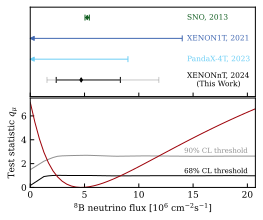
\includegraphics[origin=c, width=12cm]{figs/xenonnt_bkg/b8_unblinding_1d_cl_68.png}    \caption{$^8B$ neutrino flux for different experiments. We see that the tighter limits were set by SNO in 2013 \cite{SNO:2011hxd} with a dedicated neutrino experiment. In the latest XENONnT results, we obtained a tighter constraint from other direct detection dark matter experiments, results which are consistent with SNO.}
    \label{b8_results}
\end{figure}

\subsection{Scope}

In this document, we primarily focus on two dark matter detectors. These are the XENONnT detector, designed to detect dark matter and other rare interactions, and the XAMS experiment, which aims to test emerging TPC technologies.

Both experiments operate under the same physical principles and share a similar software architecture for data analysis. The differences between the two will be discussed when needed but we focus primarily on XENONnT, as the Nikhef-based XAMS detector serves as a simplified test platform for its technologies. This section emphasizes XENONnT, with a more detailed discussion of XAMS provided in later chapters.

\newpage

\section{Software Infrastructure in the XENONnT Experiment}
\label{sec: Software_Infrastructure}

The processing of XENONnT's petabyte-scale data requires sophisticated software infrastructure that enables both standard analyses and novel classification methods. This chapter describes the computational framework that made our \acrfull{som} implementation possible, detailing how we integrated machine learning approaches into the existing pipeline while maintaining the collaboration's requirements for reproducibility and performance.

The XENONnT experiment collected $\approx1.9$\,PB of data in the first two years of operation, bringing us to an average of almost 1\,PB per year \cite{tda_Aprile_2023}, making large-scale software infrastructure a necessity for our experiment. Furthermore, robust software infrastructure reduces the computational overhead associated with debugging and resolving software issues, maximizing the time analysts spend on physics analysis. Adequate software infrastructure also plays a critical role in ensuring reproducibility, an essential part of scientific research.

\subsection{Introduction}

%\subsubsection{Motivation}

Modern high-energy physics experiments rely on complex and large-scale software infrastructures to manage their increasing data volume and analytical complexity. This is particularly important in medium to large-scale experiments, which require sophisticated tools and scalable infrastructure to process complex scientific data \cite{jacobs2025whitepapersoftwareinfrastructure, Clemencic_2017, HEPSoftwareFoundation:2017ggl, agapopoulou:hal-05018428}. 


%\subsubsection{Data complexity}

The data categories are largely separated into low-level, peak-level, and event-level data. Each of these types of data requires sophisticated processing techniques to address the goals and challenges at each step. After collecting low-level \gls{pmt} signals, we need to combine them into peaks. Individual \gls{pmt} signals need to be integrated in time to form peaks. Ideally, each peak would correspond to one physical interaction, but ensuring this often requires more data processing. This is done by applying recursive peak splitting algorithms and recombining some signals when necessary. From each peak, we extract properties such as area, width, and timing, which are used in event building and energy reconstruction. These corrections are dependent on time-varying detector conditions which can change gradually or abruptly due to calibration runs and environmental or operational changes that impact detector response. 

%\subsubsection{software solutions}

To face these challenges, the XENON collaboration has built its own set of software packages to address issues like data processing and condition data management, and uses existing software such as Rucio to handle data transfers.

The core of the XENONnT software infrastructure consists of Strax, Straxen, and several supporting packages such as Cutax and xedocs. These software packages were built with heavy consideration towards collaborative software development. Strax(en) has extensive documentation that can be found here \cite{strax_main, straxen_pipeline}. These software are highly modular, plugin-based pipelines designed for quick and reliable data processing and ease of interoperability for future developers. Reproducibility is a fundamental requirement in any scientific experiment, but it is particularly challenging in large, evolving software environments like XENONnT. For that, we developed a system of lineage hashes to ensure that data sets processed with different configurations would not be confused with each other.


Changes to the data processing pipeline are implemented by creating new Python classes or plugins to compute specific features, corrections, or physics quantities. To ensure the integrity of our codebases, we require all code changes must be reviewed and approved by at least one other analyst via GitHub pull requests. We make our software stack maintainable through documentation and encourage the reuse of code, two of the most important qualities for scientific software development \cite{ARVANITOU2021110848}. Major changes to the code are also discussed in a dedicated group meeting for those working in the computing infrastructure in XENONnT, known as Team A. We also encourage members of different groups within the XENON collaboration to take on some computing tasks to try to lift the burden of those working in computing.

In the following sections, we first introduce the XENONnT data flow pipelines. We then describe the core software tools, data processing schemes, and metadata management strategies. Finally, we discuss our data storage infrastructure and propose improvements for future scalability.

\subsection{Data flow pipeline}

%\subsubsection{DAQ and Raw Data Collection at LNGS}


To manage the distribution and cataloging of raw data beyond \gls{lngs}, we rely on the Rucio, a data management system originally developed for ATLAS but now adopted in many major particle physics experiments \cite{Barisits_2019}. We primarily interact with Rucio through a XENON-specific interface called Admix. 

Admix is a Python middleware that provides experiment-specific abstractions, including automated MongoDB synchronization, safety-enhanced data operations and specialized template systems for data organization. Admix also provides some important advantages such as two-fold data verification before operations, automatic backup validation and it seamlessly integrates with XENON's existing MongoDB run database. Admix initiates the data distribution to further worldwide distributed \acrfull{rse}s for data storage. Once the data have been uploaded to the buffer disk for Rucio distribution, a copy is also archived to tape storage, which is isolated from the distributed RSEs. The meta-database of runs is updated with the RSE information by Admix when a data transfer is fulfilled \cite{Ahlin_2019}.


Most of our data processing is done via the \acrfull{osg}, which provides the distributed computing foundation for XENONnT's computational needs. This infrastructure delivers over 1.2 billion CPU-hours annually across 100+ sites, with HTCondor-CE serving as the primary job gateway \cite{osg_htc}. 

We interact with OSG via the \acrfull{rcc} at the University of Chicago, which provides high-performance computing via Dali, midway2 and midway3. Dali will be decommissioned in the near future; however, we currently use it to store peak-level data. Midway2 on the other hand delivers 16,016 cores across 572 nodes \cite{uchicago_rcc_hpc} while Midway3 offers over 10,100 cores plus GPU resources and accelerators \cite{uchicago_midway3}.

The raw data from our \glspl{pmt} is processed by our \acrfull{daq}. 
Our DAQ is a triggerless system that reads out the \glspl{pmt} from all 3 detector subsystems and, thanks to custom-developed software, live data is available within $\mathcal{O}$(10s) of the readout 
and stored on a 50\,TB disk at \gls{lngs} \cite{tda_Aprile_2023}. The data the flows from \gls{lngs} through the Strax processing pipeline, with Admix managing automatic upload to our distributed storage and enforcing rule-based replication. A copy of the data is written to a second buffer disk, which serves as a Rucio Storage Element (RSE).
This allows for continuous data taking in case of a network issue, preventing the data from being transferred to the external storage. This pipeline and data distribution enables all our collaboration members to access the data efficiently while maintaining strict data integrity standards.

%\subsubsection{Low-Level Processing on OSG and intermediate data handling}

Low-level processing begins once raw data are registered in the Rucio catalogue and available at a recognized RSE. These raw files, which contain digitized \gls{pmt} waveforms from all detector subsystems, are the primary inputs to the first processing stage. These data are processed using the OSG, running computationally intensive algorithms to identify and classify peaks, compute low-level features, and apply initial calibrations. The resulting intermediate data products are collected at the dCache storage facility in Chicago, then transferred to the Research Computing Center (RCC) at chicago via Admix using the underlying scp transfer mechanism. Because these intermediate files are rarely used directly by analysts and serve primarily as a bridge to high-level data products, only the latest versions are stored in Dali and tracked through the Rucio catalogue. The metadata database is updated accordingly with the new file locations \cite{Ahlin_2019}. 

High-level data processing builds on the outputs of low-level processing to generate events and compute derived quantities that depend on those events. These data are moved to analysis-specific directories within the RCC storage system, where they are directly accessible to analysts \cite{Ahlin_2019} via the Midway2 and Midway3 machines. Admix is used to manage uploads and downloads between all of our data storage sites, facilitating data movement between distributed storage locations and the local cluster. This stage marks the final step in the data pipeline, producing analysis-ready datasets that serve as the foundation for physics results.

% Need to work on the order of things in this section.

\begin{figure}
    \centering
    \includegraphics[width=0.9\linewidth]{figs/software/xenon_data_stream.png}
    \caption{Data flow from production at \gls{lngs} to the metadata storage and data storage, including high level processing with OSG. Data from the DAQ is sent to Disk at \gls{lngs} for temporary storage where the rucio servers aid us in their distribution. The metadata produced along with this files is stored at the RunDB, all other data is distributed amonst storage sites contributed by different institutions collaborating in our experiment. For the UChicago machines we initiate the data processing and the resulting data is stored at UChicago in the Dali and Midway machines. A copy of all of our raw data is stored in tape at CNAF for long term storage.}
    \label{fig:xenonnt_dataflow}
\end{figure}

\subsection{Core Software Components}

One fundamental difference that makes the XENON software stack stand out is that it is one of the first to be written in Python for a large physics collaboration or experiment. Traditionally, languages like C, C++, and FORTRAN are used for their optimized speed in comparison to higher-level languages. While Python is not traditionally known for speed, optimized libraries and modern techniques have narrowed the performance gap with compiled languages. We describe these optimizations in detail in Section~\ref{sec:optimization}. Using Python also helps address a major challenge in scientific software development: managing and maintaining large, evolving codebases. Python’s user-friendly syntax and high-level abstractions make it easier to learn and use than most traditional languages \cite{ARVANITOU2021110848}.

Our main software infrastructure focuses on the Python packages Strax, Straxen, and Cutax. Straxen extends Strax with experiment-specific functionality for XENONnT, while Cutax builds on Straxen to implement common data selections. These packages expose a plugin-based framework that allows users to flexibly define and run data processing pipelines. From the user side, they primarily work by establishing a \textit{context}, which registers the storage for both data and metadata, registers plugins, and connects it to processors (Fig. \ref{strax_context}). The context abstraction enables modular and reproducible workflows by encapsulating all relevant inputs and settings for a given processing task. A \textit{context} also has all the information needed to establish the lineage of a particular data type, which ensures we do not mix up data processed with different plugin configurations or code versions.

\begin{figure}[htbp]
    \centering
    \includegraphics[width=0.9\linewidth]{figs/software/strax_context.png}
    \caption{In our core software infrastructure a user defined a contexts which registers the storage and plugins that will be used for processing. When data is generated using the context the processor utilizes the plugins for processing and uses the loader to access data from out corrections database needed to generate the desired outputs. A saver function then stores the data in disk for the user to access, image credit \cite{aalbers2018strax}.}
    \label{strax_context}
\end{figure}


\subsubsection{Strax}

\begin{comment}
    
\begin{itemize}
    \item Streaming analysis framework. Efficiency and scalability
    \item Plugin-based design for data processing.
    \item Data types: records, peaklets, peaks and events. Also talk about data types vs data kinds.
    \item Talk about context and storage.
\end{itemize}

\end{comment}

Strax is an analysis framework designed for processing pulse-only digitized \gls{pmt} data, specialized for live data processing at speeds of 50-100\,MB(raw)/core/sec \cite{strax_main}. As the experiment expanded and the rate of data increased, the previous processor pax \cite{pax_xenon1t} became insufficient to meet these needs. As a result, Strax was developed as a general framework for this kind of analysis. To achieve the required performance improvements, Strax leverages NumPy structured arrays and Numba for just-in-time (JIT) compilation, which together achieve a performance improvement of 100x compared to interpreted Python \cite{strax_main}. 

\subsection*{Performance optimizations (numpy/numba)}
\label{sec:optimization}

NumPy is a Python package for scientific computing. It enables vectorized operations, which replace explicit Python loops with efficient array-level computations implemented in optimized C code. This enables quick and efficient array computations and matrix operations. NumPy supports multidimensional arrays and derived objects such as masked arrays, which allow for conditional computations and other routines for quick operations on these objects. Furthermore, NumPy arrays are stored in contiguous blocks of memory, which allows for efficient indexing and better CPU cache performance \cite{numpy_docs}. In practice, this means we can perform operations over waveforms, which are 200-element arrays, and compute derived quantities for a set of interactions with better efficiency than using loops. Given the scale of data processed in XENONnT, optimizing performance with NumPy is essential to keep analysis pipelines efficient and scalable.
% Might need more details on numpy

While NumPy optimizes array operations, Numba addresses Python's computational limitations through just-in-time compilation. This complementary approach enables a number of optimizations for Python code that make compatible functions compute at speeds comparable to compiled languages such as C/C++, examples of this can be seen in \cite{murillo_numba_vs_c, fua2020comparingpythongoc}. Numba achieves this due to its following properties:

\begin{itemize}
    \item Just-in-time (JIT) compilation. Unlike static compilation, where a program is compiled before execution, JIT compilation compiles code at runtime, just before it is executed \cite{history_of_jit}, leading to significant speed boosts of the program.
    \item Numba uses Low-level virtual machine (LLVM) as an intermediate representation of the code on which optimizations can be performed before things are translated to machine code \cite{murillo_numba_vs_c}.
    \item Bypassing Python type checking. The features that make Python easy to use—such as dynamic typing—also contribute to its slower execution. In Python, we do not have to declare the data types. This makes Python very flexible, but it also makes it so we do not have code optimized to a particular data type. Additionally, Python code has to constantly check data types to ensure operations are valid. With numba, we declare and specify a data type, which enables us to bypass checks and use more optimized code when translating it to machine language for execution.
    \item Bypassing the Python Global-Interpreter-Lock (GIL), which makes it so that only one computer core can handle operations. This is done as a safety precaution and so that users do not need to deal with memory locations, unlike other languages. By releasing the GIL, we can access multithreading, enabling parallel execution of loops across multiple threads.
\end{itemize}

In Strax, we use Numba to accelerate computationally intensive tasks such as baseline computation in raw\_records and efficient chunking of waveform data for storage. These optimizations are critical for maintaining real-time processing capabilities given the volume of data produced by XENONnT.

\subsection*{Parallelism and memory layout}

Memory access latency and bandwidth limitations are often major bottlenecks in data-heavy pipelines \cite{memory_wall1995}; as such, this aspect was also addressed when transitioning from PAX to Strax. In Strax, we transitioned from object-oriented data structures (such as dictionaries and custom classes) to an array-oriented programming model. This allows us to saturate the memory bus to the CPU cache, drastically reducing the time spent in moving memory, thus making data analysis much quicker. Using structured arrays enables faster data access and caching, typically one of the slowest aspects of high-energy physics analysis \cite{Pivarski_2018}. By taking advantage of numpy structured arrays, the data does not need to be constantly copied, and instead we can use views and references. This minimizes memory movement, and takes advantage of SIMD vectorization, and allows the CPU caches and prefetchers to be fully utilized, leading to saturation of the memory bandwidth.  Furthermore, having objects for each interaction presents a problem for data analysis, as fetching data from objects requires nested functions/protocols. We can see an example of the difference in computation speed by looking at the computation rate for CMSSW [tab \ref{tab:HEP_query_systems}] where we can see that analyzing the full framework of an event is 6 orders of magnitude slower than direct operation on arrays. This can be likened to optimizing a shuttle service: maximizing the number of passengers per trip and avoiding redundant back-and-forth trips reduces overall travel time. 

To quantify these improvements, PAX achieved processing speeds of $\mathcal{O} (\SI{100}{kB/s/core})$, while Strax can process data at rates of $\mathcal{O} (\SI{100}{MB/s/core})$ \cite{tda_Aprile_2023}.

\begin{table}[]
    \centering
    \begin{tabular}{c|c}
         0.018 MHz & full framework (CMSSW, single-threaded C++) \\
         0.029 MHz & load all 95 jet branches in ROOT \\ 
         2.8 MHz & load jet pT branch (and no others) in ROOT \\ 
         12 MHz & allocate C++ objects on heap, fill, delete \\ 
         31 MHz &  allocate C++ objects on stack, fill histogram \\ 
         250 MHz &  minimal “for” loop in memory (single-threaded C) \\ 
    \end{tabular}
    \caption{Rate of processing a payload of filling one histogram of jet pT for all jets in a tt¯ sample at CMSSW. Table illustrates the orders of magnitude of time lost to providing a full framework for heavy event processing, all single-threaded \cite{Pivarski_2018}.}
    \label{tab:HEP_query_systems}
\end{table}

\begin{comment}
\begin{figure}[htbp]
    \centering
    \includegraphics[origin=c, width=14cm]{figs/software/speed_comparison_numba_c.png}
    \caption{Comparing computing speeds for python, python + numba and C++ applied to simple cellular automata (CA) models. This is meant as an example to illustrate general trends seen in the literature and not as an exhaustive figure. Img credit [https://murillogroupmsu.com/numba-versus-c/]}
    \label{numba_speed}
\end{figure}
\end{comment}

\subsubsection*{Plugin based design}

One of the key architectural choices behind Strax is its plugin-based design, which contributes significantly to its scalability. This decision was motivated in part by historical factors: many collaborators in the XENON experiment were already familiar with this modular structure. Moreover, the plugin model aligns well with the collaborative nature of the experiment, enabling individual developers to work independently on specific components without requiring extensive coordination. This mirrors Conway’s Law, which states: “Any organization that designs a system will produce a design whose structure is a copy of the organization’s communication structure” \cite{conway_committees, conway_law}. In XENON, communication often takes place within smaller subgroups, each responsible for a particular aspect of detector performance or analysis. The plugin architecture reflects this organizational structure by allowing distinct contributions to be integrated smoothly into the larger data processing pipeline.

Technically, each plugin in Strax is implemented as a Python class that defines how a particular data type is produced or transformed. These plugins can be easily added to the processing pipeline by registering them in a context, allowing new functionality to be introduced with little or no modification to existing code. Plugins are designed to be flexible: they can accept multiple inputs and produce multiple outputs, while adhering to required data kinds that preserve compatibility and data integrity. This flexibility is essential in situations where the output arrays are structurally incompatible—such as when producing both scalar metadata and per-interaction quantities from the same inputs \cite{strax_plugin_dev}.


\subsubsection*{Data Kinds and Data Types}

Strax has several base plugin classes, designed for specific uses; a full list of such plugins can be found here \cite{strax_plugin_dev}. To ensure consistency and interoperability across the data pipeline, each Strax plugin follows a standard interface. All plugins must define four main components, which are standard attributes of the plugin class:

\begin{itemize}
    \item \textbf{Depends\_on}: Indicates which plugin data the current plugin needs to perform its function.
    \item \textbf{Provides}: Indicates the data kind that is generated by this plugin, which others can depend on.
    \item \textbf{Compute}: Main function that performs all the calculations needed to generate the desired data types.
    \item \textbf{Data Types}: Defines the structure of the data produced by the plugin, including field names, data types (e.g., float, int), and human-readable descriptions for each field.
\end{itemize}

Plugins are responsible for producing and transforming specific outputs referred to as data kinds, such as `records', `peaklets', and `events'. These data kinds serve as the building blocks of the data pipeline, and we will discuss them in more depth in the Straxen section.


Retrospective analysis of the development process, based on systematic feedback from XENON collaborators, identified key architectural decisions that merit reconsideration, such as the use of standard libraries for the parallelization instead of building our own scheme. This choice introduced significant complexity, requiring analysts to spend substantial time resolving parallelization issues, efforts that could have been directed toward physics analysis. This is particularly unfortunate given that standard libraries such as Dask \cite{dask_docs} and PySpark \cite{spark_python_api} were already available and specifically designed for these kinds of tasks.

\subsubsection*{Reproducibility}

To ensure reproducibility, we developed a system of lineage hashes that distinguish between data sets processed under different configurations. Each data file includes a unique alphanumeric identifier, known as the lineage hash. This hash will change based on several factors such as:

\begin{itemize}
    \item The plugin configuration, such as the name of metadata files used to compute properties in the plugin.
    \item The state of the \textit{compute()} function for the target plugin. If the \textit{compute()} function is changed in any way, this will affect the hash.
    \item Changes to the ancestry of the plugin (plugins that the target plugin depends on).
    \item Modifications to any helper functions used in the plugin’s computation.
    \item Name changes of the strax/straxen datatype.
\end{itemize}

This hashing system ensures that any change to the data processing pipeline—however small—is traceable and reflected in the output filename, enabling strict reproducibility across the collaboration.


\subsubsection{Straxen}

\begin{comment}
    
\begin{itemize}
    \item XENON-specific extension to strax.
    \item Handles detector-specific corrections, calibrations and simulation inegration. Not sure how to approach the simulation integrations, need to discuss with others and think a bit more about it.
    \item Example plugin (peaklet classification).
\end{itemize}

\end{comment}

Straxen is built on top of the Strax framework and contains all the XENONnT-specific implementations for waveform processing. Straxen has context classes that inherit from Strax with added plugins and configurations to manage the corrections metadata required during data processing. It also includes a vast set of tools to analyze and visualize our data. 

As mentioned, to process our data, we need specific configuration values and files that may change over time and have unique needs. While we store these correction values using Xedocs (discussed later), Straxen is responsible for applying them during processing. This is done using a system called URLConfigurations, which defines how and where the necessary correction values are retrieved and applied. Essentially, we can make URLs that handle where the data is fetched from, which version of the data we want, what data in particular, and any other transformations.

To apply corrections during processing, Straxen uses URLConfigurations. A URLConfiguration (URLConfig) is composed of three major sections, each separated by a specific delimiter: the \textbf{protocol}, the \textbf{schema}, and \textbf{query}. Protocols indicate the procedure a URLConfig needs to follow to obtain the data, such as where to find the data and any formatting or processing that needs to happen on the data before it is used by the plugin. Protocols are characterized in the URL with the ``://" syntax following the name of the protocol. The schema specifies the type of correction being requested—for example, electron lifetime, PMT gains, or field distortion correction maps. Schemas can be identified by having a ``?" at the end of the schema name. The query section defines which version of the data should be retrieved. Every correction must include a validity time range and version, as well as additional query parameters for indexing, such as PMT number of type of NN, which can be added depending on the correction

With these key components in place, we are now ready to walk through a concrete example of a plugin and then examine the data processing pipeline more broadly.%\textcolor{red}{Look at Dacheng slides for accurate current event reconstruction.}

\begin{comment}
The straxen plugins inherit from a base class in the strax framework. Straxen plugins all have the following characteristics:

\begin{itemize}
    \item Dependencies in other classes.
    \item The output of this particular plugin.
    \item initialization of needed values for the plugin via URL configurations
    \item a compute function that generated the desired datatypes.
\end{itemize}
\end{comment}

Need to talk about run\_id before this point in the straxen section.

\subsubsection*{Data Collection}

These signals are digitized every 10ns which determines the resolution of our waveforms. The digitized \gls{pmt} waveforms are referred to as raw records. These represent voltage changes, including baseline fluctuations, which are normalized to zero before further processing. The raw records are then inverted and baseline-subtracted to express the signals in units of photoelectrons (PEs); these processed waveforms are referred to as records. Hits are grouped into preliminary peaks, referred to as peaklets. Signals far from other activity are classified as lone hits and typically considered noise, so they are excluded from further analysis. The peaklets are then refined using a peak-splitting algorithm, such as Jenks \acrfull{nb}, to identify substructure.


The Jenks Natural Breaks is a data clustering algorithm which tries to split data into different classes by minimizing the within-class variance and maximizing the between-class variance, thereby identifying optimal split points in the data \cite{jenks1967model}. To quantify the quality of a split at time t, we define a ‘goodness-of-fit’ metric (GoF), in which we compute these values for the waveform from time $t = 0$ to $t$ (left) and from $t$ to $t_{max}$ via the following equation:

$$ \text{GoF}= 1 - \frac{s_{left}(t) - s_{right}(t)}{s_{total}}$$

Where:
$$s = \sum_tw(t)(t-m)^2 \text{ and } m=  \frac{\sum_tt*w(t)}{\sum_tw(t)}$$

Where $w(t)$ is the waveform value at time $t$ and $m$ is the weighted average of the data. Values near 1 can be interpreted as a strong preference to split, and values near 0 as a strong preference not to split. We refer to the standard implementation as the vanilla natural breaks (NB) \cite{jenks1967model}. However, this version tends to suggest splits at the peak of Gaussian-shaped waveforms, where the left and right variances are approximately equal, leading to artificially high GoF values. To counter this, we implemented a version that normalized the variance; however, this version had difficulties splitting waveforms with long tails \cite{Larkin1979AnAF}. Finally, we arrived at the low-split version, which is used in our data processing. The low-split variant modifies the GoF by incorporating a local amplitude penalty. Specifically, GoF is multiplied by a suppression factor around a given time window $t \pm \alpha$. We use a window of $\approx$150\,ns to deal with jagged waveforms \cite{githubPRstrax225}. From our testing, the low-split algorithm provides the best results as we can see in examples such as Fog. \ref{jenks_algo}.

$$ \text{GoF}_{new}= \text{GoF} * (1 - \frac{m(t)_{t \pm \alpha}  }{\max{w(t)_{t \pm \alpha}}})$$

The GoF-based splitting algorithm is applied recursively until no candidate time points exceed the splitting threshold. After this process is finished, we are left with the summed waveforms, which are peaklets. We intentionally use an aggressive splitting threshold, accepting that some S2 signals may be over-segmented, since they can later be recombined during the S2 merging step.

\begin{figure}[htbp]
    \centering
    \includegraphics[origin=c, width=16cm]{figs/xenonnt_bkg/peak_splitting_algo_example1.png}    \caption{Example waveform analyzed using the variations of Jenks-natural Breaks algorithm. We see that the low-split variation achieves the intended results of separating the waveforms at reasonable points \cite{githubPRstrax225}. }
    \label{jenks_algo}
\end{figure}


After peaklets are identified, their properties are computed and passed to a classification algorithm that assigns each to one of three categories: S1, S2, or type 0 (unclassified). S2 peaklets are then merged based on their temporal proximity, recombining segments that were likely over-split during the Jenks-based procedure. Finally, by combining the classified S1 peaklets and the merged S2 signals, we construct peaks-—waveforms that correspond to individual physical interactions in the detector. 


Once peak properties are computed (via the peak\_basics plugin) and the S2 spatial positions are reconstructed—often using machine learning algorithms—we begin the event building process, by associating S1 and S2 signals that are believed to originate from the same physical interaction in the detector. To generate events we first select the peaks that pass the energy threshold to be primary peaks. Once a peak is selected we calculate the figure of merit (FoM) for the potential event with the following formula:

$$ FOM = \sum^{S1\text{ or } S2}_i (\frac{A^{pre}_i}{A} - 0.5), -10ms<\Delta t < 10ms$$

Where $A^{pre}_i$ are the peak areas of the same type as the primary peak (S1 or S2) within a 10ms time interval, A is the area of the primary peak. If $FOM \le 7$ and the S2 area is greater than 100~PEs, then we build an event by matching this signal with the corresponding signal S2/S1. For SR2 we are modifying the event building efficiency to be significantly more sophisticated; however we will not be expanding upon these changes here.

Additional event-level properties are then computed, applying as number of corrections, a full list of which can be seen in Fig. \ref{Xenon_datastructure} for SR1, and arrive at the corrected areas for the \acrfull{cs1} and \acrfull{cs2} signals after accounting for all detector and position based effects, producing the corrected\_areas data types \cite{instruments5010013}. With the corrected areas, we are ready to estimate the energy deposited in the interaction by calculating the true number of photons and electrons released based on the cS1 and cS2, respectively. So we calculate the total energy deposited in a given interaction with:

$$E = \frac{W_q}{L(E)}(\frac{cS1}{g1} + \frac{cS2}{g2})$$

L is the Lindhard factor, quantifying energy “lost” as heat. ($g_1$) and ($g_2$) are defined as the gains of the primary and secondary scintillation, respectively, and $W_q$ is effectively an average over microphysical processes producing excited/ionized atoms \cite{instruments5010013}. With these parameters, we can calculate the total energy of each interaction and thus understand what possible interaction could have caused them.

%{figs/xenonnt_bkg/xenon_plugin_structure.png}
\begin{figure}
    \centering
    \includegraphics[origin=c, width=17cm]{figs/software/xenonnt_correction_diagram_main_SR1.jpg}
    \caption{Data structure for XENONnT during SR1. Shows the data processing and its dependencies, indicated by arrows, from raw records to event info. Some aspects have been simplified to make the diagram more digestible. For exampled we had 3 position reconstruction plugins with different algorithms. These all combined into a separate position reconstruction plugin, here this is compressed into the position reconstruction plugin.}
    \label{Xenon_datastructure}
\end{figure}


\subsubsection{Cutax}


Cutax is used in all major analysis for data cleaning and data selections. 
It is the only component of the data analysis pipeline that remains private within the XENON collaboration.  Data cuts are critical since collect data at a rate of $\approx$40\,MB/s \cite{tda_Aprile_2023}, most of which has to be discarded because they do not correspond to interactions relevant to our physics goals. Over the course of the experiment, many data quality cuts have been developed by different collaborators to maximize signal retention while minimizing background.

Cutax is built upon the Straxen interface and is the software used by most of our collaborators for data analysis. Cutax’s plugin structure allows analysts to apply or modify cuts reproducibly across different analyses. An example of such cuts is the fiducial volume cut. Background events are expected to cluster near the edges of the \gls{tpc} due to radioactive contamination from detector materials. As such, this data introduces too many background interaction that negatively affect our signal to noise ratio. We use Neural Networks and the time difference between the S1 and S2 of an event to reconstruct its position. Using this information we can simply exclude all data within a few cm of the detector walls and the bottom \gls{pmt} array, resulting in a fiducial volume cut. These data quality cuts drastically reduce the data volume: for SR0, only 134 candidate events remained after cuts, corresponding to less than 1\,GB of data \cite{PhysRevLett.131.041003}. 

\subsection{Metadata Management with xedocs}

As the experiment evolved over time, the need for a robust and flexible corrections data management system became apparent. Xedocs is our new corrections management software, replacing the previous CMT. I contributed to the development of Xedocs by testing the software, identifying bugs, and writing unit tests. Shortly after Xedocs was deployed, I took over responsibility for managing the collaboration’s corrections data, including ongoing maintenance and extending Xedocs to support new types of corrections as they became necessary.

Xedocs has several compatible backends; however, the XENON collaboration mainly relies on MongoDB for storage of corrections data. However, not all data can be stored in MongoDB due to its file size limitations. In such cases, we upload the file to a GitHub repository and store a reference to it (e.g. filename) in MongoDB where we can use URL protocols to retrieve and format the data.

\subsubsection*{Corrections data upload procedure}

Suppose a new analyst in XENONnT wants to produced a new cut or changed our data processing pipeline, but to integrate these changes you need to compute a new correction factor, $\alpha$, which may be the result of a neural network or another complex computation. After presenting their new correction to other analysts, we begin the procedure of creating a new schema in xedocs to represent this data. The first step is identifying the type of correction you need, a comprehensive list of available correction types and their corresponding base classes is provided in ref. \pageref{xedocs_paper}. After selecting the appropriate parent class they can build their own class which inherits from the parent class and add any additional indexing or metadata required for your use case.

If the new schema requires imports a Python object, such as a TensorFlow model, the model first needs to upload to the private\_nt\_aux\_files GitHub repository. Any pull requests to the correction database that reference this file will fail automated checks, as the GitHub Actions workflow will reject any reference to a file not found in private\_nt\_aux\_files. If only numerical data is being uploaded, this step can be skipped, and the process continues directly with a submission to the corrections repository.

\begin{figure}[htbp]
    \centering
    \includegraphics[width=0.9\linewidth]{figs/software/xedocs_make_json_example.png}
    \caption{Example of creating a new entry for an existing correction. The relative light yield correction only requires a single value and the base indicies of version and time. After the new entry is made we convert it to a JSON file and format it before adding it to the corrections repository.}
    \label{xedocs_json_upload}
\end{figure}

The corrections repository holds code related to XENONnT corrections used in Strax(en) via our correction databases. Its aim is to archive, within a GitHub repository, all the components needed to reproduce correction values, including their intervals of validity. From here we can use the built-in review process for reviewing and approving changes to corrections. In many cases, Straxen configurations depend on the specific run\_id being processed, which could result in different configuration values and therefore different lineage hashes for each run. To avoid this variability in lineage hashes, the resolution of certain configurations, particularly those defined via URLConfig, is deferred until runtime. This means that the URL string itself is what gets included in the lineage hash, not the actual data fetched from the URL.
As a result, runs that share the same global configuration (e.g. the same URL string) will produce the same lineage hash, simplifying bookkeeping. However, because the actual values used during processing are resolved at runtime, users must ensure that the same configuration string consistently resolves to identical content in order to guarantee reproducibility.

The corrections repository only accepts JSON files, each containing all the required fields defined by the corresponding Xedocs schema. After the data is verified by other analysts, the pull request is merged, and the data is added to the corrections repository. An example of making a new value for an existing correction to add to the corrections repository can be found in (Fig. \ref{xedocs_json_upload}).


Next, the correction experts, the analysts responsible for managing Xedocs and corrections, launch the xedocs synchronization script using Portainer, which handles containers and services with an intuitive UI \cite{portainer_docs}. This method simplifies deployment and maintains logs of corrections, which we can reference in case of an error. Once the script is launched, Xedocs uploads the indicated corrections data to MongoDB, ensuring that all uploaded data complies with the integrity rules defined in ref. \pageref{xedocs_paper} as well as any other additional user-defined rules in the creation of the schema. A schematic of the full data flow can be seen in fig \ref{correction_dataflow}.



\begin{figure}[htbp]
    \centering
    \includegraphics[width=0.6\linewidth]{figs/software/corrections_data_flow.png}
    \caption{Data flow for updating a new correction into the corrections database via Xedocs. Dotted arrows indicate steps that might not be necessary depending on the correction, red arrow indicates a process as opposed to a movement of data. Updates to the corrections database are uploaded to MongoDB by using Portainer to run a script which utilizes Xedocs to upload data for the corrections GitHub repository to MongoDB.}
    \label{correction_dataflow}
\end{figure}

The following paper, presented at CHEP 2023, describes XEDOCS: our metadata management system that I helped develop and maintain for the XENON collaboration. This system is crucial for ensuring reproducibility in our data processing pipeline, including the \acrshort{csom} classification methods. My contributions included testing, debugging, writing unit tests, and ongoing maintenance of the collaboration's corrections
database.

\includepdf[pages=-, pagecommand={\label{xedocs_paper}}]{xedocs_paper/XEDOCS_CHEP_23.pdf}

The XEDOCS system described above provides the infrastructure that allows our \acrshort{csom} classification parameters to be versioned and tracked alongside all other detector corrections. This ensures that our classification improvements can be systematically deployed across the collaboration while maintaining strict reproducibility requirements essential for physics analysis.

\subsection{Cloud Storage Support: S3 Backend for strax}

%This is mainly a pitch to XLZD, where I just have to sell them in why S3 is better than Rucio at least for the frontend?

As previously mentioned, the current data management system used by the XENONnT collaboration is Rucio. The framework enables data distribution across global locations and heterogeneous data centres. Rucio has demonstrated its performance at scale, for example in ATLAS, it manages over 1 exabyte of data across 120+ global sites, handling over 1 billion files with 4+ exabytes of annual transfers \cite{rucio_home}. In recent years, there have been attempts to enable Rucio to work with private and commercially available cloud storage systems; however, none of the integrations were seamless. With AWS S3 buckets in particular, conflicts began when Amazon updated its Custom Certificate Authority to manage security certificates which made it incompatible with Rucio \cite{Barisits2024}. In XENONnT, we decided to take a different approach; instead of integrating S3 compatibility into Rucio, we simply use the S3 buckets as an entirely separate system. But before that, we need to understand what an S3 bucket is.

\subsubsection{What are S3 buckets}

% show a few lines of code on how it works

``Amazon Simple Storage Service (Amazon S3) is an object storage service that offers industry-leading scalability, data availability, security, and performance" \cite{amazon_s3}. It is used by many companies and institutions to store, manage and analyze homogeneous and heterogeneous data sets. The implementation of S3 storage involves ``Buckets", which are analogous to individual hard-drives where files are stored. Once a bucket is named, the user can store objects in it, S3 buckets do not have the traditional file systems and instead, stores all data as objects which have a unique identifying key. S3 Buckets have strict access control, ensuring the safety and integrity of our data. Furthermore, the credentials to buckets can be stored in the xenon configuration file used for credentials for all other services which require authentication.


It is important to make a distinction between AWS S3 and the S3 protocols for our implementation. While S3 Buckets and protocols developed by Amazon, this does not mean that our data must be stored in Amazon Cloud Storage. In fact, we take advantage of the S3 protocols to interact with other storage sites such as the computing cluster here at Rice. This mitigates a lot of the cost associated with AWS cloud computing as they charge for both storage and number of transfers. 


\subsubsection{Motivation}

Rucio has been used by a variety of particle physics experiments over the year and was built at a time were no real public alternatives were available that could provide the necessary software \cite{Barisits_2019}. Rucio was built by a small team of developers and thus, truly understood and maintained by few. Some of Rucio's weaknesses are derived from its complexity making it hard for people to directly interact with it. It also has a steep learning curve which discourages analysts from spending time to interact with it as it rarely benefits their science goals. Using commercially available tools compensates from these issues as they are built with ease of use in mind, making it easier for analysts to learn 
and drastically reducing the time that needs to be invested into learning the system.

Using commercial alternatives such as S3 also ensures there is better support and documentation for the software. S3 protocols will be better maintained as companies devote teams to full time maintain and address any potential issues.
Furthermore, from an educational standpoint, physicists working with S3 will develop more marketable skills as Rucio is only used within academia \cite{mathur2018mastery}. S3's proven track record in managing data streaming, is it at the core of Netfilx, one of the biggest data streamers who handle data transfers at petabyte scales \cite{böttger2018openconnecteverywhereglimpse, netflix2016s3}, makes it an appealing candidate as an alternate storage management system. 

Since we want to be able to take advantage of emerging technologies, I worked on creating a backed for Strax to work with S3 buckets. While it is too late to restructure Strax storage system from scratch, we can offer capabilities to access more commercially used and well supported backends such as S3 for accessing higher level processed data.

\subsubsection*{Context and storage} 

Strax(en) does not currently have the functionality to automatically download data needed form Rucio RSEs, instead the data needs to be manually downloaded either using the rucio API or Admix, a wrapper around rucio designed for the XENON collaboration. Once the data is downloaded locally we can specify a path and strax(en) will search from data in the default directories and this newly added path. 

Adding the S3 storage to Strax(en) was simple as the user just needs to enable it in the context by adding a flag in the context declaration. Once S3 is enabled in the context, the user can fetch data stored in the remote S3 bucket and download it to their local computer for use. This makes it a lot easier to run analysis locally as long as the user has the adequate resources. From experience, downloading data from the RSEs can sometimes be a bit unstable, so having a more reliable system such as using S3 protocols could speed up analysis by increasing data availability.

% With S3 protocols, if strax(en) is not able to locate the data locally we can launch an S3 protocol to download the data for the user making it easier to use than our current methods using Rucio. (I mean we could probably implement this using rucio as well if we really wanted.)

\subsubsection{Implementation Overview}

%Utilix provides centralized configuration management across the XENON software stack. It uses token based authentication with automatic renewal.

The implementation of the S3 I/O in strax was straightforward as it was mainly a copy of the current file system within Strax with the functions adapted to the boto3, a Python library for interacting with S3 protocols. 
We added the S3 credentials to our configuration system Utilix which provides a centralized configuration management across the XENON software stack. Most analysts work with a shared configuration file in our computing clusters of dali, midway2 and midway3 so this update does not need to be distributed to multiple points. By applying S3 as a completely separate system to Rucio we avoid some of the pitfalls discussed in \cite{Barisits2024}.


\begin{comment}
    
\subsubsection{Discussion}

\begin{itemize}
    \item Strengths of the Implementation: Modularity, reproducibility, flexibility.
    \item Limitations and possible future improvements.
    \item Vision on how this infrastructure can evolve. (discussion with Chris)
\end{itemize}

\end{comment}

\subsection{Conclusion}


In modern high-energy physics (HEP), computing infrastructure plays a central role in enabling large-scale data acquisition, processing, and analysis. Many collaborations have documented the lessons learned from designing and deploying software systems tailored to their experimental needs. Here we contribute to this literature by discussing the advantages and lessons learned from our main software stack, Strax(en). We developed a flexible and user-friendly conditions database system, which is easy to implement and adapt to other experiments. We hope it can serve as a model or starting point for future collaborations. Furthermore, we are taking initial steps toward integrating modern industry-standard cloud storage protocols, such as S3-compatible object storage and we would like to encourage future experiments such as XLZD, the proposed experiment after XENONnT and LZ finish their expected runs \cite{xenon_xlzd_announce, baudis2024darwinxlzdfuturexenonobservatory}, to consider using such options as it can streamline data access for analysts and reduce technical overhead. This would decrease the amount of time analysts need to spend on technical tasks resulting in more time spent in the data analysis.

\newpage

\section{Unsupervised Machine learning}

XENONnT's signal classification challenge is distinguishing rare physics events from backgrounds without labeled training data. This demands unsupervised machine learning approaches that can discover structure in high-dimensional waveform data. This chapter establishes why Self-Organizing Maps provide the optimal solution, contrasting them with supervised methods that require unavailable ground truth and simpler unsupervised methods that fail to capture the complex topology of our signal distributions.

\acrfull{ml} is a set of algorithms that can learn from data and perform tasks without explicit instructions. ML has a wide variety of use-cases, including clustering, feature extraction, learning patterns, and finding hidden associations in data, and making predictions \cite{Longo_2019}.  These techniques have revolutionized numerous scientific and analytical domains, offering powerful tools for automation, pattern discovery, and classification. In healthcare, machine learning models are used to predict disease progression, optimize treatment plans, and improve the recovery rates of patients~\cite{Dixon2024AIReview}. In astronomy, they are used for exoplanet search and photometric redshift estimation~\cite{CarrascoKind2014SOMz}. In physics, they are used for event classification and anomaly detection~\cite{PhysRevLett.132.081801}. ML methods have great flexibility in the type of data they can analyze, such as medical records~\cite{Blechman2024ML_EHR}, telescope images~\cite{Higson2019BayesianSparse}, and time series waveforms~\cite{Rautio2023WaveformPrediction}, among others. Machine learning can handle high-dimensional, complex detector data produced by detectors such as XENONnT.

In biology, machine learning techniques helped solve the long-standing problem of predicting protein structures from amino acid sequences, most notably through the deep learning model AlphaFold. Because a protein's function depends on its three-dimensional structure, the ability to predict this shape is a major scientific advance. Previously, predicting protein structure was a slow and labor-intensive process. Before AlphaFold, the structures of approximately 180,000 proteins had been determined over the course of several decades. After its introduction, this number increased to over 130 million in the course of a year. Understanding protein structure aids in drug discovery, vaccine development, and other biomedical advances. For this achievement, the developers of AlphaFold were awarded the Nobel Prize in Chemistry in 2024~\cite{Callaway2024ChemistryNobel}.

In astronomy, the search for exoplanets--planets orbiting a star outside of our solar system--has been significantly advanced by machine-learning techniques. As astronomical datasets grow, manual identification of exoplanets becomes increasingly unfeasible. Consequently, astronomers now employ machine learning to automate complex classification tasks that traditional algorithms struggle to manage. These advances not only improve detection efficiency but also accelerate the pace of discoveries that could have profound implications for our understanding of life beyond Earth. Exoplanet research is especially compelling as it could lead to the discovery of extraterrestrial life \cite{Rajput2024ExoplanetML}.


ML models generally fall into two categories: supervised and unsupervised learning. Supervised learning requires labeled data, where the algorithm is trained using pairs of inputs and corresponding outputs. For example, supervised techniques can be used for image recognition, where input images of cats and dogs are labeled, and the algorithm learns to classify new images of cats and dogs accordingly~\cite{JAFARIMARANDI2021165}. A well-known example of this is the multi-layer perceptron (MLP), for more information see \ref{mlp}. Unsupervised learning, in contrast, does not require labeled data. Instead, it detects patterns and structures in the data. Unsupervised techniques such as K-means and Self-Organizing Maps (SOMs) group data based on their similarities without predefined labels.



\subsection{Unsupervised Machine Learning}


Unsupervised machine learning helps analyze the statistical characteristics of a given dataset and produce outputs based on this information. They are commonly used for clustering data in cases where labeled examples are unavailable or insufficient. This covers some of the limitations previously discussed with supervised neural network techniques, but it also means that more post-processing needs to be done with unsupervised neural networks. 

K-means is one of the most well-known clustering algorithms and is often used as a benchmark for comparing such algorithms. Furthermore, understanding K-means will lay the basis for understanding unsupervised neural networks \cite{1094577}. K-means is a \acrfull{vq} method. Vector quantization (VQ) was originally developed in signal processing to compress high-dimensional vectors while preserving most of the important information~\cite{MacQueen1967KMeans, Lloyd1982KMeans}. VQ techniques attempt to partition the data space with respect to a finite number of vectors, with each region represented optimally by a single model vector. The space is partitioned with Voronoi diagram $V$ such that $R^d = \cup_{i=1}^K V_i$ and $V_i \in V$ which divide the data space as follows: let $w_i$ be the weight vectors of K-means where $i =1,2,...k$. Then we define the voronoi
cells $V_i$ as:

\begin{equation}
    V_i=\{x \in \mathbb{R}^d | \|x-w_i\| \leq \|x-w_j\| \quad j=1,2,...k \quad i\neq j \} \label{eq:voronoi_cells}
\end{equation}

This can optimally partition the space when the prototypes are optimally placed by a given method.
This is achieved by minimizing the mean quantization error $E = \int_V D(x, m_i) \, p(x) \, dV$ where $D$ is a distance measure, $m$ is the set of vectors representing the input space, $p(x)$ is the probability density of the inputs $x$ and $dV$ is the volume differential of the data space $V$~\cite{Kohonen2013SOM}. K-means tries to generate vectors representative of the data that optimally partition the space. The ``K" in K-means stands for the number of clusters to split the N data points into. It does this by minimizing the sum 

\begin{equation}
J = \sum min_k||x_i - c_k||^2
\end{equation}

where $c_k$ are the $K$ centroids. This means K-means aims to find a set of $K$ representative vectors that minimize the total distance to the data. The algorithm alternates between assigning each point to its closest centroid and recalculating the centroids as the mean of the assigned points [Fig.~\ref{kmeans_success}]. This implies that to maximize the value of k-means clustering we need to know the number of clusters a priori. K-means has several limitations. It implicitly assumes that clusters are spherical and of similar size, as the algorithm relies solely on the position of centroids [Fig.~\ref{kmeans_fail}]. K-means is also sensitive to outliers and the initialization of the centroids, since distant points can significantly skew centroid locations. Additionally, K-means has no mechanism for preserving topological relationships between clusters. Because there is a 1-to-1 correspondence with the number of clusters and the number of vectors representing each cluster, k-means struggles with complex data distributions and hierarchical ordering.

\begin{figure*}[htbp]
    \centering
     \includegraphics[width= 16cm, height=14cm, keepaspectratio]{figs/ml_sec/kmeans-example.png}
    \caption{Depiction of a hypothetical K-means clustering, where we have selected k=4 in a 2D space. The left figure shows the data distribution before k-means clustering, right figure shows the resulting partition of the space. We see the space gets partitioned into 4 quadrants that attempt to represent each data cluster. New data will be assigned to one of these 4 clusters with respect to the VQ prototypes (centroids) that the algorithm converged to.}
    \label{kmeans_success}
\end{figure*}

\begin{figure*}[htbp]
    \centering
     \includegraphics[width= 16cm, height=14cm, keepaspectratio]{figs/ml_sec/kmeans_fail.png}
    \caption{Depiction of a data set which cannot be partitioned through k-means. To the left we show the desired partition of the space, the right figure shows the partition according to k-means for k = 2. Since k-means can only represent each cluster with a single encoding vector, it cannot handle data sets which involve topologically complex clusters.}
    \label{kmeans_fail}
\end{figure*}

In contrast to K-means, \acrfull{som} arranges neurons in a grid that preserves the topological relationships between clusters—placing similar clusters closer together. Unlike K-means, which assigns each data point to a fixed centroid, SOMs use multiple neurons to represent clusters and make a mapping from the high-dimensional input data onto a lower-dimensional (typically 2D) grid space represented by the neurons. As a result, SOMs can capture both local and global data structures, making them particularly effective for exploratory data analysis and visualization. A more in-depth comparison between the two clustering algorithms can be seen in ref. \cite{ISODATA_CSOM_comp_urban}. Here, the authors look at spectral data from an urban area and used ISODATA, a K-means-based clustering algorithm with automatic K selection for the number of clusters. This research, which looked at detecting different materials and surfaces from multiple types of images and generated data clusters using both algorithms. The results showed that the SOM produced better classification results and more accurate clusters containing the desired data grouping.

Unsupervised neural networks have played an important role in astronomy. 
%In 2022, K-means clustering was applied to NASA datasets to identify different types of observed exoplanets~\cite{Jin_2022}. 
SOMs have also been used to automate the classification of periodic light curves in stellar observations~\cite{Brett:2004tc}, and aided in the analysis of data from the Atacama Large Millimeter and sub-millimeter Array \cite{7849952}. Despite their success however, SOMs have been underutilized in the field of physics. In the following section, we will introduce the Self-Organizing Maps (SOMs) and discuss a variation of this, a conscious self-organizing map (CSOM).

\subsection{Self-Organizing Maps}

\acrfull{som} was developed by Kohonen in 1982~\cite{Kohonen88} and was inspired by the functioning of biological neurons in the brain. It is an unsupervised, competitive, and cooperative vector quantization (VQ) neural network that excels at clustering and projecting high-dimensional data onto a lower-dimensional space for visualization and analysis.
A competitive neural network is one where neurons compete to represent input data based on a predefined similarity measure. The network is also cooperative: when a neuron ‘wins’, the SOM learning rule updates its neighbors in a pre-defined grid space as we can see on the left of Fig. \ref{som_diagram}. 
This cooperative behavior helps preserve the topological relationships in the input space and projects it onto a lattice space ~\cite{Kohonen88, ultsch1990}, which helps construct meaningful clusters. 

\begin{figure*}[htbp]
    \centering
     \includegraphics[width= 16cm, height=16cm, keepaspectratio]{figs/ml_sec/SOM_explination_lgrey.png}
    \caption{Figures depicting SOM learning and structure. \textbf{Left:} shows an input vector x whose corresponding best-matching unit is the neuron $i$ with corresponding weight vector $w_i$. The weight vector   $w_i$ (black) and, its immediate neighbors (grey) are updated by the weight update formula. It also shows that $w_i$ is mapped to a region in $\mathbb{R}^n$ close to the input vector x, which shows why that neuron won. \textbf{Right:} we see what a trained SOM map might look like after similar weight vectors are identified and labeled interactively. The input space now also depicts some of the weight vectors corresponding to neurons in the SOM grid with x's, colored corresponding to the different clusters. We observe that x's of similar colors are all close together in the input space.}
    \label{som_diagram}
\end{figure*}

To explain the Kohonen SOM, we will start by defining some notation and discussing its structure. The SOMs structure consists of a series of $Q$ neurons, indexed by $j = 1, 2, \dots, q$, in a fixed grid (typically one- or two-dimensional). In two dimensions, the grid may be square or hexagonal, though we will only use a square grid in this work. Each neuron has a corresponding $n$-dimensional weight vector $w_j(t) \in W(t)$ where $W(t)$ is the set of weight vectors corresponding to neurons at training step $t$. The neurons remain fixed throughout training, while the weight vectors associated with each neuron are updated during learning. The fixed topology of the grid space enables neighborhood-based learning, where the weights corresponding to the neurons update not only in response to inputs but also based on their proximity to the winning neuron, also known as the \acrfull{bmu}. Now, we look at the learning rule for the SOM. For a given input $x \in \mathbb{R}^{n}$ where $n$ is the dimensionality of the data, we must first compute the BMU index $c(t)$ with

\begin{equation}
c(t) = \arg\min_{j} \|x - w_j(t)\| \quad \forall j.  
\label{eq:winning_neuron}
\end{equation}

Here, we use a Euclidean distance however, other distance measures may be used. After identifying the BMU $c(t)$, the weight vectors of the BMU and its lattice neighboring neurons (defined below) are updated according to the following equation:

\begin{equation}
w_j(t+1) = w_j(t) + \alpha(t) \cdot h_{c,j}(t) \cdot (x - w_j(t)).
\label{eq:weight_update}
\end{equation}


Here $0 < \alpha(t) < 1$ is the user defined learning rate, which monotonically decreases as a function of time. This is often implemented using a monotonically decaying function or a scheduled decay. 

The neighborhood function $h_{c,j}(t)$ defines the lattice neighborhood around the BMU $c(t)$ and determines which weight vectors $w_j(t)$ should be updated and the degree to which they should be updated depending on their corresponding neuron $j$. 
The lattice neighborhood is a user defined function with a distance measure $\rho$, which measures the distance in the lattice space. Typical choices for a square lattice include a diamond neighborhood, which assigns a distance of $\rho = 1$ between neurons sharing an edge, a box function, which assigns a distance of $\rho = 1$ to neurons sharing an edge or a corner. In both of these cases, the value of $\rho$ for neurons that are further away is the sum of the minimum number of steps to reach said neuron. These types of functions work together with a user defined neighborhood radius $r$, which decays over time, to select which neurons should be updated via the function:

\begin{equation}
    h_{c,j}(t) = \begin{cases}
        1 \quad \text{if } \rho(c,j) \leq r(t) \\
        0 \quad \text{if } \rho(c,j) > r(t) \\
    \end{cases}
    \label{eq:box_function}
\end{equation}

\noindent commonly known as a rectangular function. We can also make the update less influential with radius by choosing functions like: 

\begin{equation}
    h_{c,j}(t) = \begin{cases}
    \frac{1}{2^{\rho(c,j)}} \quad \text{if } \rho(c,j) \leq r(t) \\
    0 \quad \text{if } \rho(c,j) > r(t) .\\
    \end{cases}
\end{equation}

We can also use continuous neighborhood functions such as the gaussian $e^{\frac{-\rho(c,j)}{2\sigma(t)}}$. As $r(t)$ and $\sigma(t)$ serve similar purpose we will refer to both of them as the neighborhood radius.
The neighborhood radius parameters must monotonically decrease over time either via a decay functions or with a decay schedule that reduces the parameters to a fixed value at particular times $t_1, t_2,...$. At early training stages, it is recommended to start with a large neighborhood radius, a typical choice is half the size of the grid. It is advised that the value of the neighborhood radius always remains greater than or equal to one. Values smaller than one no longer have the cooperative feature of the SOM as weight updates no longer update their neighbors. 

During training, we repeat the weight updating process with randomly sampled inputs for a total number of $T$ training steps. We do not know beforehand what the value of T should be, however Kohonen recommends 500 times the number of neurons for optimal statistical learning \cite{kohonen97}. However, in recent years, datasets have become a lot larger and complex in comparison to the examples Kohonen was examining, therefore, we often need a lot more steps to produce faithful representations of the data. Newer recommendations have not been put forward.
%In the literature, many authors use a number of training steps that is proportional to the data size such as 10 times the number of training samples. 
Not knowing when to stop the training is a general problem of unsupervised learning techniques. Ideally, we should stop training the SOM in accordance to some stopping criterion based on quality measures, which will be discussed later. 

After the training concludes we expect the weight vectors to closely match the average input mapped to their corresponding neuron. We can then find groups of similar weight vectors and interactively group them into clusters as we see in the right of Fig. \ref{som_diagram}. We can then assign labels to these clusters and use this for classification. For a given input $x'$ we can compute its BMU and classify $x'$ according to the label of its corresponding neuron derived from the cluster labels.
This provides an interpretable summary of the data structure as the neurons are organized based on their similarities to each other.

Kohonen demonstrated that it is possible to achieve a mapping from a given data to a lattice space using only the input data and their effects on the SOM network.
The main goal of the SOM is to map a given data space onto a low-dimensional lattice in a way that preserves the topology and probability distribution of the data. This allows us to use the SOM for data classification, among other uses, as the clusters obtained may consist of high dimensional groups of data that may be obscured by other methods which reduce dimensionality.
To achieve this, when successfully trained, the SOM maps data from the original $n$-dimensional space onto the SOM lattice space in a topology-preserving manner. Here we define topological preservation in an SOM as follows: let $M$ be the be the data manifold $M \subseteq \mathbb{R}^n$ and $A \subseteq \mathbb{R}^{n_A}$ be the SOMs' $n_A$-dimensional lattice which is typically 2D.  We call the map $\mathcal{M}_A = (\Psi_{A \rightarrow M}, \Psi_{M \rightarrow A})$ topologically preserving if the mappings $\Psi_{A \rightarrow M}$ and $\Psi_{M \rightarrow A}$ are both neighborhood preserving. The mapping $\Psi_{M \rightarrow A}$ is neighborhood preserving if the weight vectors $w_i$ and $w_j$ which are neighbors on $M$ belong to the vertices $i, j$ which are neighbors in $A$. The inverse mapping $\Psi_{A \rightarrow M}$ is defined as neighborhood preserving if the adjacent vertices $i, j$ in $A$ are mapped onto locations $w_i, w_j$ which are neighbors on
$M$ \cite{topology_preservation}.

Now we are ready to define the neighborhoods in both of these spaces. We say that two weights $w_i, w_j$ are neighbors in $M$ if and only if their corresponding voronoi cells (Eq.\ref{eq:voronoi_cells}) satisfy the conditions $V_i \cap V_j \neq \emptyset$. We then define two neurons $i,j$ as being neighbors in the lattice space if and only if,  under some chosen lattice distance measure $\rho$, the equation $\rho (i,j) = 1$ is satisfied \cite{topology_preservation}.  
Ideally, this topological preservation is bidirectional. However, this is not always possible, especially when projecting $n > 2$ dimensions into a two-dimensional grid. 

Perfectly clean topology preservation is typically not possible due to noise, and dimensional mismatch but it is important to understand the extent of these violations and if they are harmful for our ability to detect clusters. There are tools that can do this and quantify these violations such as the topographic product \cite{topographic_product}, the topographic function \cite{topographic_function}, and the weighted differential topographic function \cite{weighted_topo_function}.
In NeuroScope we routinely make use of these to quantify the quality of the mapping but for the sake of space we will not elaborate on these methods here.


\begin{comment}
At its core, the self-organizing map relies on 4 main components: 

\begin{enumerate}
    \item An array of processing units (neurons) capable of receiving inputs and distinguishing between them.
    \item A system that takes these neurons and selects which one is the best discriminant of the data.
    \item A local interaction mechanism that affects the selected neuron as well as its neighbors.
    \item A learning rule that updates the weights of the best-matching neuron to improve its representation of the input.
\end{enumerate}
\end{comment}


%This can take many different forms depending on weather we use a hexagonal or square grid. If we take the square grid as an example if we define the distance between neurons to be a box metric which results in at most 8 neighbors per cell or a diamond metric which results in at most 4 neighbors per cell.



\subsubsection{SOM Example: Four Gaussian Clusters in 2D}

To illustrate the behavior of SOMs, we consider a simple example in 2D, this allows us to visualize how the weights change over time, which is not possible to do for data sets with more than 3 dimensions \footnote{This example was taken from a homework problem in COMP/ELEC/STAT 502 at Rice University taught by Professor Erzsébet Merényi}. We generated 8000 data points sampled from Gaussian distributions centered at four locations, (1,1), (1,2), (2,1) and (2,2). The data are normalized to the [0, 1] range using a min-max scaling affine transformation. This is not needed for the SOM but we scale it anyways since its good practice for machine learning in general.

\begin{table}[]
    \centering
    \begin{tabular}{c|c|c}
         Decay Time &  $\alpha$ & $r$ \\ \hline
         2000 &  0.5 &  5 \\
         8000 & 0.2 & 3 \\
         30,000 & 0.05 & 1 \\

    \end{tabular}
    \caption{Decay schedule for the Kohonen SOM trained with four gaussian clusters in 2D space.}
    \label{tab:2d_gauss_4class_parm}
\end{table}

We initialize the SOM with 49 neurons arranged in a $7 \times 7$ grid. The initial weight vectors are assigned random values uniformly sampled from the normalized data space $[0, 1]^2$ to match the scaled input range. We set the total number of training steps to 30,000. The learning parameters for $\alpha(t)$ and $r(t)$, along with the decay schedule can be seen in Table. \ref{tab:2d_gauss_4class_parm}.Initially, the weights are randomly distributed, but they quickly organize into a rough structure reflecting the data distribution—forming a square mesh. In this example, we can see the ordering phase as early as $t = 2,000$ as shown in in Fig. ~\ref{4class_2d_som_evolution}, this is before the SOM has had a chance to train with all the data. Then comes the longer part of the training, the convergence stage, which takes up most of the training. Some neurons located between clusters become ‘dead’ units—neurons that do not win any inputs. If present, these can be useful for identifying cluster boundaries, as they mark low-density regions in the input space.

\begin{figure}[htbp]
    \centering
    \includegraphics[origin=c, width=8cm]{figs/ml_sec/SOM_weights_and_data_t0.png}
    \includegraphics[origin=c, width=8cm]{figs/ml_sec/SOM_weights_and_data_t1000.png}
    \includegraphics[origin=c, width=8cm]{figs/ml_sec/SOM_weights_and_data_t3000.png}
    \includegraphics[origin=c, width=8cm]{figs/ml_sec/SOM_weights_and_data_t10000.png}
    \includegraphics[origin=c, width=8cm]{figs/ml_sec/SOM_weights_and_data_t20000.png}
    \includegraphics[origin=c, width=8cm]{figs/ml_sec/SOM_weights_and_data_t30000.png}
    \caption{Evolution of the SOM weight vectors over the course of training with the 4 Gaussian clusters 2D example at times $t=0, 1000, 3000, 10000, 20000 \text{ and } 30000$ from top left to bottom right. Here the weight vectors are shown in the dataspace to aid in visualizing how the SOM evolved over time. Adjacent neurons in the grid space are connected by lines. Neurons that have no data mapped to them during recall are considered `dead' and are marked with a red x. We see that early in the training, the weights are pointing to random directions with no relation, as soon as step 2000, the SOM has self-organized in the data space. The rest of the steps, up to 4 million were all in the fine-tuning stage.}
    \label{4class_2d_som_evolution}
\end{figure}

In this case, visualization in the data space was possible because the data were two-dimensional. However, in most real-world applications, the data is high-dimensional, making such visualization infeasible. To address this, several visualization techniques have been developed to interpret SOM's knowledge from the lattice. Such tools are essential for gaining insight into the structure of high-dimensional data and the quality of the SOM’s organization. These techniques will be discussed in detail in the following sections.

\subsection{Conscience Self-Organizing Maps}


The conscience \acrfull{csom} \cite{DeSieno88} is a variant of the Kohonen SOM with faster convergence. Additionally, it yields a more accurate representation of the data space which closely matches its underlying probability density function $p(x)$. 
In fields such as pattern recognition, statistical analysis, and control, it is often necessary to model $p(x)$ using non-parametric methods. 
To get an accurate model of $p(x)$, each neuron should have an equal probability of winning the competition in the SOM training.
The \acrfull{csom} achieves this by introducing a bias term, which also removes the need for a large initial neighborhood radius; instead, the radius can be fixed at 1 throughout training. This mechanism also yields quicker convergence than the Kohonen SOM. In the Kohonen SOM, neurons in dense regions of the input space may win disproportionately often, causing neurons in sparser regions to adapt more slowly, increasing convergence time. As a result, low-density regions may be poorly represented~\cite{DeSieno88}.

The \acrshort{csom} has the same weight update rule (Eq. \ref{eq:weight_update}) as the Kohonen SOM only this time $h_{c,j}(t)$ is the box function (Eq. \ref{eq:box_function}) with fixed $r(t) = 1 \text{ }\forall t$. The change introduced in the \acrshort{csom} comes from the winner selection. DeSieno introduces a bias term $T_j$, which adjusts the neuron’s likelihood of winning based on its past activation. This term is defined using the parameter $\gamma$ and scales with the number of neurons in the network to ensure balanced competition. This bias term will be incorporated into the winner selection step, favoring neurons that have won less frequently.

\begin{equation}
c(t) = 
\arg\min_{j}( \|w_j(t) - x_i\|^2 - T_j(t)) 
\end{equation}
where,
\begin{equation}   
T_j(t) = \gamma(t) \left( \frac{1}{Q} - p_j(t) \right), \quad 0 < \gamma(t) < 1.
\end{equation}

The bias $T_j$ discourages a small number of neurons in high density regions from winning too frequently and encourages a more
even distribution of winning neurons, leading to a better representation of low density regions. This is done with the parameter $p(t)$ which is the relative frequency of each neuron becoming the BMU. We can calculate the individual values for each neuron $p_j(t)$ with 

\begin{equation}
p_j(t+1) = p_j(t) + \beta(t) \left( c(t) - p_j(t) \right), \quad 0 < \beta(t) \ll 1
\end{equation}

\noindent where $c(t)$ is 1 for the winning neuron and 0 otherwise, $\beta(t)$ is a user-defined parameter that controls how strongly the recent win contributes to the bias term. 

%As with the $\alpha(t)$ and $\gamma(t)$ this parameter should also monotonically decrease over time.

Three user-defined parameters govern the training process: the learning rate $\alpha(t)$, the win-tracking rate $\beta(t)$, and the bias scaling factor $\gamma(t)$. Each of these parameters must monotonically decrease over time as training progresses. Combined with the total number of training steps, these constitute all the parameters that control a \acrshort{csom}. In this work, we consistently use a step function to decay the parameters according to a user-defined schedule. 

In all subsequent analyses, we use the \acrshort{csom} due to its faster convergence and more accurate representation of the data’s underlying density distribution. Most of the \acrshort{csom} computations were performed using NeuroScope, an environment with software modules for SOM learning and related capabilities that examine the correctness of learning, topological preservation, and numerous ways of finding clusters in the data. This environment was developed by Erzsébet Merényi and her group. This software has been used extensively in prior SOM research~\cite{merenyi2002, MERENYI1996280}, and has demonstrated consistently accurate and reliable results. 

To ensure future usability within the XENONnT collaboration, I also developed a Python-based SOM implementation \textsc{sciSOM}. This provides a maintainable, open-source alternative for future training tasks, although it has much more limited capabilities compared to NeuroScope. It includes modules for training the Kohonen SOM and CSOM, plotting functions such as the mU-matrix representation of data, discussed later in this work, and other visualization modules.  It also includes a remap function heavily inspired by a similar function in NeuroScope which allows users to draw boundaries directly on images resulting from SOM visualization modules such as the mU-matrix.

As mentioned, one of the weaknesses of unsupervised learning is that it is not clear when the network has converged and thus when to stop the learning. This can result in SOM weight cubes that have not yet fully converged, or in a lot of wasted time by the user for training the SOM for much longer than what is needed.

The following paper, presented at ESANN 2024, demonstrates our development of a novel
stopping criterion for SOM training—addressing a critical challenge in unsupervised learning. This work shows how we achieved 99.9\% classification accuracy for difficult-to-distinguish signals
while developing the Sample Migration (SaMi) criterion that reduces training time by 50\%. This contribution can help save a lot of time in future SOM training, reducing the human resource strain of the collaboration.


\begin{comment}
Each weight vector is denoted as $w_j^{(a_p, b_q)} \in \mathbb{R}^n$, where $j = 1, 2, \dots, M$ indexes the neurons and $(a_p, b_q)$ indicates the corresponding location on the 2D SOM grid. For brevity, the grid coordinates $(a_p, b_q)$ will be omitted from the weight notation when not explicitly required. Before training, the weight vectors $w_j$ are initialized to random positions in the $n$-dimensional feature space. To train an SOM, input vectors from the training set $x_{i} \in \mathbb{R}^{n}$ are randomly selected. As before, a winning neuron is determined by identifying the neuron with the closest distance to the $i^{th}$ input vector, typically using the Euclidean distance. The binary variable $c_j(t)$ acts as an indicator function that activates only for the winning neuron at time step $t$. This can be achieved using the following formula:

\begin{equation}
c_j(t) = 
\begin{cases}
1 & \text{if } \arg\min_j \|w_j(t) - x_i\|^2 \\
0 & \text{otherwise}
\end{cases}
\end{equation}

Here is where the distinguishing characteristic of the CSOM comes into play. The term ‘conscience’ refers to the introduction of bias terms in the winner selection process, which discourages a small number of neurons from winning too frequently and encourages a more even distribution of winning neurons. This mechanism penalizes neurons that win too frequently, thereby encouraging a more even distribution of activations across the map. To implement this bias, the relative frequency with which each neuron has won is tracked over time using the following expression:

\begin{equation}
p_j(t+1) = p_j(t) + \beta \left( c_j(t) - p_j(t) \right), \quad 0 < \beta \ll 1
\end{equation}

\noindent where $\beta$ is a user-defined parameter that controls how strongly the recent win contributes to the bias term. Let $y_j$ denote the index of the winning neuron at time step $t$, which will be used for updating the weights. deSeino introduces a bias $T_j$, which adjusts the neuron’s likelihood of winning based on its past activation. This term is defined using the parameter $\gamma$ and scales with the number of neurons in the network to ensure balanced competition. This bias term will be incorporated into the winner selection step, favoring neurons that have won less frequently.

\[
y_j(t) = 
\begin{cases} 
1 & \text{if } \|w_j(t) - x_i\|^2 - T_j(t) < \|w_k(t) - x_i\|^2 - T_k(t),\quad \forall k \ne j \\
0 & \text{otherwise}
\end{cases}
\]
where,
\begin{equation}   
T_j(t) = \gamma \left( \frac{1}{M} - p_j(t) \right), \quad 0 < \gamma < 1
\end{equation}
This function determines which neurons are within the update neighborhood of the BMU, as captured by the indicator $z_j(a_p, b_q)$, defined as follows:
\[
z_j(a_p, b_q) = 
\begin{cases}
1 & \text{if } |a_p - a_r| \le 1 \text{ and } |b_q - b_s| \le 1 \text{ for some } (a_r, b_s) \in \mathcal{N}(j) \\
0 & \text{otherwise}
\end{cases}
\]

Finally, just as with the kSOM $\alpha$, where $0 < \alpha < 1$, is the learning rate. This leads to the following weight update equation:
\[
w_j(t+1) = w_j(t) + \alpha(t) \cdot z_j(y_j(t)) \cdot (x_i - w_j(t))
\]
\end{comment}

\includepdf[pages=-, pagecommand={\label{som_paper}}]{SOM_paper/ESANN_paper_corrections_final.pdf}

\section{Using SOM for signal classification in XENONnT}


Now that we understand the XENONnT experiment's TPC technology, and its software infrastructure, we can begin to see a path for integrating machine learning. Our goal is to improve our data analysis at a fundamental level. Between the complex detector response to artifacts in our peak reconstruction, the problem of S1/S2 classification is complex. For this, we apply \acrfull{som} to aid in S1/S2 signal classification as well as characterizing the found clusters. The clusters we found in the data may help us understand the detector response and aid in the future development of data quality cuts. The peaklet level is one of the most fundamental stages of our data processing. Without distinguishing signals between S1s and S2s we cannot form events or perform any energy reconstruction analysis.

\subsection{Introduction and Motivation}

XENONnT inherited some of its data processing schemes from its predecessor, XENON1T. Techniques developed in the past contributed significantly to the success of the XENON experiment series, yielding new limits on the WIMP-nucleon cross-section. Building on these foundations, we improved our analysis with upgraded reconstruction algorithms and classification methods to increase our chances of detecting a dark matter interaction. Limitations in our analysis can reduce the acceptance for dark matter interactions, resulting in weaker sensitivity to WIMP-nucleon cross-section interaction or, even the possibility of missing a true WIMP interaction.

\begin{figure}[htbp]
    \centering
    \includegraphics[origin=c, width=8cm]{figs/SR1_bkg_s1_vanilla_cls.png}
    \includegraphics[origin=c, width=8cm]{figs/SR1_bkg_s2_vanilla_cls.png}
    \caption{Vanilla peaklet classification algorithm results in XENONnT for S1s (left) and S2s (right). There are a few issues with this classification algorithm; we see many peaks with high area fraction top in the S1 figure, which is inconsistent with this kind of interaction. Similarly, on the right we note that the data seems to abruptly cut off at a boundary, which is the case with our current peaklet classification algorithm.}
    \label{xenonnt_background_cls_problem}
\end{figure}

%\begin{figure}
%    \centering
%    \includegraphics[origin=c, width=10cm]{figs/XENONnT_datastructure_peaks.png}
%    \caption{}
%    \label{xenon_peaks_datastructure}
%\end{figure}


Our previous peaklet classification algorithm (vanilla classification) had some limitations based on its method for classifying signals. It involved defining several 2D boundaries in the rise-time, area and area fraction top parameter spaces which are derived from peaklet properties as well as the light distribution detected by the PMT arrays. The benefits of this algorithm lie in its simplicity and ease of interpretability; however, trying to separate complicated n-dimensional data using 2D boundaries often fails to capture the full structure of the data distributions. For example, attempting to separate two intersecting toroidal shapes with planar (2D) cuts is impossible. Using this techniques meant we had to make up for its shortcomings later on in the analysis pipeline through some of our data quality cuts. These challenges motivated the exploration of more flexible approaches, such as using neural networks for signal classification.
Our approach captures higher-dimensional correlations by examining all relevant parameters simultaneously by organizing prototype vectors in accordance with their similarities and differences. This aids in clustering the data in the n-dimensional space by finding regions where adjacent prototypes in the \acrshort{som} grid have a bigger Euclidean distance compared to the distance between other adjacent prototypes.

The problems mentioned above are not just hypothetical; there are known issues with our previous (vanilla) peaklet classification resulting from these 2D boundaries in the rise time, area and area fraction top space. While our previous classification has a good \acrfull{se} classification accuracy, it can be further improved using more advanced techniques. 
Misclassified SE may produce  \acrfull{ac} when they are incorrectly paired with an S2, increasing an undesired background and lowering our signal efficiency. These mispaired interactions also mean we lose events with the correct accompanying peak. These misclassifications negatively impact analyses such as $^8$B neutrino detection and WIMP searches. Some low-energy S1s are also misclassified by the previous classification. This becomes particularly apparent when examining $^{37}$Ar calibration data, which produces many low energy S1s, some with longer rise-times, leading to misclassifications. 

% dont think it makes sense to mention rayligh scattering as it would not affect the AFT in a significant way
Figure \ref{xenonnt_background_cls_problem} highlights some of the flaws in the previous classification. It shows many signals with a high (greater than 0.7) area fraction top are classified as S1s, which is unlikely to be an accurate classification as S1s are produced in the liquid xenon. Light emitted in the liquid xenon can be reflected when it interacts with the liquid/gas interface due to the difference in the index of refraction (1.3770 and 1.0006 respectively). This results in the bottom PMT array typically detecting more than 50\% of the photons emitted by an S1, especially at higher energies.
This reflection can also happen due to Rayleigh scattering which would have a depth dependence. We also see that the S2 distribution has an abrupt cutoff at around 100\,ns rise-time and above 100 PEs and below 200\,ns rise-time, which we would not expect from a natural distribution. 


We improved our S1/S2 classification by utilizing an unsupervised neural network that can distinguish these signals within an appropriate n-dimensional parameter space. Manually defining boundaries in high-dimensional space is difficult, if not impossible, to do by hand, so we rely on neural networks to achieve this goal. Among several available machine learning approaches, we focused on Self-Organizing Maps (SOMs), which are particularly well-suited for this task. This is because SOMs learn and preserve topological relationships of high-dimensional data and maps this information into a lower-dimensional space for interpretability. 
This allowed us to find clusters in the data, providing insight into the different kinds of interactions that occur in our detector. As such, we adopted an SOM-aided classification method to replace the previous peaklet classification algorithm. In this work, we examine the improvements the SOM-aided classification provides over the previous classifications and evaluate it with both simulations and data-driven methods.

In this chapter, we first focus on SR2, which, for our purposes, has minimal differences from SR1, \acrshort{som} classification result. Then we revisit earlier work (including trials conducted with XENON1T and XENONnT) that informed its design. We also examine a hybrid approach in which \acrfull{svm} are trained on features from the \acrshort{som} neurons to perform peaklet classification in an attempt to streamline the designation of cluster boundaries and the classification results. Finally, we conclude with a discussion of the key insights, their implications for XENONnT data analysis, and how they could inform future dark matter searches.


\subsection{SR2 Peaklet Classification}

We trained a  \acrfull{csom} using SR1 data to exploit its higher photo-ionization rate. This helps us better constrain low-energy features relevant for SR2 classification.
There were no substantive changes in our detector operations in terms of hardware or configurations between these two science runs. As such, there is no reason to believe a priori that the waveform shapes would change between the two science runs, which could affect the classification accuracy.
Furthermore, from the analysis conducted with our collaborators, we did not find any differences between the waveform properties and distributions between SR1 and SR2.
In this section, we discuss the data selection and processing, the \acrshort{som} training, and then we will discuss our method for generating cluster boundaries and discuss the resulting clusters.

\subsubsection{Data Selection \& Processing}

We used a varied and balanced dataset, covering all the different types of signals we expect from our detector to train the \acrshort{csom}. We do this because want to find and characterize all the different types of signals within our detector, so we need to train the \acrshort{som} with all expected interaction types which can generate a well-defined model.
Furthermore, as with any neural network, \acrshort{som}s can interpolate within the feature space covered by its training data but cannot reliably extrapolate to signals with substantially different characteristics.  Because of this, we constructed a data set that contains all the different types of waveforms we expect which is critical for the \acrshort{som} learning.
We selected 3 calibration runs ($^{83m}$Kr, $^{241}$AmBe, and  $^{220}$Rn) and 1 background run (run\_ids = 49263, 51389, 51487, 53442), and selected 100,000 data points from each. $^{83m}$Kr was chosen as it provides us with a source of S1's in quick succession due to its short decay half-life of 154\,ns \cite{Kastens:2009pa}, which can be used to model double scatters. $^{241}$AmBe and  $^{220}$Rn were chosen as they provide the full energy range of NR and ER recoils. This is because $^{241}$AmBe decays by the emission of an $\alpha$ particle by the Am which is captured by the Be, this results in carbon atom that can be in many excited states and thus emits neutrons at different energies. $^{220}$Rn on the other hand decays into $^{212}$Pb which then decays via beta decay, resulting in an electron with a wide energy range as the rest of the energy is carried by the emitted corresponding neutrino. These sources ensure we see a large dynamic range for this spectrum. Finally, we picked a background run with a high photoionization rate, as we expect this to have some of the hardest SE data to classify due to its wider distribution in the rise-time vs area space compared to other runs. 

From the $^{83m}$Kr we randomly sampled $8 \times10^4$ S2s and $2 \times10^4$ S1s,
focusing on the characteristic energy range to capture both single interactions and double-decay events typical of this source.


We then randomly sampled $2 \times10^4$ S1s and $8 \times10^4$ S2s from the $^{241}$AmBe data set. 
While selected for NR calibration, this dataset contains approximately 71\% S1 NRs interactions with the remainder being ER background events.


With the  $^{220}$Rn dataset, we used all available S1s (33671) as there are significantly more ER signals than NR when looking at background data, and sampled $6.7 \times10^4$ S2s. We chose this sampling as we wanted to capture the full S1 ER spectrum for this data set.

Finally, with the background run, we sampled $10^4$ S1s and $9 \times10^4$ S2s, a summary of this data can be seen in Table \ref{SR2_training_data_distribution}. For this data, we chose to have more S2 representation then in previous samples as the goal of using this data set is to have more SE data for this run with a high photo-ionization rate.

We chose these samplings as opposed to a fully random sampling as the number of S2 interactions far exceeds the number of S1s due to the high rate of SE, which would have left S1s under-represented in our training sample making them harder to learn. Without this approach, S2s outnumber S1s by at least 2 orders of magnitude, making S1s relatively rare and leaving us unable to properly learn the S1 distribution due to low number of interactions. We aimed for roughly a 1:4 ratio of S1's to S2's, except for the  $^{220}$Rn and background data for the aforementioned reasons. For the background data, we did a 1:9 split as we wanted to capture a full picture of the SE distribution during a hot-spot event. 


\begin{table}[]
    \centering
    \begin{tabular}{cccc}
    \hline
          Source & Run ID & Number of interactions & S1/S2 Ratio \\
         \hline
         $^{83m}$Kr & 49263 & $10^5$ & 1:4 \\
         $^{241}$AmBe & 51389 & $10^5$ & 1:4 \\
         $^{220}$Rn & 51487 & $10^5$ & 1:3 \\
         Background & 53442 & $10^5$ & 1:9 \\
         \hline
    \end{tabular}
    \caption{Distribution of data used to train the \acrshort{som} for SR2, the run\_ids used for each data type, the number of data points, and their S1/S2 ratio.}
    \label{SR2_training_data_distribution}
\end{table}

To make the \acrshort{som} sensitive to waveform shape rather than scale, we apply $log_{10}$ transformation followed by normalization to the deciles and area parameters. This is essential because our data spans six orders of magnitude, and the SOM's Euclidean distance metric would otherwise be dominated by large signals, where even minor variations produce greater absolute differences than substantial variations in small signals.


For the deciles, we apply max-value normalization to scale them to [0,1]. The area normalization requires additional steps due to negative values from dark counts so we use the following formula: 

\begin{equation}
    \text{area}\_\text{new}_i = log_{10}(||min(\text{area})|| +1 +\text{area}_i)
\end{equation}

we first shift all areas to positive values by adding $|min(area)| + 1$, then we apply $log_{10}$. We then normalize by the maximum of this transformed quantity. The area fraction top (AFT) theoretically ranges from 0 to 1, but dark count artifacts can produce values outside this range, which we clip to [0,1]. This range is not necessary for \acrshort{som} training however we do this to give equal importance to each feature.

These normalization factors (maximum decile values, minimum area, and maximum $log_{10}$(area)) are stored for normalizing new data during \acrshort{som} clustering. The complete normalization functions are implemented in the \textsc{sciSOM} package used for cSOM training.

We decided to drop the first decile as we believe it was not informative and could result in non-optimal classifications. This is because the first decile often contains artifacts of our peak building algorithm which are not useful for classification. This is also reflected in the choice of rise-time for the vanilla classification as one of the parameters as it also ignores the first decile for the same reason.



\subsubsection*{SOM Training}


We used the aforementioned preprocessed dataset to train a \acrshort{csom} and defined initial cluster boundaries. We then refined these boundaries with the aid of various visualization techniques and simulation data, and produced an SOM-aided classification mechanism.

We used an 80×80 \acrshort{csom}, which provided sufficient resolution to capture the fine-grained structure in our 400,000 training samples while maintaining distinct cluster boundaries. This size allowed the \acrshort{som} to develop well-separated regions for different signal types without over-fragmenting individual clusters. We chose to train for $3.2 \times10^9$ iterations based on experience with other SOMs trained on similar data; this is enough time for the \acrshort{som} to fully converge. In the future, training should be stopped in accordance with an \acrshort{som} quality measure as $3.2 \times10^9$ is likely much longer than what is needed for convergence, as the rule of thumb for \acrshort{som} training suggests 10 times the number of datapoints is a good standard. This functionality has yet to be implemented in \textsc{sciSOM}. The training parameters used are indicated in Table \ref{tab:som_peaklet_decay_schedule}, we chose to use a decay schedule instead of a functional decay as it gives us more control over the training. If the \acrshort{som} neurons do not self-organize, meaning neighbors in the grid space are also neighbors in the data space, before the first parameter decay, we can change the training parameters at the beginning of the training schedule to achieve quicker ordering. On the other hand if there are indications the \acrshort{som} did not fully converge we can make the parameters at the end of the training schedule smaller. The specific parameter values were chosen because they have resulted in satisfactory SOMs in the past with similar data. 

We primarily built the first cluster boundaries based on the mU-matrix Fig.\,\ref{sr2_mUmatrix} and examining the average waveforms that got mapped to each region. The goal of clustering is to group data with similar features that belong to the same distribution together and separate them from other groups. We did this with the $\textsc{SOM\_remap}$ functions defined in sciSOM. Some choices in these first iterations were arbitrary as we needed to establish cluster boundaries to start examining the data. We refined the maps by examining the resulting clusters in different physically meaningful parameter spaces, primarily in the rise-time, area and area fraction top. When data seemed clearly out of distribution in these parameter spaces, we identified the neuron(s) representing this data by recalling it with the \acrshort{som} and reclassify them to a more appropriate cluster. 
Once the responsible neuron is identified we can determine what other data is mapped to that neuron. Here we need to make a choice of whether the neuron is worth switching to another cluster depending on how many data points from each distribution are mapped to it. If we find too many individual neurons who represent data from different distributions, this is usually a sign that the \acrshort{som} did not properly converge.

\begin{figure}[htpb]
    \centering
    \includegraphics[origin=l, width=16cm]{figs/som_sr1b_v2_mUmatrix3.png}
    \caption{mU-matrix for the \acrshort{som} trained for SR2. The initial boundaries were drawn based on the white fences which indicate distance between adjacent neurons and the lower density regions characterized by the darker colored grid cells. We note that our classification produced a region in the middle left where almost no data was mapped to.}
    \label{sr2_mUmatrix}
\end{figure}

The most challenging boundary to establish was the SE vs S1 boundary. This boundary resides at our lower limits of detectable area. Because of this, the signals corresponding to SE and low-energy S1 are more susceptible to noise and artifacts that can change the shape of the waveform and other parameters used for classification. The overlap in these populations is also observed when examining the mU-matrix as it did not produce a clear boundary between S1s and SEs.

To help with this problem we generated simulation data with $\sc{Fuse}$, which has the same basis as $\sc{WFsim}$, to aid us in refining our S1/SE classification boundary in the \acrshort{som} map. We can use this data to fine-tune where the classification boundaries should be by recalling this data with the \acrshort{som} and examining which neurons were activated by each data set. We prioritized the correct classification of SEs over S1s within reason. Meaning that if there is a neuron that has roughly equivalent S1s and SEs matched to it then we would declare that neuron part of the SE cluster. However if we have a neuron which has a significantly higher number of S1s mapped to it when compared to SEs we would designate this neuron as part of the S1 cluster. There was not a hard number associated with this decision for this training. However, one could establish one by choosing what ratio of different classes mapped to one neuron indicated the appropriate classification. 

% This feels like repetition
As we examined the rest of the clusters, we determined that some needed to be merged due to their similarities in distribution, while others needed to be separated if they did not belong to cohesive statistical group. To assess this, we examined each individual cluster and mapped them into familiar spaces such as rise-time vs area with area fraction top as the color of points. If they were clearly out of distribution within their cluster we looked at the distributions of surrounding clusters in the \acrshort{som} map and reclassify these neurons into the appropriate cluster. Once these clusters were fine-tuned we classified them by their attributes and assign the appropriate label. This process ensures that each cluster overwhelmingly represents one kind of data making them easier to classify.
Clusters were assigned one of these 4 types: type 0 for undesired waveforms, type 1 for S1s, type 2 for S2, and type 3 for gas events. These are in line with the classifications used in Straxen internally with the addition of type 3 for gas events as we wish to remove these interactions before event building.

To ensure that future SOMs can be trained in my absence, I created my own software package $\textsc{sciSOM}$ \cite{sciSOM2025}with the goal of training \acrshort{csom}s in Python and creating visualizations of this data in a much more limited capacity than $\textsc{NeuroScope}$. I built this package as none of the available \acrshort{som} packages I found on GitHub had a conscience \acrshort{som} module. Furthermore, I found that their use was rather unintuitive for others to use. $\textsc{sciSOM}$ has the capabilities of training either a Kohonen or a conscience \acrshort{som} and has plotting capabilities such as the generation of an mU-matrix. To test this package, I trained a few SOMs using standard datasets and confirmed that resulting \acrshort{som} weight-cubes were within the desired expectations.
To draw the cluster boundaries, I made a separate image editing package that can take in the mU-matrix, and one can freely draw the cluster boundaries using $\textsc{SOM\_remap}$.


\begin{table}[]
    \centering
    \begin{tabular}{|c|c|c|c|c|c|}
     Time step & $4 \times10^5$ & $1.2 \times10^6$  & $5 \times10^6$  & $10^7$  & $2 \times10^7$  \\
     Alpha & 0.7 & 0.3 & 0.05 & 0.01 & 0.005 \\
     Beta & 0.7 & 0.1 & 0.05 & 0.01 & 0.005 \\
     Gamma & 5 & 2 & 1 & 0.5 & 0.3 \\ 
    \end{tabular}
    \caption{Decay schedule for the different parameters in the cSOM when training for peak classification.}
    \label{tab:som_peaklet_decay_schedule}
\end{table}

\subsubsection{Cluster Analysis}

After fine-tuning the \acrshort{som} boundaries, we identified 22 clusters, which can be grouped into six categories: (i) spurious/multi-pulse artifacts, (ii) algorithmic artifacts from peak splitting (S2s), (iii) low-energy S1-like clusters, (iv) main S1 and (v) S2 populations, and (vi) special populations such as gas events. The S1, S2 and gas event cluster are groups we expected to find with the data. Categories (i) and (ii) on the other hand appeared multiple times in separate clusters so we decided to make them their own category. To refer to individual clusters, we follow the numbering scheme shown in Fig. \ref{som_subclusters_sr2}, beginning at the top right with label 0 and proceeding left to right, bottom to top. For another perspective, Fig. \ref{cluster_kde_plots} shows the density distributions of each cluster, which we will reference when discussing the features of each category.

\begin{figure}[htbp]
    \centering
    \includegraphics[origin=l, width=0.85\textwidth]{figs/som_population_SR2_final_v2.png}
    \caption{Rise-time vs Area plots of all the different clusters found in the SOM. They are labeled based on numbers 0 through 21 which we will use to refer to them throughout the text.}
    \label{som_subclusters_sr2}
\end{figure}

The identification of these cluster at the peaklet classification level of our analysis can help us reject some interactions before event building. Rejecting some of these subclusters early on helped us reduce the number of AC interactions. Furthermore, doing a cluster analysis of our data can help us characterize the detector and help us understand the different possible signals we can observe. This can help us identify potential problems in our detector as well as observing unexpected physical interactions.

Rejected signals, which we define as type 0, are clusters 8, 12 and 16. These signals primarily consist of a series of pulses rather than one concrete signal from a physical interaction. These clusters should be further explored to understand their relations to PMTs or to understand if particular events in our detector are responsible for these interactions. Our analysis so far indicates that clusters 8 and 16 are mostly single-PMT tight coincidences (80\% and 64\%), while cluster 12 was slightly higher with 57\% two-fold tight coincidences. We define tight coincidence as the number of PMTs that recorded at least a photon within a 50 ns window of the peaks' center; this helps reject signals that consist of two unrelated pulses in one waveform. The very high rates of single-PMT tight coincidence led us to examine the PMT distributions of these interactions to identify any potential PMT malfunction in our detector. We found that cluster 8 had a mostly homogeneous distribution of PMTs while cluster 12 had almost exclusively PMTs on the top array. Cluster 16 on the other hand, had 16\% of all its signals having contributions from PMT number 296, which is more than double than the next highest contributing PMT. This concentration could point to issues with PMT 296, which warrants future investigation.

Low-energy S1-like clusters, were fragmented into 5 parts: 5, 15, 18, 19, and 20. Clusters 5, 15, and 18 are largely distinguished by their area fraction top values, clustered around 0, 0.7, and 1, respectively. In contrast, clusters 19 and 20 show broader area fraction top distributions, prompting us to turn to their waveform shapes for interpretation. Cluster 19 mainly contains standard S1 waveforms with an extra peak at a random point in the waveform, others include interactions that seem like 2 pulses of roughly the same energy. Finally, cluster 20 has very non-standard S1 waveforms patterns and an average area fraction top of approximately 0.5. I do not believe many of these signals would pass an S1 quality cut, so we might want to consider removing this cluster from some analysis as a cut.

Beyond physical low-energy signals, the \acrshort{som} also revealed clusters arising from peak-splitting artifacts, clusters 3, 6, 17, and 21. These clusters all display a consistent pattern; examining their waveforms reveals signals look like SE followed shortly after by an S1. The area fraction top distribution of clusters 3, 6, and 17 all seem consistent with S2 interactions, except for cluster 21, which has an average area fraction top of 0.56. As previously mentioned, when first making peaklets, we apply a Jenks-based peak-splitting algorithm with a low threshold, followed by a recombination step for peaks that should not have been split. These signals seem to suggest that we should make this algorithm a bit more aggressive when doing the initial peak splitting. In the meantime, we classify them as S2s, but future analyses may either refine their splitting or exclude them altogether.

\begin{figure}[htbp]
    \centering
    \includegraphics[origin=c, width=8cm]{figs/SR1b_SOM_small_s1_kde.pdf}
    \includegraphics[origin=c, width=8cm]{figs/SR1b_SOM_small_s2_kde.pdf}
    \includegraphics[origin=c, width=8cm]{figs/SR1b_SOM_large_s1_kde.pdf}
    \includegraphics[origin=c, width=8cm]{figs/SR1b_SOM_large_s2_kde.pdf}
    
    \caption{KDE plots of different groups of clusters for small S1 (upper left), peak-splitting artifacts (upper right), large S1 (lower left), and S2 (lower right). Further research is needed to understand the difference between the overlapping low-energy clusters. Cluster 1 seems to contain 3 different contours and could have potentially been split into smaller clusters. Clusters 9 and 13 seem to indicate that they also contain some data outside of their distribution. These features should be examined later and assess if we should redraw some cluster boundaries.}
        \label{cluster_kde_plots}
\end{figure}

Moving on to our main signal interactions, we begin with high-energy S1s, represented by just 3 clusters: 1, 11, and 14. Based on the KDE plots in Fig. \ref{cluster_kde_plots} these cluster could be subdivided into three regions, possibly corresponding to the two configurations of the $^{83m}$Kr decay chain: two distinct S1 peaks, or a merged peak. This however, was not necessary for our current analysis so we decided not to separate it as they all correspond to $^{83m}$Kr S1s. Clusters 11 and 14 on the other hand, have appeared in many \acrshort{som} studies, and their main difference seems to be their area fraction top. Clusters 11 and 14, which consistently emerge in \acrshort{som} studies, differ primarily in their area fraction top: $\approx$0.5 for cluster 11 and $\approx$0.3 for cluster 14. The most interesting part about this is that these two clusters compose all the high-energy S1 interactions, and there does not seem to be a smooth transition in area fraction top between these two types of interactions. The absence of a smooth area fraction top transition between clusters 11 and 14 is particularly striking and warrants further study. 
%\textcolor{red}{After giving this a bit more though I think this might be because the calibration source for $^{241}$AmBe was close to the top of the detector, but I don't think that should affect the area fraction top?}

The main S2 population is encapsulated by clusters 2, 4, 9, and 13. By examining Fig. \ref{cluster_kde_plots} we see that clusters 9 and 13 contain data outside their main distribution, suggesting that the cluster boundaries may not be fully optimized. However, we have not seen any negative impact on the classification so far. Cluster 13 contains 98\% of all the single electron interactions, and cluster 9 is largely associated with cathode and anode interactions. Clusters 2 and 4 on the other hand, are hard to differentiate; their area fraction top looks similar. Direct examination of the deciles shows that cluster 2 consistently has higher values across all deciles, even after accounting for differences in area distribution. Whether clusters 2 and 4 represent physically distinct populations remains an open question.

Finally, we highlight a particularly significant cluster: gas S1s. We identified this population as a gas S1s by their elevated area fraction top relative to other S1 signals, and by their waveform shapes matching S1s. Gas S1s arise when particles scatter in the gaseous xenon rather than the liquid, producing an S1 signal above the liquid–gas interface. Light reflections cause the area fraction top of these interactions to be higher. In the next section, we will highlight a small study conducted to confirm that these signals are indeed gas S1s.

In conclusion, by doing this cluster analysis, we were able to classify signals into S1s, S2s, unknown, and gas interactions. We can remove the unknown signals, which aids in potentially improving our even reconstruction. Furthermore, we found signals with unexpected characteristics that, under further studies, could provide insight into our detector conditions.

\subsubsection{Simulation Tests}

We trained the \acrshort{som} directly on detector data to capture the full complexity present in real measurements. Nevertheless, simulation data remains valuable since they provide labeled data with ground-truth which allows us to quantify classification accuracy. We used this simulated data to test for potential biases and identify weaknesses in our classification that may not be apparent from detector data alone.

For this analysis, we simulated approximately 300,000 S1s and 270,000 SEs as this is a large enough sample size to get an accurate classification result that will not be skewed by low statistics. The classification results are shown in Table \ref{som_peaklet_sr1_conf_mat}. Compared to the vanilla method, the SOM-aided classification improved the S1 accuracy from 99.08\% to 99.53\% and halved the number of misclassified SEs. This reduction in misclassified SEs lowers the \acrshort{ac} background, which is important for our low-energy analyses.


\begin{table*}[t]
\centering
\begin{tabular}{c|c|c|c|c}
    & \multicolumn{2}{c}{SOM Classification} & \multicolumn{2}{|c}{Vanilla Classification} \\
    \hline
    & True S1 &  True S2 & True S1 &  True S2 \\
    \hline
    Predicted S1 & 99.53\% & 0.16\% & 99.08\% & 0.3\% \\
    \hline
    Predicted S2 &  1.17\% & 99.82\% & 1.71 \% & 99.71\%  \\
\end{tabular}
    \caption{Confusion matrices for the \acrshort{som} vs the vanilla classification. Here we mainly examine S1s and SEs as SEs. We note that the SOM-aided classification has a higher classification accuracy and, reduces the number of misclassified SEs by half.}
    \label{som_peaklet_sr1_conf_mat}
\end{table*}

We verified that the \acrshort{som} classification does not bias the S1 reconstruction efficiency. We define reconstruction efficiency as the percentage of correctly classify S1s as a function of the number of individually recorded PMT hits.
We expect the reconstruction efficiency to increase monotonically with signal size. Larger signals are easier to classify as they are more resilient to PMT noise and other factors that can affect the waveform shape. This guided our focus when classifying these signals, which made us focus more on low energy.
We analyzed the signal acceptance, focusing on the 2-fold and 3-fold tight coincidence channels, since they are the lowest thresholds used in analysis. The 3-fold coincidence is vital for the WIMP search, as it allows us to explore a large range of WIMP masses with signals that are reliable enough for a rare-event search.
The 2-fold coincidence is used for the CEνENs search, as we expect the neutrino scattering interaction to be close to our lower limit in terms of energy deposition that we can detect. We find no significant difference in reconstruction efficiency between the SOM-based and vanilla classifications, as shown in Fig. \ref{s1_efficiency}, indicating that no reconstruction efficiency bias was introduced.

\begin{figure}[htpb!]
    \centering
    \includegraphics[origin=c, width=16cm]{figs/sr2_s1_2fold_eff.png}
    \includegraphics[origin=c, width=16cm]{figs/sr2_s1_3fold_eff.png}
    \caption{S1 efficiency comparison between the vanilla classification and the SOM-aided classification. We find that there is no noticeable difference between the S1 efficiencies in both the 2-fold and 3-fold channels.}
    \label{s1_efficiency}
\end{figure}

While we did improve the classification accuracy, some SEs remain misclassified. We examined the population of misclassified SE to understand why they were misclassified. We found that many of the misclassified waveforms contain an additional pulse at the beginning or end of the waveform. Furthermore, the overall shape of these waveforms closely resembles that of S1s, explaining the misclassifications. Understanding these edge cases could help guide future algorithmic development and improve the signal classification.

From these simulation-based testing, we found that the SOM-aided approach improves the signal classification without reducing signal efficiency. We achieved a notable improvement in the reduction of misclassified SE.


\subsubsection{Data Driven Tests}

\subsubsection*{Argon Check}

$^{37}$Ar is our lowest energy calibration source, used to characterize our detector for low energy signals. Our previous classification struggled to classify $^{37}$Ar S1 signals with high rise-time as the 2D boundary cut was optimized to minimize SE misclassifications which came at the cost of many misclassified $^{37}$Ar S1 signals.
In order to examine how the SOM-aided classification performed with this data, we used 51 $^{37}$Ar calibration runs to evaluate its performs with low-energy S1 signals. Note, the \acrshort{som} was not trained with these signals so this is also a test on our ability to classify signals we did not have available during training. We pre-processed this data by applying the $^{37}$Ar calibration cut to our data to get clean S1 samples samples. This way, we can ensure the signal differences or not primarily coming from unrelated artifacts. 

We expect the vanilla classification to misclassify some $^{37}$Ar events because the classification boundary excludes the upper portion of the $^{37}$Ar S1 population in rise-time vs. area space. We can see this in Fig. \ref{ $^{37}$Ar_S1_rt_v_area_hist}, which shows (left) the event level S1 histogram with the SOM-aided classification with contours marking signals the vanilla classification designated as S2s, and (right) the histogram of classification differences. For these plots, it becomes apparent that vanilla classification had many SE interactions just below the classification boundary and missed the S1's above it. To further probe the origin of these differences, we examined the spatial and S1 area fraction top distributions. From Fig. \ref{ $^{37}$Ar_hist_z_aft} we see that the differences arise from shallow interactions with unusually high area fraction top for an S1, which makes them unlikely to be real S1 interactions.  This suggests that the approximately 750 event of the additional S1 candidates identified by the vanilla classification are not true S1s, but rather single-electron signals or small S2 fragments.

\begin{figure}[htbp]
    \centering
    \includegraphics[origin=c, width=8cm]{figs/Ar37_sr2_som_v_vanilla.pdf}
    \includegraphics[origin=c, width=8cm]{figs/Ar37_sr2_som_v_vanilla_diff.pdf}
    
    \caption{Left: Histogram showing the distribution of Ar S1 signals with contours drawn for the signals the vanilla classification classified as an S2. As we showed before we expect the previous classification to misclassify a substantial number of Argon S1's with high rise-time due to its classification boundary. Right: Histogram showing the differences in number of events per bin between the two classifications. We see that the vanilla classification has more S1 events right below with vanilla classification boundary and has less events above this line.}
        \label{ $^{37}$Ar_S1_rt_v_area_hist}
\end{figure}


After applying the $^{37}$Ar cut we see that the vanilla classification yields more events, 130,462 events versus 130,144 events, a difference of approximately 300 interactions. We attribute this difference partly to single-electron (SE) interactions, which produce additional \acrshort{ac}s in the dataset processed with the vanilla classification. In this case the added events are undesirable as they are not the result of a correctly paired S1 and S2. Moreover, we have found no evidence that the SOM-aided classification negatively affect the reconstruction of $^{37}$Ar interactions. 

\begin{figure}[htbp]
    \centering
    \includegraphics[origin=c, width=8cm]{figs/Ar37_sr2_hist_z_som_v_van.pdf}
    \includegraphics[origin=c, width=8cm]{figs/Ar37_sr2_hist_s1_aft_som_v_van.pdf}
    
    \caption{Histograms showing the depth (left) and area fraction top (right) distribution of the $^{37}$Ar data. We can see that most of the extra events are very shallow and have a high area fraction top for an S1. This leads me to believe that these events are likely not real $^{37}$Ar interactions.}
        \label{ $^{37}$Ar_hist_z_aft}
\end{figure}
 

However, with the available data, we cannot yet determine whether the S1 signals identified uniquely by the SOM-aided classification, and missed by the vanilla classification, are genuine S1s. This can be determined by simulating $^{37}$Ar and comparing the classification of both methods. Although I did not have the opportunity to perform this study, it will be conducted in the future to to confirm the small percentage of added events are $^{37}$Ar S1s.

\subsubsection*{AmBe Study}

With $^{241}$AmBe data, we performed a fully data-driven study of the NR S1 classification efficiency using the neutron veto. Neutrons from this calibration source may first scatter in the xenon, then bounce back and interact with the water in the neutron veto. The timing of these interactions allows us to tag neutron events in the detector. This provides a way to measure the detector’s response to nuclear recoil (NR) interactions with calibration data.

We find that the SOM-aided classification increased the number of correctly identified S1 interactions while reducing the number of interactions misclassified as S2s. Waveform analysis showed that most of the misclassified events by the vanilla classification were double scatters. This is consistent with what we know of the vanilla classification, two overlapping S1s in a single waveform increases the rise time beyond the S1 threshold, leading to misclassifications. 
Approximately 72\% of the $^{241}$AmBe interactions were assigned to cluster 11, with the remainder distributed roughly evenly across the other S1 clusters.

\begin{table}[]
    \centering
    \begin{tabular}{|c|c|c|c|}
    \hline
          & SOM-aided classification & Previous Classification & \acrshort{som} - Previous \\
         \hline
         True S1 & 2643 & 2625 & 18\\
         False S2 & 179 & 216 & -37 \\
         \hline
    \end{tabular}
    \caption{Number of $^{241}$AmBe S1's correcly classified by each classification as well as the number of S1's misclassified as S2s. We see that the \acrshort{som} both correctly classified more interactions and had less misclassifications.}
    \label{AmBe_NR_results}
\end{table}

In the final stages of data analysis, we must distinguish between ER and NR interactions, depending on the physics channel under investigation. We achieve this distinction by applying selection bands, which serve as cuts to retain only the desired interaction type for further analysis.

One of the primary purposes of $^{241}$AmBe calibration is to map the region in the corrected S1 (cS1) and S2 (cS2) area parameter space where NR interactions are expected, commonly referred to as the NR band. Using 50 $^{241}$AmBe calibration runs, we applied our NR calibration cut and generated the NR band with both the vanilla and SOM-aided classifications. While no significant difference was observed for high energy interaction, we did find an increase in low-energy events with the SOM-aided classification. We were concerned that this increase in events could also result in a broadening of the NR band in the cS1/cS2 space. To check this, we examined the corrected cS1/cS2 space and compared the 1$\sigma$ and 2$\sigma$ contours (Fig. \ref{AmBe_NR_band}). The SOM-aided classification identified 90 more events within the NR band than the vanilla classification, without increasing the associated uncertainty.

\begin{figure}[htpb]
    \centering
    \includegraphics[origin=c, width=16cm]{figs/sr2_ambe_som_van_nrband.pdf}
    \caption{AmBe NR band made with 50 calibration runs. We compare the vanilla and SOM-aided classification and found an increase of events with the \acrshort{som} classification without affecting the size of the band. We see a slight broadening of the NR band at around 35 PEs in cS1; this is mainly an artifact of the binning used.}
    \label{AmBe_NR_band}
\end{figure}

We found that the SOM-aided classification increased the number of correctly identified $^{241}$AmBe interactions. Importantly, this gain does not broaden the NR band, meaning it represents a straightforward increase in correctly classified signals. However, since the difference is relatively small, we do not expect it to have a major impact on our overall analysis.

\subsubsection*{ $^{220}$Rn Study}

After studying neutron-induced nuclear recoils with the $^{241}$AmBe source, we next turn to  $^{220}$Rn calibration data, which we use to construct the ER band. The ER band plays a key role in modeling our background as well as in studies involving electron recoil interactions. As before, we applied the  $^{220}$Rn cuts to both the vanilla and \acrshort{som} classifications and found a 1.05\% increase in selected events, corresponding to 4553 additional interactions. Unlike the $^{241}$AmBe case, this increase did not originate from lower-energy events but instead from higher-energy interactions. 

\begin{figure}[htbp]
    \centering
    \includegraphics[origin=c, width=8cm]{figs/SR2_SOM_van_Rn220_2Dhist_full_range2.pdf}
    \includegraphics[origin=c, width=8cm]{figs/SR2_Rn220_carea_hidt_diff.pdf}
    \caption{Difference of events distribution in the ER band by the SOM-aided classification and the vanilla classification.  Left: we see that unlike with $^{241}$AmBe most of the events not found using the vanilla classification ocure at higher energies. Right: We aim to quantify and understand how different these two classification are by plotting the difference of their histograms. We see that the vanilla classification in particular has a significant increase in events for $log_{10}$(cS1) > 4.5.}
        \label{ER_band_bipo}
\end{figure}

We analyzed the events contributing to this increase at $ \log_{10}(cS1) > 4.5 $ to understand the origin of this population. In cases where a large S1 is produced, it can occasionally generate a small photoionization tail. Our previous classification scheme misidentified this tail as the S2s corresponding to the S1s, which caused the event to be removed during data quality cuts. In contrast, the SOM-aided classification assigns these signals to type 0, thereby rejecting the spurious S2 and recovering the true physical event.

We identified the excess of high-cS1 events as BiPo interactions originating from the $^{222}$Rn decay chain. In this sequence, $^{214}$Bi decays to $^{214}$Po, producing a β particle, and $^{214}$Po subsequently decays with a half-life of 164\,$\mu$s. Because this half-life is shorter than the drift-time of the detector, the two signals are frequently reconstructed as a single event. Historically, BiPo events have been exploited to reduce radon-induced backgrounds. Thus, the improved detection efficiency of BiPo interactions provided by the \acrshort{som} classification enhances our ability to tag radon-induced backgrounds \cite{PhysRevD.110.012011}. This should greatly benefit our high-energy S1-only analysis as we obtained a significant boost in the detection of these events. 

\subsubsection*{Fully Fake AC Analysis}

Beyond ER/NR band studies, another important source of background arises from AC events. To study these interactions in a data-driven capacity, we artificially generate AC-like events during data processing. Our event-building algorithm normally requires reconstructed z-positions to lay within the physical boundaries of the TPC. By configuring \textsc{straxen} to double the accepted drift-time window, we deliberately reconstruct events that fall outside the detector volume. Selecting those events with apparent positions below the TPC provides us with a pure sample of ACs for further analysis.

We selected events with drift times between 1.2 and 2 times the maximum TPC drift time. The lower bound of 1.2 is chosen to account for reconstruction uncertainties while still ensuring that the selected sample consists purely of ACs. Because there is no a priori reason to expect the AC rate to differ between this region and the nominal TPC volume, we can use these events to extrapolate the AC rate inside the detector. This approach allows us to quantify how the measured AC rate changes between the vanilla and \acrshort{som} classifications.

For this analysis, we compare three cases: the vanilla classification, the SOM-aided classification, and the SOM-aided classification with the vanilla cut applied, using both $^{241}$AmBe and  $^{220}$Rn data. We define the vanilla cut as ensuring the detected events' S1 is also classified as an S1 by the vanilla classification. As shown in Fig.~\ref{AC_analysis_Ambe_Rn}, the SOM-aided classification consistently yields fewer ACs than the vanilla classification, consistent with expectations from its improved SE classification accuracy. We therefore confirmed that the SOM-aided classification effectively reduced the AC background. This reduction enhances our background rejection capability, improving sensitivity in rare-event searches. If we want to further reduce the AC background, we might consider using the vanilla cut for analysis.

\begin{figure}[htbp]
    \centering
    \includegraphics[origin=c, width=8cm]{figs/sr2_fully_fake_ac_ambe_hist.pdf}
    \includegraphics[origin=c, width=8cm]{figs/sr2_fully_fake_ac_rn_hist.pdf}
    \caption{Histograms of the AC rate for the SOM-aided classification and the vanilla classification for NR data (left) and ER (right). We also include bins for a cut using the vanilla classification to remove some ACs.}
        \label{AC_analysis_Ambe_Rn}
\end{figure}

\subsubsection*{Gas S1 Interactions}

We next examine gas S1s, which are an important source of apparent ACs in the high-energy regime. These events typically manifest by matching two signals, one of which can correspond to a true physical interaction, while the other arises from particles scattering with the xenon gas, producing an S1 in the gas gap. In standard analyses, we apply data quality cuts to remove such events; however, this approach can reduce signal efficiency, as these mismatched interactions result in the whole events being discarded.

The identification of a dedicated gas S1 cluster offers a new strategy for event reconstruction: these signals can be excluded before reconstruction rather than being removed afterward by data-quality cuts. The resulting gas S1 waveforms resemble a standard S1 in its temporal shape but exhibit a significantly higher area fraction top, since the interaction occurs above the interface and part of the emitted light is reflected back. By explicitly recognizing this gas S1 clusters, we gain the ability to separate them early in the analysis chain and thereby improve overall reconstruction efficiency.

To validate that these signals correspond to gas events, we analyzed thorium calibration data. The source for the thorium calibration is positioned near the top of the TPC, this means the emitted particles have minimal obstruction before interacting with the xenon gas. This geometry enhances the likelihood of generating gas events relative to ambient background conditions. Consequently, we expect the thorium calibration runs to exhibit a higher gas-event rate, providing evidence that the cluster we observe indeed originates from gas interactions.

In the thorium calibration data set, we observed a 14\% higher gas-event rate relative to background data, with most of these interactions occurring near the expected physical location of the source. In addition to the standard gas-event population, we identified a new cluster that appears to arise from radiation emitted by thorium interacting directly with the xenon gas inside the PMTs, thereby generating afterpulses. This population is characterized by a higher rise time and distinct area fraction top values, visible as the green points in Fig.~\ref{gas_events_th}. Inspection of the corresponding waveforms revealed a dominant, sharp peak superimposed on significant baseline noise, consistent with afterpulsing behavior. However, these events exhibit systematically lower area fraction top values than the standard gas-event population, leaving the interpretation uncertain.

\begin{figure}[htpb]
    \centering
    \includegraphics[origin=c, width=18cm]{figs/sr2_th_gas_interactions.png}
    \caption{Gas events distribution with the Thorium source, dashed lines shows the vanilla classification boundary. We see that the area fraction top of these signals is consistent with an interaction occuring above the liquid level. Upon examination of the wavefroms that have the shape of an S1. }
    \label{gas_events_th}
\end{figure}

\subsubsection*{Brief Examination of the \acrshort{som} Clusters at Different Data Processing Stages}

We can gain insight about some \acrshort{som} clusters by examining which ones persist through event building and data quality cuts. If a population of subclusters decreases significantly from one stage in the data processing chain to the next, this may indicate that such interactions should be removed before event reconstruction. These \acrshort{som} clusters could then be used either to filter out nonphysical interactions early in the pipeline or to define more targeted data quality cuts, ultimately leading to a more reliable analysis.

We first examine how cluster abundances change between peaks and events, focusing on S1 clusters since S2 peaks can be formed from multiple peaklets. Cluster 7, which is currently classified as S1, becomes much less abundant at the event level, though it does not vanish entirely. After applying data quality cuts, however, almost no S1 peaks from cluster 7 remain in either the $^{241}$AmBe or  $^{220}$Rn data. This suggests that cluster 7 could be reclassified as type 0, which could improve event building since these signals do not pass our data quality cuts. Further work is needed to evaluate the consequences of removing this cluster, but it is notable that these signals have area fraction top values close to 1, a feature highly unlikely for true S1s.

Further examinations of the \acrshort{som} clusters should be conducted to better understand their properties and behavior. Certain clusters may correlate strongly with specific data quality cuts, which could allow us to integrate them into more complex selection strategies. Incorporating such correlations has the potential to substantially enhance the effectiveness of our analysis.

\subsubsection{Summary of Classification performance}

Overall we see that the SOM-aided classification boasts a higher classification accuracy than the vanilla classification without introducing any biases. Furthermore, we managed to reduce the number of ACs and increase the number of events in the NR and ER band. Overall this classification provides small improvements in a number of analysis and we hope these improvements can help derive future discoveries. The biggest impacts of this work might be in the $^{8}$B neutrino search were we should have reduced their main background and in future work involving BiPo interactions.

The \acrshort{som} classification also has the advantage of providing analysists with the subcluster information which could aid in the definition of cuts in the future.



\subsection{Development History: Lessons from SR0 and Early Experiments}

Now we present a set of early \acrshort{som} experiments that helped us determine key aspects for our final SOM-aided peaklet classification of SR2. These experiments helped us identify many crucial aspects, from feature selection and normalization, to data type and training data selection. We will also discuss different possible avenues of exploration that could be interesting to investigate during future trainings. All of the early \acrshort{som} experiments were conducted using NeuroScope, a software developed by Erzs\'ebet Mer\'enyi and her group to train and analyze SOMs. This software proved very useful and valuable for these experiments due to its many capabilities and functionalities for analyzing SOMs.



The \acrshort{som} project had many iterations before arriving at the final product we present in this work. We believe these experiments are important to discuss as it can help inform future scientists about related projects they would want to explore and so this knowledge does not have to be ``rediscovered". 

When we first started working on signal classification, we started looking at peaks. This was a natural first step as peaks are more physically meaningful than peaklets which contain many reconstruction artifacts.On top of aiming for a better signal classification, we hoped that the resulting SOM-derived clusters would be related to distinct physical events which could be used for data selection in the future.


\subsubsection{Early Inputs \& Lessons Learned}

Many of our early experiments were conducted using simulation data as having ground truth makes it more efficient to search for a good set of input parameters, including the selection of an appropriate input vector. We generated data using \textsc{WFsim}, a package used to generate simulated signals detected by the PMT arrays \cite{wfsim} and \textsc{NESTPY}, a Python extension of \textsc{NEST} (Noble Elements Simulation Technique) which is used to simulate Noble-element energy deposition \cite{szydagis_m_2018_1314669}. Combined, these software can simulate interactions in the detector, from waveforms of arbitrarily fixed energies to the radioactive decay of isotopes. 
Using simulations provides an advantage for testing unsupervised neural networks as we can compared the results to ground truths. Simulations also give us additional ways to validate our neural networks. 
We can evaluate how the performance varies as a function of energy, for example, by generating signals across a wide energy range.


\subsubsection*{Early inputs}

We experimented early on with different inputs for the SOM. The rise-time of a waveform is one of its most important parameters in determining whether the waveform corresponds to an S1 or and S2. This is due to the relaxation time of the xenon dimers that emit an S1 vs the more Gaussian-like distribution of the light emitted by an S2. Because of this it is one of the derived quantities used in the vanilla classification algorithm. Here we suspected that we could extract more information about the interaction by using more than just the time between the 20\% and 50\% deciles (the rise time). So we focused on encoding the shape of the waveform as the main source of S1/S2 discrimination. From this, we explored using the waveforms and/or area quantiles as inputs with different normalizations applied. 

%\subsubsection*{Methodology}

For this set of experiments, we generated simulated SE, $^{37}$Ar and $^{83m}$Kr data as a main dataset. Using this dataset, we generated different inputs for the \acrshort{som} to determine which one yielded the best results. We trained 40x40 \acrshort{som} for each and labeled grid cells based on their plurality label, which means whether more S1s or S2s were assigned to that grid cell. While this system could be refined, it provided us with a consistent and systematic approach to asses the different sets of inputs.

%\subsubsection*{Results}

\begin{figure}[htbp]
    \centering
    \includegraphics[origin=c, width=8cm]{figs/MeanSTD_peaksv3.pdf}
    \includegraphics[origin=c, width=8cm]{figs/Mean_std_area_decileV2.pdf}
    \caption{Left: Mean (line) and standard deviation (color band) of S1 and S2 peak waveforms from calibration data, according to the current \textsc{Strax} classification. Shown are only the first 40\,ms of the waveform for ease of visibility and comparison. Right: Mean (line) and standard deviation (color band) of S1 and S2 10\% area decile, according to the \textsc{Strax} classification. S1s and S2s seem distinguishable in this space.}
        \label{area_deciles}
\end{figure}

Here, we will discuss some of the results of our experiment to find an adequent set of input vectors. From work with both the SOMs and the Baysian classification \cite{PhysRevD.108.012016}, we determined that a compressed version of the waveform was not as useful for S1/S2 classification as using the area quintiles, although it did produce more insightful clusters. We also determined that the area fraction top was a crucial piece of information for S1/S2 discrimination. We did not get better classification from using 50 quantiles when compared to just using the deciles as we can see from Table \ref{som_diff_inputs_results}. Furthermore, looking at the summary statistics of the decile data for S1s and S2s seems to imply that they should be separable in this space as shown in Fig. \ref{area_deciles}. 

\begin{table*}[t]
\begin{tabular}{c|c|c|c|c|c|c}
    & \multicolumn{2}{c}{L1 norm deciles} & \multicolumn{2}{|c|}{L1 norm deciles} & \multicolumn{2}{c}{L1 50 quantiles}  \\
    & \multicolumn{2}{c}{} & \multicolumn{2}{|c|}{+ $log_{10}$(area)} &  \multicolumn{2}{c}{+ 50 samples  waveform} \\
    \hline
    & True S1 &  True S2 & True S1 &  True S2 & True S1 &  True S2 \\
    \hline
    Predicted S1 & 96.62\% & 0.04\% & 99.91\% & 0.03\% & 99.85 \% & 0.16\% \\
    \hline
    Predicted S2 &  0.38\% & 99.96\% & 0.09 \% & 99.97\% & 0.15\% & 99.84\% \\
\end{tabular}
    \caption{Classification results of training SOMs with different input vectors. We determined that the L1 norm deciles + $log_{10}$(Area) produces the best classification results.}
    \label{som_diff_inputs_results}
\end{table*}

Many of these early experiments were conducted with XENON1T data; however, we can extrapolate the results found with this data to XENONnT. 

Overall, the key results for selecting feature vectors can be summarized as follows:

\begin{enumerate}
    \item The L1 normalization provided the best results when compared to no normalization and other norms such as L2 and L-infinity.
    \item The 10 area deciles provide as much information about the waveform shape as we need for S1/S2 classification, and helps put small and large waveforms on a roughly equal playing field.
    \item The area fraction top is an important quantity for classification as experiments in which this data was not provided in the input consistently performed worse than their counterparts.
    \item While not as crucial as the area fraction top the area information is also important as experiments in which we deliberately excluded the area also consistently performed worse Table \ref{som_diff_inputs_results}.
\end{enumerate}

We decided to exclude type 0 data from our training as these were very hard to distinguish from the signals of interest and made the classification worse. Finding the appropriate parameter space to separate type 0 signals from the rest might prove very valuable as it could also characterize the noise of the experiment. Looking further into this could provide an interesting avenue for exploration, we will discuss this towards the end of this chapter.

\subsubsection*{Peak classification using SOMs}

Even before applying \acrshort{som} classification, certain issues become apparent. In particular, problems arise when examining the argon S1 and single-electron boundaries. As shown in Fig. \ref{peaks_parameter_distributions}, the classification boundary appears to exclude many argon S1s, treating them instead as S2s. This outcome is partly intentional, since misclassified S2s would increase the accidental-coincidence (AC) background, which is especially undesirable.

\begin{figure}[htbp]
    \centering
    \includegraphics[origin=c, width=7.3cm]{figs/somcls_risetime_c_area_wstraxen_bound.png}
    \includegraphics[origin=c, width=8.7cm]{figs/somcls_risetime_v_aft_wstrax_bound.png}
    \caption{Scatter plot of Argon 37 S1's and SE in the rise time vs area space (left) and the rise time vs area fraction top space (right). As we can see from the figure on the left many of these argon S1s would be misclassified as they are above the threshold for the vanilla classification to be classified as an S2.}
        \label{peaks_parameter_distributions}
\end{figure}

We selected run 034373 because it contains both $^{83m}$Kr and $^{37}$Ar data, and applied selection cuts to isolate primarily argon and $^{83m}$Kr peaks. To provide a baseline, we also chose a background run and enforced the requirement that no peak within the preceding 10 ms could be of comparable size to the selected peaks. These cuts were designed to obtain clean data samples for classification. However, this approach likely had a negative impact on the experiment: the \acrshort{som} did not have the opportunity to tune itself in the presence of this type of noise. This limitation was addressed in later iterations, where noise handling was explicitly incorporated.


We trained a 40×40 \acrshort{som} for 50 million steps; the full set of parameters is listed in Table \ref{tab:som_peak_decay_schedule}. After training, we examined the mU-matrix and CONNmatrix to establish the initial cluster boundaries. We then refined these boundaries by inspecting each cluster and determining whether certain subclusters should be merged. The resulting structure is shown in Fig. \ref{som_gird_w_wf_peaks}. Following this, we labeled clusters as S1 or S2 and further refined their boundaries based on the plurality of labels obtained from the simulated data. While this approach maximized the classification accuracy achievable with the SOM, it did not address our need to minimize misclassified S2s, which are particularly problematic for background rejection. For this reason, we later revisited and adjusted this method.

\begin{table}[]
    \centering
    \begin{tabular}{|c|c|c|c|c|c|}
     Time step & 50,000 & 150,000 & 500,000 & 1,000,000 & 3,000,000  \\
     Alpha & 0.5 & 0.2 & 0.05 & 0.02 & 0.01 \\
     Beta & 0.4 & 0.1 & 0.5 & 0.01 & 0.005 \\
     Gamma & 4 & 2 & 1 & 0.05 & 0.04 
    \end{tabular}
    \caption{Decay schedule for the different parameters in the cSOM when training for peak classification.}
    \label{tab:som_peak_decay_schedule}
\end{table}

\begin{figure}[htpb]
    \centering
    \includegraphics[origin=c, width=14cm]{figs/som_cls_with_waveforms_overlaid_cropped_3.png}
    \caption{SOM grid colored according to the clusters discovered. We mapped the average waveform onto each grid cell to help us determine what kind of interaction is being presented.}
    \label{som_gird_w_wf_peaks}
\end{figure}


For this set of experiments, we concentrated on the separation of argon S1s and single electrons, as these two populations proved to be the most challenging to distinguish. A summary of the results is provided in Table \ref{last_peak_experiment}. The outcome was encouraging: not only did we achieve higher S1 peak classification accuracy compared to the previous method, but the \acrshort{som} subclusters also enabled us to perform targeted data selection, as illustrated in Fig. \ref{som_peaks}. These clusters successfully separated different event types, such as the M-shell and K-shell argon signals, $^{83m}$Kr S1 and S2 peaks, as well as joint versus isolated peaks. From an analysis perspective, this is particularly valuable because it allows us to identify and study interactions of interest directly from the \acrshort{som} clustering, rather than relying solely on manually designed cuts. Thus, this approach provides both an additional check on data selection and a promising new classification pathway.

\begin{table}
    \centering
    \renewcommand{\arraystretch}{1.5}
    \begin{tabular}{c|c|c}
        & \textsc{Strax} & SOM-aided classification \\
        \hline
        $^{83m}$Kr S1 & 97.23$\pm ^{0.07}_{0.07} \%$ & 97.72$\pm ^{0.06}_{0.06} \%$  \\
         $^{83m}$Kr S2 & 100$\pm ^{0.00}_{0.01} \%$ & 100$\pm ^{0.00}_{0.01} \%$  \\
         \hline
         $^{37}$Ar S1 & 92.62$\pm ^{0.27}_{0.26} \%$ & 99.27$\pm ^{0.08}_{0.10} \%$ \\
         $^{37}$Ar S2 & 100$\pm ^{0.00}_{0.01} \%$ & 100$\pm ^{0.00}_{0.01} \%$ \\
         \hline
         Photoionization electrons & $99.17\pm ^{0.08}_{0.10}\%$ & $87.15\pm ^{0.32}_{0.31}\%$ \\
         \hline
    \end{tabular}
    \caption{Classification accuracy and binomial error of S1s and S2s for \textsc{Strax} vs the SOM-aided classification. Results shown used the L1 normalized area decile and $\log_{10}$ area as inputs. The SOM-aided classification method showed comparable results for $^{83m}$Kr data and a 6.65\% improvement in accuracy for $^{37}$Ar S1 data of 6.65\%. }
        \label{last_peak_experiment}
\end{table}


The SOM-aided classification, however, performed poorly in the single-electron (SE) category. At this stage, we identified clear discrepancies between the SE data and the simulations. This provided an important lesson: the \acrshort{som} should be trained on detector data rather than relying exclusively on simulations. The results also exposed a limitation in the way we computed classification boundaries. While plurality neuron labels are useful when the cost of misclassifying different classes is comparable, our case is asymmetric. Misclassifying SEs produces accidental-coincidence signals, which could mimic dark matter interactions and lead to false positives, whereas misclassifying S1s only reduces the overall signal acceptance.


\begin{figure}[htpb]
    \centering
    \includegraphics[origin=c, width=14cm]{figs/som_peaks_risetime_v_area.png}
    \caption{Resulting SOM-aided classification of peaks shown in the rise time vs area space. We note that as we can see in fig \ref{SOM_v_strax_peaks} that many of the \acrshort{som} clusters correspond to a spesific physical interaction.}
    \label{som_peaks}
\end{figure}

The lower SE classification accuracy, however, was not the only issue with our approach. Based on feedback from the collaboration, we concluded that the most promising path forward was to perform classification at the peaklet level. Many waveforms appeared to be mis-reconstructed at a more fundamental stage, which likely contributed to the observed misclassifications. By moving to peaklet classification, we aimed to address these reconstruction issues directly and establish a more robust foundation for subsequent signal classification.



\begin{figure}[htbp]
    \centering
    \includegraphics[origin=c, width=10cm]{figs/risetime_v_area_straxclsboundaryv2.png}
    \caption{Rise-time vs area of the resulting \acrshort{som} clustering. Note each group is labeled according to the known physical interactions that caused them. The \textsc{Strax} classification boundary is also shown for comparison. $^{37}$Ar and $^{83m}$Kr are used to calibrate the detectors. photoionization electrons usually result from the photoionization of impurities and materials in the detector. The $\alpha$, $\beta$ and $\gamma$'s are from radioactive materials or elements in the detector. }
        \label{SOM_v_strax_peaks}
\end{figure}

From these initial studies, several lessons became clear. First, while the full waveform retains all available information, its use as a direct input to the \acrshort{som} did not provide meaningful improvements in S1/S2 discrimination. The additional artifacts and noise in the raw signals made separation harder, so compressed representations proved more efficient. In particular, the area deciles capture the essential shape of the waveform with far less redundancy, and the inclusion of the area fraction top and area information substantially improved performance. Among normalization schemes, the L1 norm consistently produced the most stable classification results.

Second, although these early tests were performed primarily on simulated data, comparisons with detector data highlighted important discrepancies, particularly in the case of single-electron signals. These mismatches underscored the risks of relying too heavily on simulation and suggested that training directly on detector data would be a more reliable approach. At the same time, the SOM-based method achieved classification performance on par with or better than existing \textsc{Strax} routines for S1s and S2s, most notably improving the accuracy for $^{37}$Ar S1 events.

Taken together, these findings shaped our choice of input vectors and training strategy for the remainder of this work. We concluded that L1-normalized area deciles, augmented by $\log_{10}$(area) and the area fraction top, provide an optimal representation for classification, and that training should be carried out on detector data rather than simulations. With these lessons established, we now turn to the use of SOMs on detector peaklets, where the method can be applied at the level most relevant for physics analyses.

\begin{comment}
    
\begin{table}[]
    \centering
    \begin{tabular}{|c|c|c|}
    \hline
         Method & SE &  $^{37}$Ar S1 \\
         \hline
         Previous classification & 99.51\% & 99.33\% \\
         SOM-aided classification & 99.91 \% & 99.96\% \\
         \hline
    \end{tabular}
    \caption{Caption}
    \label{last_peak_experiment}
\end{table}

\end{comment}

\subsubsection{SR0 Peaklets SOM}

Moving on, the next experiment was conducted using XENONnT data from SR0. Here, we decided to work with peaklet classification instead of peaks as peaklets are used to build peaks and errors in this reconstruction phase from misclassify peaklets can affect the data quality. Therefore, for accurate S1/S2 classification and improved peak reconstruction efficiency, it is preferable to classify data at the peaklet level. This approach comes with tradeoffs: many of the clusters found in the peaklet data may not be as interpretable as the clearly defined clusters seen with peaks. This is because some of the clusters will consist of artifacts of the analysis. Furthermore, we lose the ability to directly tag physical S2 signals when the \acrshort{som} operates at the peaklet level. Despite these limitations, we trained a \acrshort{som} on SR0 data to test whether peaklet-level classification could improve overall signal reconstruction.


\subsubsection*{Inputs and training}

We trained the Self-Organizing Map (SOM) using data from a 3-hour background run. No cuts were applied to the data. We used all S1s identified by the previous peaklet classification algorithm and additionally randomly selected a subset of S2s amounting to ten times the number of S1 peaklets. As input parameters for the SOM, we used the ten area deciles, the total area, and the area fraction top of the waveforms. These features capture information already known to be relevant for S1/S2 discrimination (such as risetime, area, and area fraction top), while the deciles provide additional information about waveform shape. In total, 3 million peaklets were used to train an 80×80 \acrshort{som} for 40 million learning steps.


All clusters identified by the \acrshort{som} were re-categorized into three types after analyzing key features of the data: type 0 (unclassified), type 1 (S1s), and type 2 (S2s). This resulted in one sub-cluster being labeled as type 0, twelve as S1s, and ten as S2s. To help delineate cluster boundaries, we also used simulated S1 and S2 signals. Since the \acrshort{som} was trained directly on detector data, the training set itself cannot be used to evaluate classification accuracy. Instead, we turned to simulated data to estimate the accuracy of the new peaklet classification algorithm. Beyond accuracy, we also needed to ensure that the new method did not introduce biases or negatively impact peak reconstruction.

\begin{comment}
\begin{figure}[htbp]
    \centering
    \includegraphics[origin=c, width=16cm]{figs/bkg_data_classification_straxen_v_som_s1.png}
    \includegraphics[origin=c, width=16cm]{figs/bkg_data_classification_straxen_v_som_s2.png}
    \caption{Current peaklet classification algorithm results in XENONnT (left) vs the \acrshort{som} aided classification algorithm(right). \textbf{Top}: Rise-time vs Area classification Illustrates some of the issues with the current peak/peaklet classification, which include the leakage of SE to the S1 classification boundary, as well as the population between 100-150PEs and rise-time between 150 and 200 PEs. On the right we also have the classification using the new method. We see our new classification removes some of the events misclassified as S1. \textbf{Bottom}:  Rise-time vs Area of S2 classification. Here we want to point out the difference in distributions between the straxen and the \acrshort{som} classification. The straxen classification abruptly gets cut off at the boundary where we could be misclassified both cut of tails of S2's which would affect an S2 only analysis as well as single electrons.}
    \label{xenonnt_background}
\end{figure}
\end{comment}

\subsubsection*{Classification Results}

Overall, the SR0 experiments yielded promising results. We achieved a substantial improvement in SE classification accuracy, reducing the number of misclassified SEs to roughly one quarter of the original. This improvement came with a slight decrease in $^{37}$Ar classification accuracy, as our efforts were primarily focused on optimizing SE discrimination. The results are summarized in Table \ref{peaklet_results_sr0}. To validate the new approach, we conducted a series of data-driven tests and simulation-based checks, which showed no indication of unexpected negative behavior from the classification algorithm.

We did, however, observe a surprising number of misclassified $^{83m}$Kr S1s, though not exceeding the rate of the previous classification. We attribute this to the \acrshort{som} not being trained with waveforms containing two S1s during training. Most of the follow-up studies are not discussed here, as they were repeated in the SR2 analysis. Instead, we now turn to the main lessons learned from this experiment.

\begin{table}[]
    \centering
    \begin{tabular}{|c|c|c|}
    \hline
         Method & SE &  $^{37}$Ar S1 \\
         \hline
         Previous classification & 99.80\% & 98.90\% \\
         SOM-aided classification & 99.94 \% & 98.64\% \\
         \hline
    \end{tabular}
    \caption{Classification difference for the previous classification vs the \acrshort{som} aided classification on SE and $^{37}$Ar S1 signals. Here we see the SOM-aided classification achieved a higher SE classification at the cost of a lower $^{37}$Ar S1 classification accuracy.}
    \label{peaklet_results_sr0}
\end{table}

\subsubsection*{Discussion}

Although the \acrshort{som} classification was not incorporated into the SR1 analysis, this round of training yielded several valuable lessons. We found that some peaklets exhibited non-physical features at the beginning of the waveform, caused by artifacts in the peak-splitting algorithms. To mitigate this, we decided to remove the first decile as an input for future training. We also recognized the importance of including all relevant sources of data during training. In particular, the absence of $^{83m}$Kr events degraded performance in double-scatter and $^{83m}$Kr calibration runs, underscoring the need for comprehensive training sets. 

Our collaborators also expressed skepticism about implementing a neural network trained with closed-source software such as NeuroScope. They argued that this would hinder future analysts from reproducing or extending the SOM, thereby limiting the long-term utility of the method. These concerns were addressed in the final iteration of the SOM-aided classification by introducing a more limited but fully open-source program, \textsc{sciSOM} \cite{sciSOM2025}, which ensured both transparency and reproducibility.

\begin{comment}
    
\subsection{Population found in peaklet data}

Now here we get into some of the more discoveries associated with using the SOM. As mentioned before we trained the \acrshort{som} on background data. We found a total of 23 clusters in the data when examining peaklets. As previously mentioned peaklets are aggressively split peaks so we expect some of the populations to be mainly cut of tails of S2's but some still have interesting physics implications to our experiment. Because this kind of classification method is unsupervised, it can be very helpful in the characterization of data for any given experiment. Even within a mature experiment such as xenon we were able to find populations of data that were unexpected to scientists working in xenon.

\begin{figure}
    \centering
    \includegraphics[origin=c, width=14cm]{figs/som_peaklets_clusters.png}
    \caption{Need to include axis labels in this figure}
    \label{som_clusters}
\end{figure}

We will not talk about all these clusters exhaustively but we will mention some of the more interesting clusters. The main objective of this project was simply to classify these clusters as either an S1 or and S2 clusters. In order to understand what each population represents we can look at the data clusters in different sub-spaces such as looking at the [[area fraction top]]. There are other powerful tools to try to understand our clusters such as looking at example waveforms of each cluster. The shape of these waveforms can also be affected by the position of the interaction in the detector. Finally, a tool that is also sometimes useful is to look at the resulting hit-patterns of the data.

\end{comment}

\subsection{Alternative Classifiers}

\subsubsection{Vanilla Classification Algorithm}

At a higher lever, the algorithm works as follows, first, all peaks get designated as type 0 (undefined), then it established criterion of what can be considered either a small s1 or a large s1, as assigned those types as type 1. Then we select the peaks that pass the s2 criterion which where NOT designated as type 1 and labels those as type 2. In this way we are left with all peaklets classified as one of 3 types; type 1 (S1), type 2, (S2), or type 0 (undefined).

As a lower level description now we will give detail for each criterion:

\subsubsection*{Large S1}

These items on this list will be applied sequentially.
\begin{enumerate}
    \item First select the data whose area is larger than 100\,PEs.
    \item Select the data who pass the large S1 rise-time threshold.
    \item Select the data with tight coincidence larger the the large S1 tight coincidence threshold.
    \item The peaks which survive all of these requirements will be large S1's.
\end{enumerate}

\subsubsection*{Small S1}

These items on this list will be applied sequentially.

\begin{enumerate}
    \item Select the data with area less than 100\,PEs.
    \item Select the data whose Rise time value is lower than the rise-time area boundary (exponential looking curve fitted to the rise-time vs area space).
    \item Select the data whose Rise time is less than the rise-time vs area fraction top boundary (Fitting a linear function with negative slope which later becomes constant).
    \item Select the data with tight coincidence larger than the minimum small S1 tight coincidence. 
    \item Data that passes all of these conditions are labeled small s1's.
\end{enumerate}

Then all data classified either as a small s1 or a large s1 is labeled as type 1.

\subsubsection*{S2 criteria}

Once again, these conditions are applied sequentially.

\begin{enumerate}
    \item Select the data where the minimum number of PMTs that detected light from this interaction is higher than the minimum threshold.
    \item Select only the data that has not already been labeled as an S1.
    \item The data that passes these criterions is considered an S2.
\end{enumerate}

This algorithm was used in many generations of xenon experiments; however, it is one which we can improve upon. This method identifies several parameters which can help us determine if an interaction is an S1 or an S2 however, its biggest weakness comes from treating n-dimensional objects, which are all the input parameters and making this separation in 2D spaces. The only parameter we failed to include in the \acrshort{som} training that was present in the previous classification is the tight-coincidence. This parameter might be more useful when helping us distinguish between noise signals and physical interactions however, this is something that was not explored in this analysis.

%review paragraph
In summary, our \acrshort{som} analysis identified 22 distinct clusters in the XENONnT data, revealing both expected signal populations and unexpected detector artifacts. The key achievements include: (1) identification of spurious multi-pulse clusters (8, 12, 16) that can be rejected early as "type 0" signals, reducing \acrshort{ac} backgrounds; (2) isolation of 98\% of single electron events into cluster 13, enabling precise calibration of our lowest-energy signals; (3) discovery of systematic peak-splitting artifacts (clusters 3, 6, 17, 21) indicating needed algorithmic improvements; (4) clear separation of gas S1 events (cluster 10), a physically distinct population requiring special treatment; and (5) evidence of PMT-specific issues, particularly with PMT 296. These findings demonstrate that unsupervised learning not only improves classification accuracy but also provides diagnostic insights into detector behavior that would be difficult to discover through traditional cut-based analysis.

%While it would be impossible for us draw n-dimensional decission boundary by hand this is something that machine learning algorithms excel at. As such, we will use SOMs to aid clustering this data in the appropriate n-dimensional space and create a more robust classification which gives us better classification accuracy and more information about the different kinds of data which we can expect to observe in our detector.

\subsubsection{SVM studies}

An external reviewer suggested that we explore \gls{svm} to make our SOM-based classification more systematic and reproducible. The motivation was to reduce the amount of manual fine-tuning required to define cluster boundaries, instead assigning this task to a machine learning algorithm. Unlike SOMs, which are unsupervised and primarily used for exploratory clustering, SVMs are supervised classifiers that rely on labeled data. Our intent was not to replace the SOM, but to evaluate whether SVMs could refine and formalize the decision boundaries drawn on the SOM. This approach aimed to reduce analyst-dependent variability in cluster labeling and thereby improve the reproducibility of our classification results.

SVMs are a supervised machine learning algorithm that, like SOMs, partition the data space into clusters. They achieve this by finding hyperplanes that maximize the distance between the nearest data points of different classes \cite{svm_cover}. A key limitation of this approach is that hyperplanes require the data to be linearly separable. However, this can be addressed using the kernel trick, which applies a non-linear transformation to the input data, mapping it into a higher-dimensional space where linear separation by hyperplanes becomes possible \cite{Aizerman67theoretical, Moguerza_2006}. This flexibility made SVMs an appealing candidate for our study, as we wanted to test whether they could systematically refine the decision boundaries drawn on the SOM.

Our use of SVMs was inspired by work from the LEGEND collaboration, who employed Adaptive-Pattern Support Vector Machines (AP-SVMs) for data cleaning \cite{Leon:2024geh}. In their framework, the AP acted as an unsupervised neural network whose output was then refined by the SVM. In our study, this unsupervised role was instead filled by the SOM, which provided the structure on which the SVM was applied.

We trained and optimized an SVM using the feature vectors of the \acrshort{som} neurons. A detailed description of the SVM method, along with the parameter optimization procedure, is provided in the appendix.

After obtaining an optimized SVM, we used simulated S1 and SE signals to compute its classification accuracy, and compared the results with those from the \acrshort{som} and the standard classification algorithm. The outcomes are summarized in Table \ref{svm_result_table}. We found that although the SVM improved peaklet classification accuracy for S1s, it performed worse than the standard algorithm for SEs. Because SE classification plays a central role in achieving our physics goals, future work should focus on strategies that explicitly prioritize SE performance to better align the results with our objectives.

\begin{table}[]
    \centering
    \begin{tabular}{|c|c|c|}
    \hline
          Classification method & S1 & SE \\
         \hline
         Vanilla & 95.85\% & 99.71\% \\
         \hline
         \acrshort{som} & 96.29\% & 99.82\%  \\
         \hline
         SVM & 99.23\% & 99.26\%  \\
         \hline
    \end{tabular}
    \caption{Classification accuracy for S1s and SEs for the vanilla, SOM-aided and SVM classification. We notice that while the SVM classification had the highest S1 classification accuracy by far, it also preformed the worst for single electrons which could increase our AC background.}
    \label{svm_result_table}
\end{table}

We also tested whether training and evaluating the SVM directly on \acrshort{som} neurons could reproduce the classification boundaries identified on the SOM. This, however, was not observed. The wide variability across clusters required human judgment to distinguish which small-scale variations could be ignored and which represented distinct physical features. While the dataset may lend itself to binary classification, reproducing the 21 clusters identified manually on the \acrshort{som} appears to be beyond the capability of the SVM in its current form.

Upon closer examination, we found that many of the S1s identified by the SVM were those with areas below 10\,PEs, as shown in Fig. \ref{s1_svm}. We inspected the waveforms corresponding to these interactions, which were correctly classified by the SVM but not by the SOM, and determined that many of them would not pass the standard S1 data quality cuts. Consequently, it remains unclear whether these additional low-area S1s would translate into an increased number of valid low-energy events. Further studies are required to assess this point.

\begin{figure}[htbp]
    \centering
    \includegraphics[origin=c, width=14cm]{figs/sr2_s1_sim_hist_som_v_svm_area.png}
    \caption{Histogram showing the difference in classification for S1's between the SOM-aided classification and the SVMs. We see that the SVMs seem to recover some signals with lower area.}
        \label{s1_svm}
\end{figure}

On the other hand, the SVMs performed worse than both the SOM-based and vanilla classifications for single electrons (SEs). While SVMs improved S1 identification, the decline in SE performance is particularly concerning, as it directly affects our background estimation. Examining the distribution of misclassified events in the rise-time versus area plane, we observe that SVM misclassifications span the entire SE parameter space and are not localized (Fig. \ref{se_svm}). In contrast, the \acrshort{som} typically struggles only near the original vanilla classification boundary, yet still achieves a higher overall accuracy.

\begin{figure}[htbp]
    \centering
    \includegraphics[origin=c, width=8cm]{figs/sr2_se_sim_som_missed.png}
    \includegraphics[origin=c, width=8cm]{figs/sr2_se_sim_svm_missed.png}
    \caption{Single electron misclassifications with the SOM-aided classification (left) and the SVM classification (right). We see both classification have difficulties correctly classifying peakelts close to the vanilla classification boundary. The \acrshort{som} however only misclassified a few signals in this region while the SVM misclassified more and over a wider distribution of rise time.}
        \label{se_svm}
\end{figure}



\subsubsection{Discussion}

While SOM–SVM combinations have been studied before, they are typically applied sequentially: SOMs first cluster the data, and SVMs then classify within those clusters \cite{NguyenL14a, ISMAIL201110574}. Our approach differed by applying SVMs directly to the \acrshort{som} neuron map in an attempt to refine the decision boundaries. In our study, however, SVMs did not outperform SOMs for SE classification. Future work could explore hybrid approaches where SOMs provide the initial cluster structure and SVMs refine boundaries within those clusters. Such a method could leverage the interpretability of SOMs while adding the systematic boundary optimization of SVMs, potentially addressing the limitations we observed for SE classification.



\subsection{Future directions}

From this work, we have boiled down some of our key insight of producing this kind of classification onto the following:

We summarize the key insights from this classification study as follows:

\begin{itemize}
    \item Encoding waveform shapes using deciles proved highly effective for signal classification.
    \item The inclusion of the first decile introduced processing artifacts that degraded classification performance.
    \item Training data should include all waveform types that differ substantially from background signals (e.g., gas interactions, double scatters, or double decays such as $^{83m}$Kr).
    \item If S1s and S2s are not separable to the desired degree with an SOM, consider increasing the size.
\end{itemize}

The SOM-aided classification improved S1/S2 signal discrimination and enabled the removal of nonphysical signals before they entered event building, thereby reducing the risk of losing genuine events. This approach is expected to enhance high-energy ER analyses by improving event reconstruction. Although the gains for low-energy NRs were modest, they may still provide a benefit for WIMP searches; whether this improvement will be statistically significant remains to be seen. Furthermore, ACs constitute the dominant background in our neutrino search, and their rate was successfully reduced with this classification.

Future experiments, such as XLZD, can use the packages developed in this work to build their own \acrshort{som} for efficient detector signal characterization and early identification of potential issues. This application will be further illustrated in the next chapter, which focuses on the XAMS detector.

Further improvements could be made, particularly in refining the designation of cluster boundaries, which remains a key limitation for classification accuracy. We explored several automatic approaches to this problem, but none yielded satisfactory results. Another promising direction could be the use of multiple classification methods combined in a voting scheme, as different techniques provide complementary strengths. However, the computational demands of such an approach may limit its practicality for large-scale analyses.

%We ran a series of experinment with different input vectors using XENON1T data in order to see what kind of input was optimal for the purposes of peaklet classification. One of the primary descrimination factors we use to detemine wether a signal is an S1 or an S2 signal is what time between the 1st and 5th area decile of the waveform, we refer to this quantity as the rise-time. As such we know some sort of area quantiles or deciles might be important to use for the input vectors. When examining the waveform by eye we can usually tell which singal is an S1 or and S2 depending on the shape of this signal. Another quantity that we would like to incorparate is some sort of spation information of the wavefroms, as we know S2 signals are more localizing spatially than S2 signals and are mostly seen by the top PMT array. A crude indication of the second quality is the area fraction top (or area fraction top), which is the fraction of the area seen by the top PMT array divided by the total area of the waveform. Using this quantity we can encode some spatial information into our signals. As such we made 3 experiments, one using the wavefroms compressed down to 50 samples per wavefrom + 50 area quantiles. This experiment provided the best classifiation of the different physical interactions we see in our detectors via the obsrved resulting cluster found from the \acrshort{som} classification. We also used the 10 area deciles + the area fraction top which provided the worse results of the two methods. Finally we used the deciles + area + area fraction top of the wavefomrs. This resulted in the best results in terms of peak classification and as such with combination of parameters is what will be used for the rest experiments moving forward.

%\subsection{Peak Classification}

%For peak classification we used a 30 minute run containing both $^{83m}$Kr and Argon calibration data (talk about the different calibration sources on the background section, mainly Kr, Ar, Radon and maybe YBe?)


%\subsection{Peaklet Classification}

%In order to also improve our merged S2 reconstruction we applied the SOM-aided classification method at the peaklet level. This was done in SR1 where the detector conditions were different from SR0 by having a higher liquid level in our detector and a lower anode voltage. For this project, we trained directly on background data as this data would be the most in-line with the conditions we would see in our detector. As before we used the deciles + area + area fraction top of the wavefroms as input vectors. We added to the deciles and area the absolute value of the minimum of each element + 1 to ensure 1 was the minimum value as we then proceeded to take the log of these values.

%some of the peaklet classification. We had many signals that should be classified as either junk or S2 being classified as S1's. While the cause of these issues is unknown we know that the misclassification of these signals could negatively impact the analysis. These issues however can be stated as 3 separate issues. Single electrons leaking past the S1 classification boundary (effectively treating these signals as S1's), junk interactions of cut off tails due to issues in the clustering which are being classified as S1's, and finally a population of signals that should be S2's below 200 ns risetime and above 100 PEs. Furthermore, we have known since SR0 that the classification boundary we established misclassified some of the  $^{37}$Ar S1's as S2's due to a section of this population overlapping with the SE region. We aimed to address all of the above issues and provide a solution via the reclassification of peaklets using a Self-Organizing Map trained on background data runs.

%To train this \acrshort{som} we had the handle the data selection a bit differently. Normally we would use samples in accordance to the distribution of the data, for example if there were 3 times more S2's than S1's we would use a training set that was a 3:1 ratio of the two. However this would not work at the peaklet level since there are significantly more S2 peaklets that S1s. As such we used all S1's in the provided data set and 10 x (# of S1's) for the S2 peaklet datasets so the S2 peaklets did not completly drown out the S1's.

%We used a 80x80 cSOM and trained it for 30 million iterations. We then made an initial guess regarding the classification boundaries in the \acrshort{som} lattice space using the mU-matrix and the CONN graph as general guides, (explain both of these visualizations in the \acrshort{som} section). We next simulated some S1 and S2 wavefroms in a continious energy spectrum, as well as single electrons, to help us determine where the cluster boundaries lay, this is very helpful as a guide to determine some of the smaller details of the cluster bondaries as well as helping us understand potential outlaiers. After these steps and finding all clusters I then examine each cluster, one bu one, to help me understand what kind of data am I looking at and weather we see S1 or S2 signals in said cluster. We do this by examining the data in our familiar rise-time vs area space and using the area fraction top in a color bar, we also examine random sample wavefroms as well as the hit-patters (the total ligher seen by each PMT) to determine what kind of signal we are looking at. In total we found 23 subpopulations, which we then classified into 3 groups, type 0 (junk), type 1 (S1), type 2 (S2). In total 12 of the subpopulations were classified as S1's, 10 of the subpopulations were classified as S2's and 1 as type 0.

%This time we intended for the \acrshort{som} classification algorithm to be incorparated into the main XENONnT pipeline in straaxen, as such we inserted a new peaklet classification plugin where the previous one was using the resulting \acrshort{som} network. What this does is that it separates the peaklets the straxen plugin considers an S1 or and S2 and processes those peaklets through the \acrshort{som} algorithm, while the peaklets of type 0 get ignored and are still treated as type 0 by the \acrshort{som} classification. Data given to this pluggin get recalled by the \acrshort{som} plugin and are classified into 1 of the resulting 24 subpopulations, then each of these subpopulations are classified as type 0, 1, 2 or 3. This data is then passed on to the merge S2 and peaks plugins


\newpage




\section{The XAMS Experiment}

To validate our  \acrfull{csom} classification method's generalizability beyond XENONnT's specific configuration, we applied it to XAMS—a smaller R\&D detector with different geometry, electronics, and operational parameters. This chapter demonstrates that our approach successfully identifies signal types and detector artifacts across different xenon \gls{tpc} implementations, establishing \glspl{som} as a robust tool for the broader dark matter detection community and future experiments like XLZD.

\begin{figure}
    \centering
    \includegraphics[width=\linewidth]{figs/xams_detector.png}
    \caption{Diagram of the XAMS \gls{tpc}. The active volume of the \gls{tpc} is surrounded by Teflon, with \glspl{pmt} installed at the top and bottom for light collection. Surrounding the Teflon-lined walls, there is a series of field-shaping rings to ensure a homogeneous and uniform electric field. The electric field is established by a cathode at the bottom of the active volume, an anode at the top, and a gate electrode just below the xenon liquid-gas interface.  }
    \label{fig:xams_tpc}
\end{figure}

\subsection{XAMS Detector}
\label{sec:detector_description}

The experiment is XAMS, located at Nikhef (Netherlands).  This is a surface-based detector, hence we should expect a considerably more background than in the XENONnT data. The main goals of the XAMS experiment are two-fold: to test if faster, 2\,ns digitizers would enable us to distinguish \glspl{er} from \glspl{nr} based on the waveforms due to the different singlet/triplet ratios of these two types of interactions and, to test a new \gls{pmt}, the Hamamatsu R21699 2-inch photo-multiplier tubes and evaluate its performance for potential use in future detectors.

In theory, nuclear and electronic recoils in xenon are distinguishable by analyzing the time distribution of scintillation photons, which affects the shape of the reconstructed waveform. Liquid Argon experiments such as LArTPC have shown this is possible via PSD. When noble gases are excited, they can emit scintillation light by forming a dimer with another non-excited particle of the same element. These dimers can form in either a singlet (spin-0) or triplet (spin-1) state, each with distinct lifetimes. In argon, the singlet state has a lifetime of 7\,ns, while the triplet state has a lifetime of 1.6\,μs. Nuclear and electronic recoils produce different ratios of singlet and triplet states. \Glspl{nr} predominantly generate singlet states, leading to shorter decay times, while \glspl{er} produce more triplet states, resulting in longer scintillation decay times. When a particle interacts with a collection liquid argon particles in a way that imparts sufficient energy, they usually excite multiple particles at the same time. As such based on the width of the resulting waveforms, an indirect measure of the decay time of the interaction, we can determine whether the interaction was from an \gls{nr} or \gls{er} interaction, hence the pulse shape discrimination name \cite{Lippincott2008}.

Analysts for the XAMS examined if this was possible with liquid xenon detectors as well. The standard digitizing time for liquid xenon experiments is 10\,ns, however liquid xenon has a narrower time difference between the singlet and triplet state being 3.1 and 24\,ns, respectively \cite{PhysRevB.27.5279}. The XAMS experiment employs 2\,ns digitizers to test the feasibility of pulse shape discrimination in liquid xenon. However, their results were not promising \cite{xams_article}.



\begin{comment}
    
\begin{figure}
    \centering
    \includegraphics[width=\linewidth]{figs/pmt_diagram.png}
    \caption{Illustration of a photomultiplier tube. When light strikes the photocathode, it releases electrons.  which are subsequently amplified by a series of dynodes. This cascade amplification process enhances the initial signal before it is read out at the anode. }
    \label{fig:cylindrical_pmt}
\end{figure}

\end{comment}

% modify this data so I can include it in the paper

The XAMS TPC has an active volume of 153\,cm$^3$, which corresponds to 445\,g of \gls{lxe}~\cite{HOGENBIRK201687} .  Fig. \ref{fig:xams_tpc} shows a schematic representation of the XAMS \gls{tpc}. When a particle interacts with a Xe atom inside the detector, forming dimers, the de-excitation process emits a 178\,nm photon. Similar to XENONnT, this scintillation light is referred to as the S1 signal or prompt signal. The liberated electrons produced in these interactions drift due to the  electric field of 100\,V/cm from their interaction point. The field is applied in the detector between the cathode and the gate mesh. The electrons drift towards the top of the detector, reaching the gas-liquid interface. A stronger electric field of 3.75\,kV/cm between the gate and anode mesh extracts them into the gas phase, where they induce secondary scintillation in the xenon. This ionization-induced signal is referred to as the S2 signal or delayed signal. 

The \glspl{pmt} have a rather different geometric structure when compared with its predecessors. Normally, \glspl{pmt} have a cylindrical shape where photoelectrons get amplified by a series of dynodes until they reach their final collection plate. This PMT has a square shape where, instead of the electrons being amplified as they go to the back of the \gls{pmt} the electrons here are amplified in a fashion that is perpendicular to the initial average directions of the photoelectrons produced. This different geometry does not significantly affect the shape of the waveforms but it does introduce difficulties when analyzing \gls{pmt} afterpulsing. This new \gls{pmt} could introduce unexpected artifacts into our data that we would like to understand if we want to use this kind of \gls{pmt} in the future for our experiments.

The Xe in the \gls{tpc} is circulated continuously through a high temperature SAES MonoTorr PS3-MT3-R-2 getter~\cite{saes2002} to remove electronegative impurities. Both  signals are collected by two novel squared Hamamatsu R21699 2-inch photo-multiplier tubes (PMTs), one in the top and one in the bottom of the \gls{tpc}. The top \gls{pmt} is divided in four sectors, each with their own digitizer creating one \gls{pmt} with four independent channels. The bottom \gls{pmt} combined all channels into one signal as the bottom \gls{pmt} is not used for xy position reconstruction. XAMS uses the CAEN V1730D digitizer with a sampling frequency of 500~MHz, which corresponds to a 2\,ns sampling width. This high-sampling frequency enables the study of subtle features in the signals that arise from underlying physical processes that can be characterized by an \gls{som}. A typical S1 signal has a width of approximately 10\,ns, determined by the decay time of the recombined dimer states. The width of the S2 signal is in the order of $\mu$s due to variations in electron drift times caused by longitudinal diffusion of the electron cloud. To calibrate the response of each channel, an optical fiber was installed in XAMS through which pulsed LED signals are emitted directly into the \gls{tpc}. Based on this measurement, we estimate the average number of electrons produced during the amplification of a single photoelectron (PE) liberated at the photocathode.



For data processing, XAMS detector uses \texttt{strax} based data processor \texttt{amstrax}~\cite{2023amstrax} analysis framework, an open-source software distribution built on top of \texttt{strax}~\cite{2024strax} framework. The raw data from the digitizer is segmented into 220\,ns chunks per channel. In this data \texttt{amstrax} searches for ``hits". Hits are defined as the time interval of a signal above a threshold extended by a window of 10\,ns on the left and 10\,ns on the right. These per-channel hits are clustered sequentially with neighboring hits (from any channel) within 300\,ns in time. The hits which have no neighboring hits in this time window are primarily due to afterpulses or dark counts. The hits in these clusters are summed to produce waveforms, referred to as peaks in this work.  The waveforms are currently classified based on a selection in a 2-D parameter space. A waveform is classified as an S1 if its width, defined as the full width  at 50\% of its area, is smaller than 140\,ns. For the S2, the width is at least 750\,ns and has a minimal area of 100\,PE. 

The next step is to make ``events" which consist of matching an S1 its corresponding S2. First, we compute several ``peak" properties which are used for event building and making data quality cuts and store these in ``peak\_basics". These computations are distributed across three plugins: (1) Peak Basics, which derives peak properties from existing data; (2) Peak Positions, which estimates the interaction position using detected photons in each PMT; and (3) Event Matching, which pairs S1 and S2 signals to construct events. Events are built using a waveform-based trigger. Waveforms larger than 10\,PE is called the triggering waveform. These waveforms are grouped in time, including all waveforms that occurred 100\,ms before or 5\,ms after the triggering peak. Within this time window, an event is constructed by pairing the largest S1 with the largest S2. After applying corrections for electron lifetime, light collection efficiency, and quantum efficiency, we compute the total deposited energy using the following formula.

%$$ E = W(n_{ph} + n_{e} = W(\frac{cS1}{g_1} + \frac{cS2}{g_2})$$

%Where $W = (13.7 \pm 0.2)$ eV/Quantum which represents the mean energy required to make either a scintillation or ionization quanta. $n_{ph}$/$n_e$ is the number of photons/electrons emitted in the interaction. $n_{ph}$ can be calculated using the corrected S1 area $cS1$ over the photon gain and $n_e$ is the corrected S2 area $cS2$ over the electron gain \cite{xenoncollaboration2024xenonntanalysissignalreconstruction}.

By determining the energy of the interaction, we can identify the type of particle responsible for it. This includes interactions from decays of known radiation sources, muons, calibration sources, or potential \gls{wimp} signals. Accurate background modeling allows us to identify exotic signals that may indicate the presence of undiscovered particles, such as dark matter.

\subsection{XAMS commissioning data}
\label{sec:commissioning_data}

Data collection during the commissioning phase began immediately after sealing the detector. Since the innermost parts of the detector were exposed to air for a relatively long period, water might have been present in the detector. The detector volume, along with the attached components, was extensively pumped out before being filled with Xe. During the data-taking period of 14\,days, Xe gas was continuously recirculated through a high-temperature getter, which removes most impurities from the circulating gas. Despite this purification process, electron lifetime remained limited. The initial electron lifetime of 5\,$\mu$s did not improve significantly over time. As a result, only 0.03\% of the initial number of electrons produced in an interaction contributed to the S2 signal occurring at the maximum drift time of 40\,$\mu$s. The electron lifetime is the average time an electron can drift through the liquid xenon before being absorbed by an electronegative impurity. It serves as an indirect measure of the xenon purity which directly affects the size of the S2 signals.

During the commissioning phase, external calibration sources—$^{22}$Na, $^{137}$Cs, and $^{60}$Co—were used. $^{22}$Na is a $\beta^+$ emitter that decays to an excited state of $^{22}$Ne. The emitted positron annihilates with an electron, producing two back-to-back 511\,keV gamma rays. The de-excitation of $^{22}$Ne emits a 1274\,keV gamma ray. Both $^{137}$Cs and $^{60}$Co are $\beta^-$ emitters. $^{137}$Cs decays primarily to an excited state of the daughter nucleus $^{137}$Ba, which de-excites by emitting a 662\,keV gamma ray. $^{60}$Co decays to an excited state of $^{60}$Ni, which de-excites in two steps, emitting gamma rays of 1173\,keV and 1332\,keV, respectively. These calibration sources provide well-defined gamma-ray energies, allowing for detector energy calibration and resolution studies.

Because $^{22}$Na emits back-to-back gamma rays, their time coincidence can be used to trigger this specific decay. A thallium-doped sodium iodine (NaI(Tl)) scintillation detector was placed adjacent to the XAMS \gls{tpc}, with the $^{22}$Na source positioned precisely between the two detectors. A collimator was positioned between the $^{22}$Na source and the NaI(Tl) detector to constrain the gamma-ray emission direction. This setup enables the NaI(Tl) detector to function as a coincidence detector for 511\,keV gamma rays: when the NaI(Tl) detector detects a 511\,keV gamma ray, the other gamma ray going directly into the active volume of the \gls{tpc} is tagged. This method effectively eliminates nearly all non-511\,keV gamma-ray interactions from the data.

The calibration data from all three sources were utilized as part of the training dataset for a conscious-SOM (CSOM). The input vectors for the training are explained in Sec.~\ref{sec:training_data}. We primarily analyze data collected in December 2023 and examine the resulting findings. We also briefly examine data taken in the summer of 2024. However, detector conditions vary significantly in this type of detector as all the xenon is pumped out by the end of a run and has to be pumped back in. The \glspl{pmt} are also subjected to large temperature changes during these times making the data from different science runs will not be directly comparable.


\subsection{Training data}
\label{sec:training_data}

To train a CSOM, we used a total of 300,000 input derived from the waveform and spatial information of individual interactions. We randomly sampled 100,000 waveforms from each calibration source discussed in Sec.~\ref{sec:commissioning_data}. The input vector is defined by the area, area deciles, and area fraction top (AFT). The waveform area represents the total number of photoelectrons (PEs) detected during the interaction. The area deciles correspond to the time it takes to reach 10\%, 20\%, ..., 100\% of the total area of the waveform. The AFT refers to the number of PEs detected by the top \gls{pmt} divided by the total number of PEs in the interaction. The area deciles are used as a parameter since they describe the general shape of the waveform which is one of the primary factors to distinguish different types of signals. We excluded the first decile because it typically lacks significant interaction information and often contains data processing artifacts, which complicate accurate signal classification. The area of the waveforms are needed for a similar reason, they contain information regarding the signal strength which is useful, together with the shape, to distinguish low energy signals apart. Finally, AFT quantifies the fraction of photons detected by the top \glspl{pmt} relative to the total. This is useful because S1 signals are expected to have a lower ratio than S2 signals. S1 photons are released primarily between the gate and cathode, meaning the photons can reflect back from the liquid/gas interface and the gate itself can also reflect photons back to the lower PMT. Similar approach can be seen in other detectors where the time between 10\% to 50\% of the data is used for signal classification~\cite{sanchez2023som}. Using these input vectors, we trained a 50$\times$50  \acrfull{csom} for a total of 30 million steps using the parameters listed in Table~\ref{tab:som_parameters}.



\begin{table}[]
    \centering
    \begin{tabular}{c|c|c|c}
         Decay Time &  $\alpha$ &  $\beta$ &  $\gamma$\\ \hline
         300,000 &  0.7 &  0.7 &  5 \\
         800,000 & 0.2 & 0.1 & 2 \\
         1,200,000 & 0.05 & 0.05 & 1 \\
         2,000,000 & 0.01 & 0.01 & 0.5 \\
         3,000,000 & 0.005 & 0.005 & 0.4 \\

    \end{tabular}
    \caption{Parameters used to train the \acrshort{csom} with XAMS calibration data along with the decay schedule.}
    \label{tab:som_parameters}
\end{table}

% Might move SOM visualizations to the SOM chapter instead

\subsection{SOM Visualizations}

After training the CSOM, we analyzed the topology of the data mapped onto the 2-D grid to identify clusters, groups of data points with similar characteristics. Unlike traditional clustering algorithms, the \acrshort{som} does not automatically extract clusters but instead organizes data in a 2D gird based on topological similarities. Instead, users employ visualization techniques to identify cluster boundaries, refine them, and highlight populations of interest. To analyze these clusters effectively, we employ several visualization techniques, starting with the mU-matrix.

\subsubsection{mU-matrix}

The mU-matrix~\cite{ultsch1990} is one of the earliest and most widely used methods for visualizing \acrshort{som} structure. It reveals both the density of data mapped to each neuron and the relationships between neighboring weight vectors, highlighting similarities and potential boundaries between clusters.

\begin{enumerate}
    \item Cell Coloring: Each cell in the grid represents a neuron and is color-coded (e.g., black to red) to indicate the number of input vectors (waveforms + spatial data of a particle interaction) mapped to it. Higher densities of data mapping to a location are represented by redder cells. 
    \item Fences: Lines between cells, known as ``fences", are color-coded from black to white to represent the Euclidean distance between adjacent weight vectors, i.e. how different a collection of peaks are from their neighbors. Whiter fences indicate larger distances, suggesting potential cluster boundaries as we can attribute different physics between those interactions.
\end{enumerate}


This dual representation of density and distances helps identify regions of high data concentration and delineate distinct clusters. Fig.~\ref{fig:mU-matrix} presents an example of an mU-matrix, where the top-right region shows a distinct cluster identified as the S1 cluster. While the mU-matrix primarily highlights density variations and Euclidean distances, the CONN-matrix provides a complementary perspective by visualizing connectivity between neurons.

\subsubsection{CONN-matrix}

Unlike the mU-matrix, which primarily visualizes distance relationships, the CONN-matrix explicitly encodes neuron interactions by tracking their shared assignments across data points. The CONN-matrix~\cite{Tasdemir2009} offers additional insights into neuron connectivity, aiding in cluster identification. In this visualization,  two neurons are considered connected if, for a given data point, weight vectors $w_a$ and $w_b$ are the best-matching unit (BMU) and second best-matching unit (sBMU) respectively. This means that the two weight vectors correspond to the closest and second-closest prototypes in Euclidean space relative to the given data point. The connection strength between two neurons is defined as the number of data points for which they satisfy this criterion.

\begin{enumerate}
    \item Connections: Each neuron appears as a black dot, with lines representing its connections to neighboring neurons. Thicker lines indicate stronger connections.
    \item Color Ranking: Line colors indicate connection strength, with red representing the strongest connections, followed by blue, green, yellow, and progressively weaker colors.
\end{enumerate}

This visualization highlights the relative similarity between neighboring weight vectors and allows for a more detailed understanding of cluster boundaries. Fig.~\ref{fig:CONN-matrix} presents the CONN-matrix for XAMS data, illustrating neuron relationships and cluster structures.

\begin{figure*}[htbp]
    \centering
     \includegraphics[width= 18cm,height= 16cm,keepaspectratio]{figs/xams_cal_50x50.k3.r.5000000.som.png}
    \caption{mU-matrix of the \acrshort{som} trained with XAMS data. Each cell is color-coded from black to red, representing the relative number of data points mapped to it. The lines between the cells represent the Euclidean distance between adjacent weight vectors in the grid space. These lines indicate a rough boundary showing different kinds of peaks. For example, the top-right region with clear fencing around its perimeter, corresponds to the S1 cluster.}
    \label{fig:mU-matrix}

\end{figure*}

\begin{figure*}[htbp]
    \centering
     \includegraphics[width= 18cm, height=16cm, keepaspectratio]{figs/xams_cal_50x50.k3.r.5000000.nnd-ref.png}
    \caption{CONN-matrix from the \acrshort{som} trained with XAMS data. Each neuron is represented by a black dot, with lines connecting related neurons. Thicker lines indicate the two neurons are heavily connected. The color of each line indicates the ranking of connection strength: red represents the strongest connection, followed by blue, green, and yellow. These connections indicate a level of similarity between weight vectors which tend to correspond to neurons mapping variations of the same type of physical interaction. }
    \label{fig:CONN-matrix}

\end{figure*}

\subsubsection{Plotting Neurons}

Another effective technique is to visualize the average input vectors assigned by each neuron directly on the \acrshort{som} grid. This approach reveals similarities and differences between weight vectors and groups of weight vectors, making it particularly useful for identifying clusters defined by one or two distinct parameters.

Since \acrshort{som} neurons represent the average input vectors mapped to them, this visualization reveals unique features that may not be evident using other methods. Clusters with subtle distinctions in certain parameters can emerge through this technique. For example, regions that initially appear as a single cluster, upon closer inspection, reveal clusters with meaningful differences, as shown in Fig.~\ref{fig:som_grid_w_avg_deciles}.


\begin{figure*}[htbp]
    \centering
     \includegraphics[width= 18cm,height= 16cm,keepaspectratio]{figs/XAMS_SOM_clusters_labeled.jpg}
    \caption{2D \acrshort{som} grid with the average input vector mapped to each neuron. Clusters are separated by color and fences, each representing a different waveform topology. Each cluster detected is labeled with a number and a color with outlines, which will be discussed in Sec.~\ref{sec:som_results}. The top right region is associated with S1s, the top left region with type 0 interactions and the bottom right regions with S2s.}
    \label{fig:som_grid_w_avg_deciles}

\end{figure*}

\subsubsection{Parameter space visualization}

Once clusters are identified, they can be projected back into familiar parameter spaces. Larger data groupings, or `superclusters', in the \acrshort{som} grid may contain smaller, distinct subclusters that are of particular interest. By visualizing these clusters in parameter space, we can verify their composition and refine cluster boundaries. This process helps determine whether to merge or subdivide clusters, leading to a more refined and accurate analysis.



\subsection{Current Data 
Characterization }
\label{sec:previous_classification}


%In the current data processor \texttt{amstrax}, the waveform classification includes three classes: S1, S2, and unknown. With the current classification method, 46\% of the data were classified as S1, as S2 23\%, and 31\% as unknown from the training dataset. 

In the current data processor \texttt{amstrax} waveforms are classified into three categories, S1s, S2s, and unknowns. The classification algorithm follows these rules:

\begin{enumerate}
    \item A peak is classified as an S1 if it meets the following criteria: (1) its area exceeds the 10 PE threshold, (2) its 50\% area width falls between 10 and 225\,ns, (3) its AFT is below 0.2, and (4) at least five PMTs contribute to the signal.
    \item A peak is classified as an S2 if: (1) its area exceeds 10\,PEs, (2) its 50\% width is greater than 225\,ns, and (3) at least five channels contribute to the signal.
    \item All other peaks are classified as type 0.
\end{enumerate}

Focusing on a fixed number of classes can overlook features that help diagnose detector conditions and data artifacts. In contrast, the CSOM-aided classification provides a detailed and granular analysis, uncovering hidden patterns and improving data interpretation accuracy. We analyze the 23 identified clusters based on their specific attributes, exploring their nature and contribution to understanding detector conditions and potential data artifacts. We begin by discussing S1/S2 classification, the primary focus of the XAMS experiment. However, we also examine each identified cluster. Although we could not identify all clusters in the XAMS data, we characterized most of them and ruled out certain possibilities for the more ambiguous clusters.

\subsection{S1 and S2 classification}
\begin{figure}[!h]
    \centering
    %\hspace*{-0.6cm}
    \includegraphics[width = 8.5cm,keepaspectratio]{figs/sample_s1_s2.pdf}
    \caption{Examples of typical S1 and S2 waveforms. S1 signals reach their maximum amplitude early and gradually return to zero, whereas S2 signals exhibit a more Gaussian-like distribution of photoelectrons (PEs).}
    \label{fig:s1s2_example}
\end{figure}


As discussed in Sec.~\ref{sec:detector_description}, signals from a \gls{tpc} come in two types, S1 and S2. Therefore, the first clusters of interest were those related to S1 and S2 signals. We identified a cluster containing S1 signals (cluster 3) in Fig.~\ref{fig:som_grid_w_avg_deciles} and compared it to the current classification. Since this is a data-driven analysis, ground truth is not available, requiring a different approach to cluster identification. To better understand the robustness of the S1 classification by the CSOM, we applied a coincidence requirement to the S1 coincidence data from the $^{22}$Na calibration data. We found that the current classification has an efficiency of 97.96\%, whereas the CSOM-aided classification has an efficiency of 97.62\%. Although this part of the analysis is limited to a mono-energetic source of S1s, the \acrshort{som} classification largely overlaps with the current classification, which has been thoroughly validated. As such we can use the S1 classification in this analysis as a proxy for ground truth for S1's in that the 2 classifications should mostly overlap. 

Next, we examined event-level data where S1-S2 pairs were identified. The SOM-aided classification showed a 7\% increase in efficiency, primarily due to its improved ability to identify more S2 signals matching S1 signals. Fig.~\ref{fig:s1s2_example} shows examples of S1 and S2 waveforms classified by the CSOM. Compared to the current method, 46\% of waveforms were classified as S1. Similarly, 20.22\% were classified as S2, whereas the current method assigns 23\% to S2. This difference arises because the current method includes non-S2 waveforms, as revealed by additional clusters identified as non-S2. In the current method, the remaining 31\% were classified as unknown. In addition, visual inspection revealed that the CSOM-aided classification reduces false positive S1 signals by 0.5\%, with the misclassified signals seeming to correspond to photo-ionization electrons and \gls{pmt} afterpulses as the waveforms found are consistent with this kind of data. Clusters 5 and 15 in the 2-D grid were identified as S2 signals. The \acrshort{som} offers a granular analysis of the data, allowing the S2 population to be divided into two clusters. Further analysis showed that cluster 15 consists of S2 signals from shallow interactions or interactions near the gate, while cluster 5 contains signals from deeper in the detector, suggesting that cluster 15 may originate from material backgrounds. The \acrshort{csom} also identified a known set of S2-like signals originating from a localized region of the detector, categorized as cluster 11.

%%% Resume writing here %%%

A key challenge in defining hard boundaries in 2D parameter space for waveform classification is that they must be manually determined, often requiring trade-offs between efficiency and purity, as data is frequently non-separable in low-dimensional space. Beyond enabling data analysis in a higher-dimensional space, the CSOM-aided classification also simplifies and accelerates the process. To illustrate this, we analyze event-level data using both classification methods and plot the corresponding S1 and S2 distributions in the parameter space defined by the current method. The event selection criteria include a drift time within the [15, 35]\,$\mu$s window and require that all signals from both S1 and S2 be detected by all TPC channels. The hard boundary classification in the current method resulted in 6.9\% of events failing to form, as no S2 could be matched to the corresponding S1. The SOM-aided classification recovers additional S2 signals, allowing more events to be formed. These additional events are shown as red markers in Fig.~\ref{fig:cls_diff_SOM_v_amstrax}.

\begin{figure}[!h]
    \centering
  \includegraphics[width = 8.5cm,keepaspectratio]{figs/amx_cls_2dhist_som_points.pdf}
    \caption{2D parameter space of the current classification method. Event count of the current classification with its corresponding S1's and S2's. Red x markers show the S1's and S2's corresponding to events in the SOM-aided classification that were not captured by the current method. The red x's in the S2 region show the problem with hard boundary classification; they lead to either over or undervaluation of data distribution of desired features. As such many S2 interactions are left out of the analysis }
    \label{fig:cls_diff_SOM_v_amstrax}
\end{figure}

\subsection{SOM Data Characterization}
\label{sec:som_results}

In this section, we examine each subcluster identified in the SOM-aided analysis of the XAMS data. This is not an exhaustive analysis, as a few of the observed clusters could be further subdivided. Instead, we focus on characteristics relevant to the physics analysis. Here, we discuss clusters contributing to S1s and S2s, as well as other interactions of interest. We examine multi-scatter interactions, which are typically removed in \gls{wimp} analyses. Merged S1s and S2s, which indicate that the peak splitting algorithm could be further optimized using information from this cluster. Photo-ionization electrons, if misclassified, can be a primary source of accidental coincidences in low-energy analyses. Photo-ionization electrons which, if misclassified, can be the main source of accidental coincidences with these types of experiments when conducting a low energy analysis. Afterpulsing which is a result of impurities within the imperfect vacuums inside of a \gls{pmt}. Additionally, we examine clusters without firm explanations, such as the narrow S2 population, interactions likely originating from \gls{pmt} effects, and other unidentified clusters. The latter may result from dark counts or other known \gls{pmt} phenomena.

\subsubsection{Cluster 1: Double Scatter S2s}

Clusters 1, 4 and 20 contain multi-scatter interactions. Cluster 1 appears as the black cluster in the middle of the \acrshort{som} and consists of double-scatter events. \Gls{wimp} interactions are expected to produce only single-scatter (SS) events, where one S1 precedes a single S2. However, in some cases, a multi-scatter (MS) event occurs, in which one interaction produces 2 S1-S2 pairs. \Gls{wimp} search analyses rely on additional information from veto detectors and timing information to tag MS events~\cite{PhysRevLett.131.041003,PhysRevLett.131.041002,PhysRevLett.127.261802}, which comes with a cost to signal efficiency. The \acrshort{csom} data characterization method offers the opportunity to identify MS events by relying solely on the waveform.This conclusion was drawn by analyzing sample waveforms from this cluster, which clearly show two S2s side by side as shown in Fig.~\ref{fig:double-scatter}. Clusters 4 and 20 also contain multi-scatter waveforms. The key difference from Cluster 1 is that, while the waveforms in Cluster 1 remain distinct, those in Cluster 4 and 20 merge into each other. Identifying clusters with multi-scatter interactions enables the implementation of selection cuts to exclude them from analyses where they are undesired, thereby reducing potential background contributions.


\begin{figure}[ht]
    \centering
    %\hspace*{-0.6cm}
    \includegraphics[width = 8.0cm,keepaspectratio]{figs/double_scatter_wf.pdf}
    \caption{Examples of the double scatter signals, S2 waveforms we found in cluster 1.}
    \label{fig:double-scatter}
\end{figure}


\subsubsection{Single electrons (SE)}

Clusters 2, 9, 10, 16, 19 and 21 all appear to be single-electron (SE) clusters. Waveforms in these clusters lacked a cohesive structure, primarily appearing as a series of delta-like peaks. These waveforms exhibited a high area fraction top (AFT), averaging approximately 0.84, with a homogeneous xy distribution in the detector. With an average uncorrected area of 7.81, we believe these clusters likely consist of single electrons or the cutoff tails of large S2 signals. The proper identification of SE is critical for xenon TPC experiments. SEs are a primary source of accidental coincidences, which constitute the dominant background in low-energy event searches, such as the recent B8 analysis by XENONnT ~\cite{XENON:2024ijk}. The SE rate serves as an indirect measure of electronegative impurities in the detector, which impact electron lifetime. A lower electron lifetime increases the necessary area corrections for S2 signals, reducing measurement precision.

\subsubsection{Cluster 3: S1 cluster}

Cluster 3 represents the S1 subclusters, with over 99\% overlap between the \acrshort{som} cluster and the S1 signals designated by the current classification algorithm. These waveforms exhibit the expected shape and rise-time distribution characteristic of S1 signals. While this cluster strongly aligns with the existing S1 classification, further analysis suggests that it may contain distinct subpopulations. However, for this analysis, we did not distinguish between them.


\subsubsection{Cluster 5: S2 cluster}

Cluster 5 exhibits the expected characteristics of an S2 cluster, both in waveform shape and area fraction top (AFT). The average AFT for this cluster is 0.41, significantly higher than the 0.12 average for the S1 cluster. Fig.~\ref{fig:cls_diff_SOM_v_amstrax} illustrates the distribution of S2s, as identified by the previous classification algorithm, alongside the distribution from Cluster 5. Notably, the previous algorithm introduces a sharp cut in the distribution, an artifact that does not reflect natural data trends. In contrast, the red x's in the figure highlight the more natural extension provided by the SOM-based classification.

%To quantify the similarity between the two datasets, we conducted a Kolmogorov-Smirnov (K-S) test on their rise-time distributions. The test returned a K-S statistic of 0.055 and a p-value of $8.1 \times 10^{-49}$, effectively zero. These results indicate that the distributions are very similar, but the low p-value suggests the presence of subtle differences. These differences will be explored in subsequent sections, particularly in the context of data excluded from the S2 classification. The histograms in Fig.~\ref{fig:amx_vs_SOM_s2_hist} further emphasize the similarity between the two distributions.


\begin{figure}[ht]
    \centering
    %\hspace*{-0.6cm}
    \includegraphics[width = 8.0cm,keepaspectratio]{figs/amx_s2_vs_cluster_5_hist.png}
    \caption{Histograms depicting the distribution of the S2 according to the current classification algorithm and cluster 5. We can see that these two distributions are similar to each other indicating they might be part of the same distribution.}
    \label{fig:amx_vs_SOM_s2_hist}
\end{figure}

\subsubsection{Cluster 15: Second S2 cluster}

Cluster 15 is positioned directly above the main S2 cluster in the \acrshort{som} grid space. Event reconstruction tests indicate that this cluster contains genuine physical interactions. Consequently, we classify it as part of the S2 population. Although most waveforms align with typical S2 signals, some exhibit unusually narrow shapes. This feature warrants further investigation to understand its implications for the detector’s response.

\subsubsection{Cluster 11: Localized S2's}

Cluster 11 corresponds to a population previously identified by the XAMS collaboration, though its origin remains unclear. The waveform shapes strongly suggest that these are S2 signals; however, the events are distinctly localized towards the center of the detector. The average AFT for this cluster is 0.36, lower than the typical S2 value but still more consistent with S2 than S1 signals.

The spatial distribution of these signals, as shown in Fig.~\ref{fig:cluster_11_xy_density_hist}, highlights their central localization. Currently, the origin of these events remains unknown. Investigating their cause could yield valuable insights into detector behavior or unexpected physics within the detector.

\begin{figure}[ht]
    \centering
    %\hspace*{-0.6cm}
    \includegraphics[width = 8.0cm,keepaspectratio]{figs/cluster_11_xy_density_hist.png}
    \caption{Localized S2's positional distribution. The x and y axis are the normalized spatial dimensions within the XAMS \gls{tpc} and colorbar indicated the number of interactions mapped to each bin. Normally, S2s are distributed uniformly across the \gls{tpc} but we can see that these signals are primary coming from the center of the detector. }
    \label{fig:cluster_11_xy_density_hist}
\end{figure}

\subsubsection{Merged S1s and S2s}

Clusters 17 and 18 contain events in which S1 signals are merged with S2 signals. As described in Sec.~\ref{sec:detector_description}, signals from different PMT channels are grouped into clusters based on their timing, with these clusters referred to as hits. Hits are iteratively split into sub-clusters to mitigate artifacts such as PMT afterpulsing, multi-scatter events, and merged S1-S2 signals. However, the splitting process requires careful fine-tuning, which can be time-intensive and prone to biases. Inefficient splitting can merge S1 and S2 signals or produce incomplete waveforms, degrading energy resolution.

Upon examining Cluster 17, we observed a population of merged S1 and S2 signals, suggesting potential issues with the splitting algorithm. Fig.~\ref{fig:mergedS1S2} illustrates a normalized average waveform from Cluster 17 (dashed purple) alongside the average area fraction top (AFT) per time for these waveforms (solid red). Cluster 6 exhibits similar characteristics but contains a mix of either two merged S2 signals or an S1 merged with an S2. Identifying these clusters is critical for improving the splitting algorithm and mitigating systematic biases in the analysis.

\begin{figure}[!htp] \centering \includegraphics[width=8.0cm,keepaspectratio]{figs/AFT_distribution_wf_s1s2_cluster.pdf} \caption{Normalized average waveform from Cluster 17 (dashed purple) and the average AFT per time of these waveforms (solid red). For this illustration, waveforms with a length of 2.4 microseconds were selected.} \label{fig:mergedS1S2} \end{figure}


\subsubsection{Cluster 7: Unknown cluster}

Cluster 7 exhibits characteristics suggesting it may consist of two overlapping clusters. However, the cluster is surrounded by data we aim to exclude from the analysis, so further separation of this cluster was not prioritized. As shown in Fig.~\ref{figs:cluster_7_spatial_dis}, this cluster exhibits an unusual spatial distribution, with AFT values indicating two distinct populations.

Analysis of the waveforms within this cluster does not provide significant insights, as they exhibit characteristics of both S1 and S2 signals. The exact nature of this population remains unclear, requiring further investigation to determine its origins.

\begin{figure}[htpb] \centering \includegraphics[width=8.0cm,keepaspectratio]{figs/cluster_7_aft_plot.png} \caption{Spatial distribution of Cluster 7 with AFT values represented as a color bar. The figure reveals two overlapping distributions within this cluster. One distribution, characterized by higher AFT values, appears localized along $x = y$ and $x = \frac{1}{y}$, with fewer points in the center. In contrast, another population is concentrated near the center, with an AFT of approximately 0.6.} \label{figs:cluster_7_spatial_dis} 
\end{figure}

\subsubsection{Cluster 8: Channel cross-talk}

Cluster 8 is characterized by a median AFT of 1, with 64.2\% of peaks in this cluster also exhibiting an AFT of 1. Furthermore, these data points are concentrated along the edges and diagonals of the PMTs, where position values for $x$ and $y$ are either 0 or 1, or where $x = y$ and $x = 1/y$ are most prevalent. As shown in Fig.~\ref{figs:cluster_8_spatial_hist}, this spatial distribution suggests significant cross-talk between channels.

Interestingly, the number of peaks at $x = 1$ is nearly twice that at $x = 0$, suggesting potential interference from external electronic equipment. Given the uncertainty in their origin, we classify this population as unknown. Future investigations into these signals and their origins are recommended.

\begin{figure}[htpb] \centering \includegraphics[width=8.0cm,keepaspectratio]{figs/cluster_8_xy_density_hist.png} \caption{Spatial histogram of Cluster 8, showing events concentrated along the edges and diagonals of the PMTs, suggesting a possible PMT-related effect.} \label{figs:cluster_8_spatial_hist} \end{figure}

% S1 aft 0.12, s2 = 0.42

\subsubsection{Cluster 12 and 13: Unknown Cluster}

Clusters 12 and 13 contain events with areas under 100\,PEs. These populations appear to be mixtures of different signals without any distinguishing features of relevance to the physics analysis. As such, we classify these clusters as unknown and exclude them from further analysis.

\subsubsection{Cluster 14: PMT effects}

Cluster 14 exhibits spatial characteristics similar to Cluster 8 but lacks the high AFT values. The average AFT for this cluster is approximately 0.5. At least one of the top four PMT channels did not detect photons in these events. This population is attributed to \gls{pmt}-related effects, given its median uncorrected area of approximately 6\,PEs and waveform shapes inconsistent with particle interactions in xenon. These events are excluded from the primary analysis since they do not contribute to understanding the detector’s physics performance.

\subsubsection{Cluster 22: Possible PMT Interactions}

Cluster 22 exhibits a distinctive X-Y spatial distribution that aligns with the coverage of individual PMT channels at the top of the detector, as shown in Fig.~\ref{fig:cluster7}. This suggests that the signals in this cluster are primarily influenced by effects associated with the top \gls{pmt} array. This hypothesis is further supported by the area fraction top (AFT) values, which remain consistently at or near 1, indicating that nearly all detected light originates from the top \gls{pmt} array.

Initially, we hypothesized that these signals originated from muons passing through the \gls{pmt} glass. However, the observed event rate is inconsistent with expected muon interaction rates. Using the \acrshort{csom} characterization method, we identified this previously unexamined topology, demonstrating the effectiveness of SOMs in uncovering subtle detector effects.

\begin{figure}[!h] \centering \includegraphics[width=8.0cm,keepaspectratio]{figs/cluster_21_xy_distibution.pdf} \caption{Spatial distribution of Cluster 22, showing overlap with the four channels of the square PMT tested in XAMS.} \label{fig:cluster7} \end{figure}


\subsubsection{Cluster 23: PMT Afterpulses}

Cluster 23 is identified as containing signals resulting from \gls{pmt} afterpulsing. Afterpulsing occurs when residual gas molecules in the \gls{pmt} vacuum are ionized by photoelectrons and drift to the photocathode, generating a delayed signal. In a traditional \gls{tpc}, the specific elements contributing to this effect can be identified based on the afterpulse delay time relative to the primary signal. The shape of this \gls{pmt} however makes this analysis impossible as the drift length is reduced.

To validate this characterization, we examined a 2-D histogram of interaction area versus delay time. Examples of \gls{pmt} afterpulsing waveforms are shown in Fig.~\ref{fig:afterpulse}. Afterpulsing is a well-characterized phenomenon in \gls{pmt}-based experiments, and the \acrshort{csom} identified this topology without prior knowledge or targeted analysis. This highlights the versatility of the \acrshort{csom} in recognizing standard detector effects and informing subsequent studies.

We conclude this section be summarizing the key takeaways of the clusters found with the SOM-aided analysis. While we seemed to have a reduction in S1 efficiency with the SOM-aided classification this was countered by an increase in total events. We found several interesting clusters that point to unique feautres related to the \glspl{pmt} used for this data that can be further analyzed and evaluated for their use in future experiments. Futhermore, we were able to characterize the signals in more that just S1, S2 and unknown giving analysts a lot more flexibility for data selection. As such the SOM-aided classification approach can be useful even for commission stage data of the experiment as it provides an accurate classification characterize the signals such that unexpected features of the detector can be quickly notices.

\begin{figure}[!hbp] 
\centering \includegraphics[width=8.0cm,keepaspectratio]{figs/afterpulse_wf.pdf} \caption{Examples of Cluster 23 signals exhibiting characteristics of PMT afterpulsing. A 2-D histogram of interaction area versus delay time validated this classification.} \label{fig:afterpulse} 
\end{figure}

% It might be worth noting that in these small detectors with lower drift time shape based discrimination is even more important
\begin{table*}[t]
\centering
\begin{tabular}{|c|c|c|c|c|}
\hline
\multicolumn{1}{|c|}{Type} & \multicolumn{2}{|c|}{CSOM-aided characterization} & \multicolumn{2}{|c|}{Current Method} \\
\hline
& available & [\%] of the total data  & available &  [\%] of the total data\\
S1 & \checkmark & 46.15\% &  \checkmark & 46\%  \\
\hline
S2 & \checkmark & 20.22\% &  \checkmark & 23\%   \\
\hline
Narrow S2s & \checkmark & 10.72\% &  x & x    \\
\hline
Multi-scatters & \checkmark & 0.40\% &  x & x \\   
\hline
Afterpulses & \checkmark & 0.21\% &  x & x
    \\
\hline
Merged S1s and S2s & \checkmark & 0.12\% &  x & x    \\
\hline
Localized S2s & \checkmark & 3.07\% &  x & x   \\
\hline
PMT interactions  & \checkmark & 0.57\% &  x & x  \\
\hline
Photo-ionization electrons  & \checkmark & 17.70\% &  x & x   \\
\hline
Unknowns  & \checkmark & 0.84\% &  \checkmark & 31\%   \\
\hline
\end{tabular}
\caption{Comparison between SOM-aided characterization and current waveform characterization method.}
\label{table:comparison}
\end{table*}




\subsection{Conclusions}
\label{sec:discussion}

Through the analysis of the clusters mapped onto the 2-D grid, we determined the nature of each population. The CSOM-aided characterization demonstrates efficiency comparable to the current method for S1 and S2 signals while offering additional insights. By distinguishing different types of S2 signals, it provides a more detailed understanding of the data than the current method. The \acrshort{csom} method effectively identifies MS events using only waveform data, potentially improving upon current methods that require additional information. The detection of merged S1 and S2 signals reveals potential limitations in the current splitting algorithm. The \acrshort{csom} method identifies previously unseen topologies, such as the top \gls{pmt} effect, demonstrating its utility in uncovering novel detector effects. Overall, the \acrshort{csom} characterization approach enhances waveform-based event classification, offering a more detailed and data-driven alternative to traditional methods.

Next-generation \gls{lxe}-\gls{tpc} experiments~\cite{Darwin2023, Baudis:2024jnk} aim to expand the physics program by enhancing dark matter direct detection through charge-only (S2-only) analysis. Relaxing the requirement of an observed S1 signal relies on a robust S2 classification method that can identify signals from a single extracted electron. Given the granularity that a \acrshort{csom} provides, it is an ideal candidate for characterizing few-electron signals. Beyond dark matter searches, a key physics goal is the search for neutrinoless double beta decay in $^{136}$Xe. Studies indicate that achieving high energy resolution near $Q_{\beta\beta}$ significantly enhances sensitivity~\cite{PhysRevLett.120.072701,1Tenergyres}. Identifying any topologies where the energy can be mis-reconstructed due to waveforms being merged or split would be extremely beneficial for the analysis. Table~\ref{table:comparison} compares topologies identified by a \acrshort{csom} with those detected by conventional signal characterization methods in current \gls{lxe}-\gls{tpc} experiments. As demonstrated, this approach provides significant benefits for both current and future \gls{lxe}-\gls{tpc} demonstrators.

In summary, this work presents the first implementation of a Self-Organizing Map for data characterization of a dual-phase \gls{lxe} \gls{tpc} during the commissioning stage of the XAMS detector. This data-driven method provides an efficient an automatic way of
signal characterization by mapping high-dimensional data
onto a 2D grid with an easy data visualization making this approach extremely useful for analyzing data.

\newpage

\section{Conclusion}

In this thesis my main focus was on using \glspl{som} for signal classification of dark matter \gls{tpc} experiments. We introduced dark matter and discussed candidates for this elusive form of matter. We focused on the promising \glspl{wimp} and discussed the \gls{tpc} technology used to try and detect these particles. We discussed two instances of this technology being used, XENONnT and XAMS and explained the data processing procedures. In both instances, we used CSOM to try and characterize and classify the waveforms produced by scintillation and ionization signals. We concluded this classification produced better results than the method that was implemented in the data processing pipelines. Additionally, we discussed some of my direct work in \gls{som} research and metadata management system in XENON.

In XENONnT, I improved the peaklet classification algorithm, implemented this new approach into our pipeline and developed the software necessary for others to reproduce my work. The \gls{som}-aided peaklet classification algorithm employed reduced the number of misclassified \gls{se} by half and misclassified S1s by roughly 30\%. Although the total percentage gain was small, this improvement had a significant impact in the reduction of our \gls{ac} background. The CSOM classification provided a finer-grained classification that can be used in future analysis for cuts and data selection. 

In XAMS I used \gls{som}-based clustering to identify the signals we observed. We provided a more fine-grained clustering aiding in signal characterization and identified a few clusters of interest that indicate unexpected feature of the \gls{pmt} used.

I also worked on improving the \gls{som} learning process by creating a stopping criterion based on signal migration between prototypes. This can be used as a proxy for a convergence metric indicating when we can stop training. This can both save computational resources and reduces the time analysts invest in the training process.

We also developed a metadata management system used in XENONnT, which is very flexible and general. It has rules that can be changed depending on the metadata management needs of different collaborations to ensure data integrity and it is easy to use. This has aided in ensuring our data is consistent and reliable and makes errors easy to fix by simply generating a new version of the metadata. (review this based on xedocs paper).

\subsection{Discussion}

The main obstacle for a wide range implementation of \gls{som}-based classification lies in the cluster identification. This requires some practice and experience from the user but tools such as the mU-matrix can greatly aid in the initial drawing of boundaries. The fine-tuning of these boundaries can be tedious as it requires extensive examination of each clusters and constant mapping between the \gls{som} grid space and physical parameters spaces the user can interpret. Ideally, a way of automating this cluster selection could greatly reduce the barrier to entry of this approach however these methods need to be further explored in the future.

Furthermore, I partially relied on the previous classification algorithm to first separate signals from noise or junk waveforms. In the future, it would be better if the \gls{som} classification can be applied to all the data as it could help us recover some signal efficiency for low energy interactions. This might require a selection of different parameters to generate the input vectors used for training.

If there is enough computational power, one might also consider having a voting system classification. Here tools like \glspl{svm}, Bayesian classifiers, supervised classification algorithms, amongst others could all be used to select  the signal type and they could vote on the classification of each signal. Different methods could provide different advantages and disadvantages, as such, this method could improve signal classification accuracy while also generating additional useful information such as the probabilities of each signal being an S1 or an S2.

Future experiments like XLZD can use this thesis as a general guide to train \gls{som} for future \gls{tpc} experiments. They can use \textsc{sciSOM} to generate weightcubes and generate clusters for classification. Furthermore, they can build and further develop the \gls{som} tools which helps the experiment have higher signal classification accuracy and develops the coding skills of the PhD students working in this project.


\addcontentsline{toc}{section}{References}

\clearpage


\bibliographystyle{JHEP}
% \bibliographystyle{spmpsci}      % mathematics and physical sciences
% \bibliographystyle{spphys}       % APS-like style for physics
\bibliography{literature_codefix}
%\bibliography{literature}

\appendix

\section{Appendix}

\section{SR0 tests.}
\label{SR0_test}

\subsubsection{Data Driven Tests}

We need to conduct several data driven tests in order to ensure that the SOM is not negatively impacting our analysis in a way that could be harmful. In order to do this we need to look at some of our calibration sources like the Radon calibration to look at the electronic Recoil band ( and maybe even the NR band) to confirm we get the behaviour we expect and that there are no outliers. It would also be useful to see what percentage of events are different from the normal classification as well as the why these events are different. While we do this, we might also want to investigate if there are any position reconstruction biases in our data. We do not expect all these results to be perfect as all of our cuts an algorithms are tuned to the current peaklet classification algorithm. 

\subsubsection{Radon Data}

We use a Thorium 228 source which effectively releases $^{220}Rn$ as one of our calibration sources we use in XENONnT. This calibration source produces a continuous energy spectrum of ER interactions and some of its daughter products decay via beta decay. As such it is extremely useful as a calibration source as it helps us find the expected ER band use for the main XENON analysis making it a powerful tool in our kit to distinguish ER for NR interactions. (The plots of us making the ER band needs to be reproduced with the SOM trained on Dec 2023).

As we can see we got a recreation of the ER band with the SOM-aided peaklet classification algorithm, with very few of the resulting events being different between the two classification. This is a great sanity check to ensure that the SOM-aided classification is not misclassified things fundamentally to the point that important analysis like these are not affected.

\subsubsection{YBe Data}

\subsection{Simulation based tests}

For the simulation data we mainly looked at 3 types of data simulation. We simulated S1's and S2's in a wide energy spectrum and we simulated single electrons. Lets start our Analysis with the simulated S1's.

\subsubsection{S1 classification and Bias analysis}

\begin{figure}[htbp]
    \centering
    \includegraphics[origin=c, width=10cm]{figs/straxen_sim_s1.png}
    \includegraphics[origin=c, width=10cm]{figs/som_sim_s1.png}
    \caption{Results of simulation data with the current classification algorithm (top) and the som-aided classification (bottom). These figure depicts the S1 signals according the current classification algorithm. The green points indicate which signals were categorized as S2's}
    \label{sim_s1}
\end{figure}


%% Maybe we need a figure of the acceptance with a log scale on the x-axis up to 500 PEs%%

The current peaklet classification algorithm seems to misclassified S1's in a particular region, usually signals with area between 100 and 400 [[PE]]s making this classification slightly biased since it has an area dependence for these signals. On the other hand the SOM aided-classification may have more misclassified signals but it does not share this bias we saw before. In our experiment however we are particularly concerned about biases in our low area region so we usually restrict our analysis to signals of under 20 PEs to estimate the S1 peak reconstruction.

\begin{figure}[htbp]
    \centering
    \includegraphics[origin=c, width=10cm]{figs/s1_acceptance_bais_tc2.png}
    \includegraphics[origin=c, width=10cm]{figs/s1_acceptance_bais_tc3.png}
    \includegraphics[origin=c, width=10cm]{figs/s1_acceptance_bais_summary.png}
    \caption{**S1 efficiency plots**: These plots help confirm that using simulations,the S1 efficiencies are not affected in a significant way by the new classification algorithm.}
    \label{s1_efficiency_bias}
\end{figure}

As we can see from the figures above the SOM classification has an acceptance rate for S1 signals that is always at least within the error bars of the [[current peaklet classification algorithm]]. and this is both for the [[tight coincidence]] (tc) of 2 and 3 respectfully. This tells us that, at the very least, we are not baising ourselves with this technique, and the acceptance seems to have a more homogeneous distributions for the S1 miss-classifications which could make our results less bais. The acceptance rate is a bit of a broad term which only looks at the peak that were correctly classified and reconstructed, but it might also be of interest to see what happened to the peaks that failed the acceptance, these we can break down into a few possible categories for S1's (name categories).

The acceptance bias however is not our only concern, we also need to look at any potential peak reconstruction bias, but what do we mean by this? In our experiment all photons that get produced by a particular interaction will not necessarily make it to our data analysis, this could be due to several reasons, like not all photons reaching the PMTs. Due to this we need to make a distinction between the number of photons produced in the interaction and the number of photons detected which correspond to a given interactions. Ideally we do not want a case were we tend to have a bias where we are either overestimating or underestimating the number of photons detected. To check this we can make a quantity where we divide the number of (reconstructed area of a peaklet * (some conversion factor)/ \# of photons detected) -1. In this case a value of 0 means no reconstruction bias. Of course due to the nature of our experiment some bias is expects. Our goal here is not to have the som-aided classification have no reconstruction bias but simply to make sure its reconstruction bias is not worse than the current algorithm, which, according to the table bellow, we seem to have accomplished.

\begin{figure}[htbp]
    \centering
    \includegraphics[origin=c, width=16cm]{figs/s1_reconstruction_bais.png}
    \caption{caption in work.}
    \label{s1_reconstuction_bias}
\end{figure}

\subsubsection{S2 classification and Bias}

We performed a similar analysis for the S2 classification. Keeping in mind we had to sets of S2 signals, the single electrons and the continuous. We will not be showing the corresponding plots for both of these datasets as some of the results simply need to be stated. For the S2 continuous spectrum we found no significant acceptance nor reconstruction bais. For the single electrons we also found no significant acceptance nor reconstruction bais but we did find our som-aided classification algorithm did a better job at classifying SE.


\begin{figure}[htbp]
    \centering
    \includegraphics[origin=c, width=16cm]{figs/SE_sim_classification_straxen.png}
    \includegraphics[origin=c, width=16cm]{figs/SE_sim_classification_som.png}
    \caption{Peaklet classification of simulated SE with both the current classification (top) and the SOM classification (bottom).}
    \label{s1_reconstuction_bias}
\end{figure}

As we can see the straxen classification pretty much misclassified all single electrons whose rise time is less than 90 ns, which results in the som-aided classification having a better single electron classification result. Now this is extremely important for our experiment as a lot of our efforts have been in reducing the number of misclassified SE. This is because misclassified SE's can be paired up with S2 interactions and result in the reconstruction of a fake interaction which could lead to a false WIMP event, and in a rare event search, these kinds of false positives must be avoided as much as possible. As a result, even a small improvement in the SE classification is substantial as it reduced the rate of these mismatched events, we usually refer to such events as accidental coincidences or ACs.

\subsubsection{AC study}

In order to study how the rate of accidental coincidences is affected by our classification we need to first get events which we know are accidental coincidences. We can actually get these events directly from data by generating a data set of only accidental coincidences. To do this we simply modify the straxen code and make the maximum drift time twice as long as its current value. What this does is that it allows for the formation of events that are nonphysical (ones were the z position of the interaction is longer than the length of the TPC). Then we simply select events with z position bigger than the detector length x 1.2 (to allow for some room for miscalculated z-position events). By selecting events with these criterion we can ensure that all events we see in this data set are AC.

The key point in this analysis is that an improvement classification will help is in both reducing the AC rate an increasing the efficiency at low energies. For this study, we used 97 background runs. Improving the classification does both of these things simultaneously as our current peak matching algorithm simply matches the S1 and S2 with the highest area. However, if we have a low energy S1 and a misclassified SE with a higher area, we end up matching a real S2 to a SE, however, if the SE is correctly classified we are able to recover this lower energy S1, thus recovering a low energy interaction while reducing the AC rate!

\begin{figure}[htbp]
    \centering
    \includegraphics[origin=c, width=16cm]{figs/fully_fake_AC_plots.png}
    \caption{Histogram of AC rate with different cuts The cuts apply sequentially from left to right. We see each subsequent cut reduced the bin sizes. Since our current classification does a better job at classifying single electrons there is a higher change these S2s get matched to smaller S1's which is increasing the size of the bins for the 2 fold coincidences are low PEs. This data can the be removed by other existing cuts, reducing the ACs. For the last requirement, we only select events where both the current peaklet classification methods and SOM classification agree that the data is indeed an S1. We managed to lower the AC rate overall with this check!}
    \label{s1_reconstuction_bias}
\end{figure}

\subsection*{Background Data}

\textcolor{red}{Explain each background in figure 9 (temp), what it is, where it comes from and how do we mitigate it.}
Our background mainly comes from the materials used to build the detectors such as the  $^{222}Rn$ and its daughter products. This material is extremely hard to remove from materials as it is abundant everywhere but we try to source the materials from our detector that have as little $^{220}Pb$ as possible.
\textcolor{red}{This section needs to be expanded.} Krypton is another source of background for us which is a byproducts of radon which is mixed into the xenon itself. This background can also come from the materials within the TPC itself which as just labeled as "material". Some if it comes from different xenon isotopes which are radioactive. Some come from issues in our data processing pipeline which create accidental coincidences (AC) and some from solar neutrinos. Understanding our background is of key importance as this is what enables us to find "anomalous"  interactions such as WIMPs interacting with the xenon atoms. Background interactions are the most common kind of interactions we will see in our detectors an is the main data we will look at in our analysis.

\subsubsection*{Material Background}

The walls within the XENONnT TPC are made out of PTFE, which we choose for its high reflectivity to maximize light collection. This material absorbs isotopes from the decay chain of $^{222}Rn$ from the atmosphere. Hence most of our material background comes from out PTFE panels. We mitigate these material background by doing fudicial volume cuts since this is coming from the edges of the detector. At low energies, the surface background is primarly dominated by the $\beta$ decay of $^{210}Pb$.

\subsubsection*{$^{214}Pb$}

\subsubsection*{Krypton}

\subsubsection*{Xenon}

\subsubsection*{ACs}

\begin{figure}
    \centering
    \includegraphics[origin=c, width=10cm]{figs/ted_bkg_fit_xenon.png}
    \caption{Caption}
    \label{xenonnt_background}
\end{figure}

\subsection*{Calibration Data}

In order to confirm that our data processing pipeline is working as intended we need to confirm our ability to reconstruct the energy of interactions. We do this by injecting mono-energetic radioactive isotopes into our detector. Once injected, these radioative particles spread in the whole TPC volume and we try to reconstuct the energy based on the known decay energies of the particles. Some of such sources include $^{83m}$Kr, $^{37}$Ar and YBe. Both the $^{83m}$Kr and $^{37}$Ar decays result in ER while YBe results in a NR interaction. 

$^{83m}$Kr and $^{37}$Ar are great calibration sources as they are noble gasses, which reduced the chances of chemical reactions happening in the detector, they mix in easily with the xenon, are easy to removed from our detector and have a short lifetime. Furthermore, with both sources we can see the detector response at a variety of energy scales. $^{37}$Ar decays into $^{37}$Cl via electron capture. This results in vacancy in the inner electron shell of the atom and when that is filled by an electron in a higher shell it produced a photon of 2.82 KeV (X-ray). This then interacts with the surrounding xenon atoms electrons, resulting in electronic recoils which emit photons that are detectable by our PMTs. This is particularly useful for low energy calibration. $^{83m}$Kr on the other has a decay cascade emitting photons at 9.41 and 32.1 keV respectively. This provides a calibration source at a useful range of energies. This source also provides a challenge to our ability to separate peaks as the decay time between the first and second decay is only 0.15 micro seconds. This means that the two peaks are often merged which helps us understand the limitations of our peak splitting algorithm.

The third and last source of internal calibration is the radon 220 source. which provides ER recoils at a full range of energies as the beta decay means the resulting daughter particles can have a wide range or energies since some amount will be carried off by a neutrino. This is mainly used to construct our ER band.

We also have external sources of calibration such as AmBe and YBe. Both of which produce NR. YBe is used to understand our detector response to low energy NR, useful for neutrino analysis and the AmBe provides a wide range of NR recoils which can be used to compute our NR band.

These are the main calibration sources we use in the XENONnT experiment. The calibration sources fall into one of two categories, either to help us calibrate our energy reconstruction at different energies or to help build out NR/ER band which is crutial for a WIMP search.

\section{MLP}
\label{mlp}

\subsection{MLP Conceptual Overview}

One of the most common supervised learning models is the Multi-Layer Perceptron (MLP), a type of artificial \acrfull{nn}. An MLP can be conceptually understood as a series of processing units, where information is refined layer by layer as we can see in fig. \ref{mlp_diagram}. The input layer receives the data, the hidden layers refine understanding by extracting features, and the output layer produces the final decision or classification ~\cite{Werbos1974BeyondRegression, Rumelhart1986Backprop}.
The power of MLPs lies in two key mechanisms:
\begin{enumerate}
    \item Backpropagation – Uses gradient decent to minimize prediction error by updating the weights and baises.
    \item Nonlinear activation functions – These enable the network to model non-linear relationships in data.
\end{enumerate}

When we pass a data vector to an MLP it will compute an output vector for this input, then we compute the error between the obtained outcome and the target outcome. We can use this error to compute the gradient decent to minimize the error for the next round, which is used to update the weights.

\subsection{Mathematical Formulation}

Having presented a conceptual overview, we now provide a mathematical formulation of the MLP. Let $X$ be a set of input vectors and their corresponding labels $(x_i^k, y^k_i) \in X$ be the i$^{th}$ element of the k$^{th}$ input vector/label where $i=0,1, ... N$ so $x, y \in \mathbb{R}^N$. Let $^{l}NPE$ be the number of processing elements or neurons in layers $l$ where $0 \leq l < L$ and the weight vectors ${}^lw_{ij}$ denotes the weight connecting the $i^{th}$ node in the $(l-1)$ layer to the $j^{th}$ node in layer $l$. Let $^ly^k_i$ be the output of $PE_i$ in layer $l$ in response to the pattern $k$ defined as 

\begin{equation}
    {}^ly^{k}_i = f\left(\sum_{j=0}^{{}^{(l-1)}NPE} {}^lw_{ij} \cdot {}^{(l-1)}y^{k}_j\right),
\end{equation}

where f is a user defined activation function. We can now define the error signal as $^Le^k_i=D^k_i - ^Ly^k_i$ where $D^k_i$ is the expected outcome for input pattern k and the instantaneous error will be the mean square error $\frac{1}{2}^Le^k_i$. From here, we can state the recursive formula for computing the gradient 

\begin{equation}
^l\delta^k_i = 
\begin{cases}(D^k_i - \text{ } {}^{L}y^{k}_{i})  \cdot {}^{L}y^k_i, & \text{if } l = L  \\
{}^{l}y^k_i \cdot(\sum_{m=0}^{^{l+1}NPE} {}^{l+1}\delta^k_m \cdot{}^{l+1}w_{mi}), & \text{if } 0 \le l < L 
\end{cases}
\end{equation}

which lets us update all weights in response to the error. Using the value we arrive at the weight updating equation

\begin{equation}  
    {}^l w_{ij}(t+1) - {}^l w_{ij}(t) = {}^l \Delta w_{ij} = \gamma \cdot {}^l\delta^k_i \cdot {}^{l-1}y^k_i,
\end{equation}

where $\gamma$ is the monotonically decreasing learning rate such that $0 < \gamma < 1$. We repeat this learning process recursively until we are able to reduce a loss function defined by the user bellow a desired value or after a predefined number of iterations ~\cite{Rumelhart1986Backprop}.


%and let $^lb$ be the bias term of layer l, a learnable constant parameter added to the weight vectors before the activation function is applied. The weights vectors between nodes will have the same dimensionality as the input vector so $w_{ij}^{(k)}$ denotes the weight connecting the $i^{th}$ node in layer $(k-1)$ to the $j^{th}$ node in layer $k$, where $k = 1, 2, \dots, M$ and $M$ is the number of layers. To compute the value of the first node of the input layer, we compute $z_j^{(k)} = \sum_i w_{ij}^{(k)} a_i^{k-1} + b_j^{(k)}$ where $a^{(0)}=x$, and apply a non-linear activation function $f$ to obtain $a_j^{(k)} = f(z_j^{(k)})$. We repeat this for all weights until we reach the output layer. Once we do, we get the computed outcome $y$, and we compute the value of the loss function $L(y,\hat{y})$, which computes the difference between $y$ and the expected target $\hat{y}$. The weights are then updated using gradient descent: $w \leftarrow w - \eta , \frac{\partial L}{\partial w}$, where $\eta$ is the learning rate. This cycle is repeated until we have a small enough error as decided by the analyst~\cite{Rumelhart1986Backprop}.

\begin{figure*}[htbp]
    \centering
     \includegraphics[width= 16cm, height=14cm, keepaspectratio]{figs/ml_sec/mlp_explained.png}
    \caption{Diagram showing the structure of the MLP. The first layer corresponds to the inputs, the middle layers are the hidden layers that transform the data, and the output layer computes the result of the transformations.}
    \label{mlp_diagram}
\end{figure*}

Supervised neural network techniques, such as the MLP, have been extremely valuable across many fields; however, they have several limitations.  First, these techniques assume we have a representative sample of a labeled dataset that covers all relevant cases. Second, supervised methods are limited to predefined labels and, therefore cannot identify `unknown unknowns'—novel patterns or anomalies not represented by the training labels. When labeled data is unavailable or when we aim to characterize data with an unknown structure, unsupervised techniques become essential. Popular clustering algorithms in this category include K-means, spectral clustering, hierarchical clustering, amongst others. In the space of neural networks Self-Organizing Maps (SOMs), both of which partition the data-space according to their underlying structure.

\section{SVM Mathematical Description and Parameter Optimization}
\label{svm}

We used the sklearn library to train an SVM using the SOM weights as inputs. In our study we applied the radial basis function (RBF) as our kernel, which involves using an exponential as the kernel $K(x_i,x_j) = e^{-\gamma ||x_i-x_j||^2}$. We optimized the hyperparameters of the RBF-kernal SVM; C for regularization and $\gamma$ for the kernel width using a randomized search with stratified shuffle $k$-fold corss-validation. Hyperparameters were sampled from the log uniform priors C $[10^{-2}, 10^3]$ and $\gamma$ $[10^{-4}, 10]$, centered around the standard heyristics for RBF width. For each Sample pair (C,$\gamma$) a model was trained for $k$-1 folds and evaluated on the held-out fold. The mean validation score across the $k$=5 folds was used as the objective. The best pair (c', $\gamma$') maximizes 

$$\frac{1}{k} \sum_{i=1}^k Score_i(C,\gamma)$$

after which the pipeline was refit on the full training set. Potential class imbalance issues was addressed setting the parameter class\_balance=`balanced', which scales the loss by $w_j = \frac{n}{kn_j}$ for class j.

This parameter optimization is training SVMs for each pair of sampled parameters, the SVM itself is computed by finding the optimal set of $\alpha 's \in A$ that maximize the equation

$$W(\alpha) = \sum_{i=1}^n\alpha_i - \frac{1}{2} \sum_{i=1}^N \sum_{j=1}^N \alpha_i \alpha_j y_i y_j K(x_i, x_j)$$

subject to the constraint

$$\sum_{i=1}^N\alpha_iy_i = 0 \text{ and } a \leq \alpha_i \leq C, for i = 1, ...,n $$

for all set of points $(x_i,x_j)$ in the data set. Here, the alphas are understood as Lagrange multiplies which will all be 0 except for those corresponding to the support vectors. $y_i$ represents the label for a given inputs $x_i$. After making many SVMs and finding the optimized C and $\gamma$ we run the SVM one more time with these parameters and solve for the set of $\alpha$'s that maximize the equation subjected to the contraints. The optimized values found for C and $\alpha$ where 22.7087 and 33.1869 respectively with a total classification accuracy of 99\%.

\end{document}